\documentclass[conference]{IEEEtran}
\usepackage{times}
\usepackage{graphicx}

% numbers option provides compact numerical references in the text. 
\usepackage[numbers]{natbib}
\usepackage{multicol}
\usepackage{multirow}
\usepackage[bookmarks=true]{hyperref}
\usepackage{amsthm,amssymb,amsmath}

\newcommand{\eq}{Eq.~}
\newcommand{\fig}{Fig.~}
\newcommand{\tab}{Tab.~}
\newcommand{\sect}{Sec.~}

\newcommand{\re}{R}
\newcommand{\rf}{R}
\newcommand{\rl}{L}
\newcommand{\om}{O}
\newcommand{\cm}{M}
\newcommand{\fm}{F}
\newcommand{\hc}{C}
\newcommand{\qd}{Q}
\newcommand{\gpm}{T}
\newcommand{\coll}{W}
\newcommand{\pdf}{\mathbf{pdf}}

\newcommand{\argmax}[1]{\underset{#1}{\operatorname{argmax}}\medspace}

\pdfinfo{
   /Author (Homer Simpson)
   /Title  (Robots: Our new overlords)
   /CreationDate (D:20101201120000)
   /Subject (Robots)
   /Keywords (Robots;Overlords)
}

\begin{document}

% paper title
\title{Dexterous Grasping of Novel Objects from a Single View with a Generative-Evaluative Learner}

% You will get a Paper-ID when submitting a pdf file to the conference system
\author{Author Names Omitted for Anonymous Review. Paper-ID 210}

%\author{\authorblockN{Michael Shell}
%\authorblockA{School of Electrical and\\Computer Engineering\\
%Georgia Institute of Technology\\
%Atlanta, Georgia 30332--0250\\
%Email: mshell@ece.gatech.edu}
%\and
%\authorblockN{Homer Simpson}
%\authorblockA{Twentieth Century Fox\\
%Springfield, USA\\
%Email: homer@thesimpsons.com}
%\and
%\authorblockN{James Kirk\\ and Montgomery Scott}
%\authorblockA{Starfleet Academy\\
%San Francisco, California 96678-2391\\
%Telephone: (800) 555--1212\\
%Fax: (888) 555--1212}}


% avoiding spaces at the end of the author lines is not a problem with
% conference papers because we don't use \thanks or \IEEEmembership


% for over three affiliations, or if they all won't fit within the width
% of the page, use this alternative format:
% 
%\author{\authorblockN{Michael Shell\authorrefmark{1},
%Homer Simpson\authorrefmark{2},
%James Kirk\authorrefmark{3}, 
%Montgomery Scott\authorrefmark{3} and
%Eldon Tyrell\authorrefmark{4}}
%\authorblockA{\authorrefmark{1}School of Electrical and Computer Engineering\\
%Georgia Institute of Technology,
%Atlanta, Georgia 30332--0250\\ Email: mshell@ece.gatech.edu}
%\authorblockA{\authorrefmark{2}Twentieth Century Fox, Springfield, USA\\
%Email: homer@thesimpsons.com}
%\authorblockA{\authorrefmark{3}Starfleet Academy, San Francisco, California 96678-2391\\
%Telephone: (800) 555--1212, Fax: (888) 555--1212}
%\authorblockA{\authorrefmark{4}Tyrell Inc., 123 Replicant Street, Los Angeles, California 90210--4321}}


\maketitle

\begin{abstract}
Dexterous grasping of a novel object given a single view is an open problem. This paper makes several contributions to its solution. First, we present a simulator for generating and testing dexterous grasps. Second we present a data set, generated by  this simulator, of 2.4 million simulated dexterous grasps of variations of 294 base objects drawn from 20 categories. Third, we present a basic architecture for generation and evaluation of dexterous grasps that may be trained in a supervised manner. Fourth, we present three different evaluative architectures, employing ResNet-50 or VGG16 as their visual backbone. Fifth, we train, and evaluate seventeen variants of generative-evaluative architectures on this simulated data set, showing improvement from 69.53\% grasp success rate to 90.49\%. Sixth, we present a real robot implementation and evaluate the four most promising variants, executing 196 real robot grasps in total. We show that our best architectural variant achieves a grasp success rate of 87.8\% on real novel objects seen from a single view, improving on a baseline of 57.1\%. Finally, we explore the inner workings of our best evaluative model and perform an extensive analysis of its results on the simulated dataset. 

%Deep neural networks (DNNs) have been used to learn evaluative models (EMs). Given a grasp and an image, an EM indicates the probability of grasp success. Finding a grasp is then an optimisation problem on this evaluation function, searching over the grasp configuration space. This works well for pinch grasps, but it is an open question whether this approach generalises well to dexterous grasps, where the configuration space is of high dimension. An alternative is to learn a generative model (GM), which maps from images to grasps, subsequently refined by search. Factored GMs scale to high-dimensional configuration spaces, allow data-efficient learning, and generate a wide variety of grasp types, fully exploiting the possibilities of dexterous hands. But they give no guarantee as to the probability of grasp success. This paper shows the benefits of a hybrid architecture. It presents and compares multiple versions of three architectures for dexterous grasping: i) pure GM; ii) pure EM and iii) hybrid GM-EM. Extensive empirical studies were executed in both simulation and on a real robot. These show that hybrid GM-EM outperforms pure GM,  which in turn outperforms pure EM. The best performing GM-EM model achieves 87.7\% on a real robot dexterously grasping 49 novel objects in challenging poses.


%A generative-evaluative learning architecture (GEA) is presented. The generative model (GM) is acquired by data efficient learning from demonstration (LfD), and the evaluative model (EM) is trained in simulation, using grasps proposed by the generative model. When a novel object is presented the generative model proposes grasps, which are ranked by the evaluative model. Experiments show that this GEA architecture improves on a pure generative model (GM). On a challenging set of 49 real objects, GEA has a grasp success rate of 77.6\% relative to a pure GM (57.1\%). It is also shown that grasp optimisation using the EM fails to improve on grasps suggested by the GEA, worsening grasp success rate in simulation by 4.8\% against the baseline. These results provide support for generative-evaluative learning  for dexterous grasping.
\end{abstract}

\IEEEpeerreviewmaketitle

\section{Introduction}
% * <jeremy.l.wyatt@gmail.com> 2018-01-29T09:05:33.799Z:
% 
% Dexterous grasping of novel objects. Learning from demonstration. Data efficiency and grasp transfer. Problem of not knowing whether a grasp is likely to succeed or fail. Note that deep grasping methods predict success from global information, but that they require numbers of training examples infeasible for current dexterous hands. Summarise technical contributions. Summarise overall architecture.
% 
% ^.

\noindent
For humanoid robots to be deployed in human populated environments, they must handle unfamiliar situations. An example is dexterous grasping and manipulation. Humans grasp and manipulate hundreds of objects each day, many of which are previously unseen. We deploy a rich variety of dexterous grasps, despite lacking full surface reconstructions. This motivates the paper, which concerns planning of (i) a dexterous grasp, (ii) for a novel object, (iii) given a single view of that object. We define dexterous as employing a variety of dexterous grasp types across a set of objects. This ability, as opposed to grasping only with a pinch or parallel jaw gripper, is a prerequisite to dexterous hands that can use tools or dexterous in-hand manipulation. The combination of constraints (i)-(iii) makes grasp planning hard because surface reconstruction will be partial, yet this cannot be compensated for by estimating the pose for a known object model. The novelty of the object, together with incomplete surface reconstruction, and uncertainty about object mass and coefficients of friction, renders infeasible the use of grasp planners which employ classical mechanics to predict grasp quality. Instead, we must employ learning.

This raises the question of how to architect the learner. Grasp planning comprises two problems: generation and evaluation. Candidate grasps must first be generated according to some distribution conditioned on sensed data. Then each candidate grasp must be evaluated, so as to produce a grasp quality measure (e.g maximum resistible wrench), the probability of grasp success, the likely in-hand slip or rotation, etcetera. These measures are then used to rank grasps so as to select one to execute. Either or both of the {\em generative} or {\em evaluative} model can be learned. If only a generative model is learned then evaluation must be carried out using mechanically informed reasoning, which, as we noted, cannot easily be applied to the case of novel objects seen from a single view. If only an evaluative model is learned then grasp generation must proceed by search. This is challenging for true dexterous grasping as the hand may have more than twenty actuated degrees of freedom. Thus, for dexterous grasping of novel objects from a single view, it becomes appealing to learn {\em both} the generative and the evaluative model. 
\begin{figure}[t]
\begin{center}
  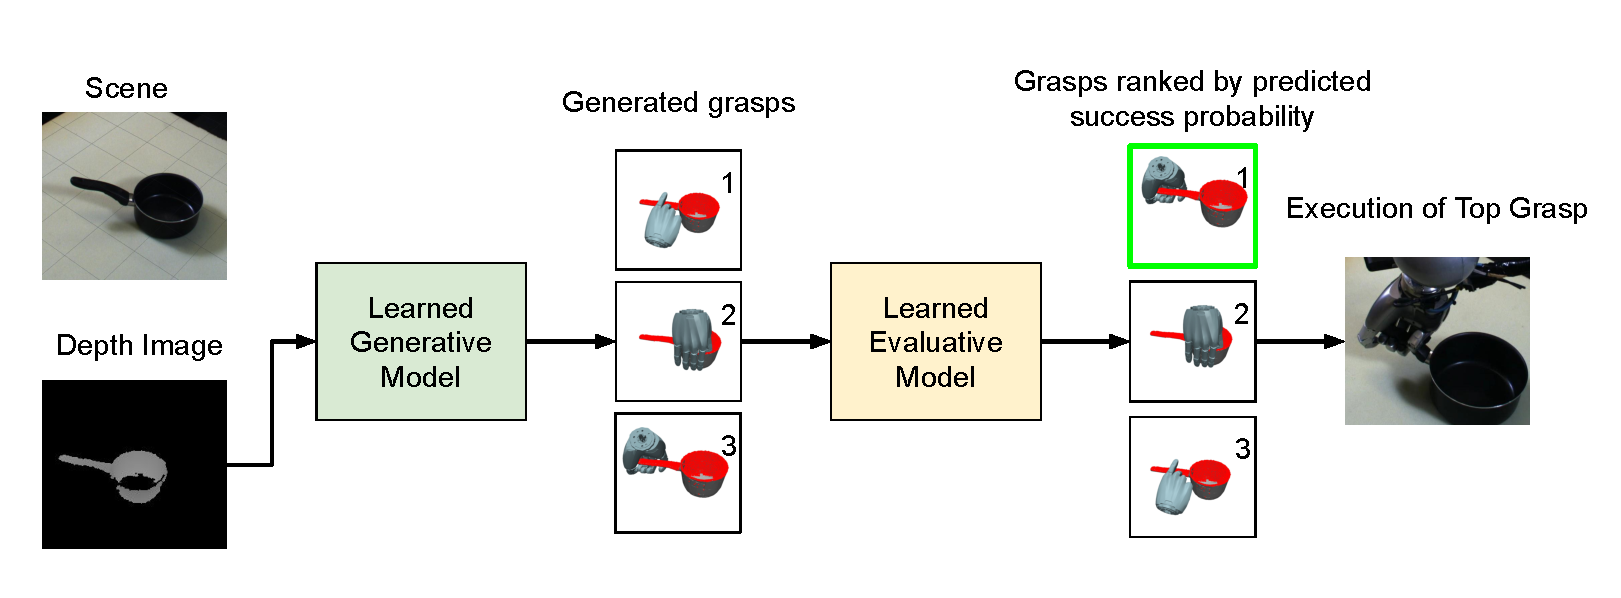
\includegraphics[width=\columnwidth]{images/GEAarchitecture.pdf}
  \end{center}
  \caption{Our grasping architecture. When shown an object, a generative model (GM) produces grasps, ranked according to its likelihood model. These are re-ranked by the predicted success probability of the evaluative Model (EM).The top ranked grasp is executed \label{fig:systemArchitecture}}
\end{figure}

The contributions of this paper are as follows. First, we present a data set of 2.4m simulated dexterous grasps, available to evaluate dexterous grasping algorithms. Second, we release the source code of the dexterous grasp simulator, which can be used to visualise the data set and gather new data.\footnote{The code and simulated grasp data set are available at \href{https://rusen.github.io/DDG}{https://rusen.github.io/DDG}.} Third, we combine an existing learned generative model with multiple learned evaluative models that are trained from simulated grasps proposed by the generative model. Fourth, we present an extensive evaluation of all these models on our simulated data set. Fifth, we compare the two most promising variants on a real robot with a data set of objects in challenging poses. Finally, we perform a deep dive into the simulation results.

The model variants are organised in three dimensions. First, we employ two different generative models (GM1 \cite{kopicki2015ijrr} and GM2 \cite{kopicki2019ijrr}), one of which (GM2) is designed specifically for single view grasping. Second, we use two different back-bones for the evaluative model, VGG-16 and ResNet-50. Third, we experiment with two optimisation techniques--gradient ascent (GA) and stochastic annealing (SA)--to search for better grasps using the evaluative model as an objective function.

%The first contribution of this paper is the first generative-evaluative architecture where both generative and evaluative models are learned. Second, three novel evaluative networks, based on existing VGG-16 and ResNet-50 architectures, were proposed. Finally, a grasp simulation dataset containing 2M+ grasps on 295 objects, along with the simulator code will be released to to the community. In order to simulate the wide range of physical variations that real world objects have, a data set is acquired by simulation of  grasps proposed by the generative models on novel objects. We vary the physical characteristics of the objects in each simulated scene (mass, friction) which the robot can not observe. This dataset was used to train three evaluative neural networks. The evaluative models were then used to rank grasps produced by the generative models (GM1 and GM2) in real robot experiments. 

%The paper builds upon two existing generative grasp models that are learned from a small number of demonstrated grasps using the data-efficient method for LfD. Unlike other approaches to deep grasping, which are restricted to power-grasps, the methods are able to perform a wide variety of grasps, including pinch, rim, power, and handle grasps, and to use additional fingers to provide bracing.

The paper is structured as follows. First, we discuss related work. Second, we describe the design of the grasp simulation, the generation of the data set. Third, the proposed generative evaluative architecture is described and the different architectures employed for the evaluative model are explained, including the optimisation variants of the evaluative model. Fourth, a simulation-based experimental study of the proposed methods is presented. Fifth, we present the real robot study. Finally, we extend the simulation analysis further by examining the inner workings of the best performing model. 


\section{Background and Related Work}

% * <jeremy.l.wyatt@gmail.com> 2018-01-29T09:06:15.090Z:
% 
% %Give a good overview of the shape of both dexterous grasping, grasping novel objects, and deep networks for grasping.
% 
% Levine-both simulation and 800k grasping papers will be mentioned here. Our method does not perform any grasp planning. Our contribution is a grasp evaluation method that aims to understand the relationship between the point cloud and grasp parameters from the point of view of the camera. 
% 
% 
% ^.

Learning for robot grasping has made steady progress. There are probabilistic machine learning techniques employed for surface estimation for grasping \cite{dragiev2011gaussian}; data efficient methods for learning dexterous grasps from demonstration \cite{ben-amor2012a,kopicki2015ijrr,detry2012a}; logistic regression for classifying grasp features from images \cite{saxena2008a}; and for autonomous learning \cite{detry2010a}. Deep learning is a recent approach to grasping. Most work is for two finger grippers. Approaches either learn an evaluation function for an image-grasp pair \cite{levine16,lenz2015deep,gualtieri2016high,mahler2017dex,pinto2016supersizing,johns2016deep}, learn to predict the grasp parameters \cite{redmon2015real,kumra2017iros} or jointly estimate both \cite{morrison18}. The quantity of real training grasps can be reduced by mixing real and simulated data \cite{bousmalis2017using}. 

A small number of papers have explored deep learning as a method for dexterous grasping. \cite{lu2017planning,varley2015generating,veres2017modeling,zhou20176dof,kappler2015leveraging}. All of these use simulation to generate the training set for learning. Kappler \cite{kappler2015leveraging} showed the ability of a CNN to predict grasp quality for multi-fingered grasps, but uses complete point clouds as object models and only varies the wrist pose for the pre-grasp position, leaving the finger configurations the same. Varley \cite{varley2015generating} and later Zhou \cite{zhou20176dof} went beyond this, each being able to vary the hand pre-shape, and predicting from a single image of the scene. Each of these posed search for the grasp as a pure optimisation problem (using simulated annealing or quasi-Newton methods) on the output of the CNN. They all, also, take the approach of learning an evaluative model, and generate candidates for evaluation uninfluenced by prior knowledge. Veres \cite{veres2017modeling}, in contrast, learns a deep generative model. Finally Lu \cite{lu2017planning} learns an evaluative model, and then, given an input image, optimises the inputs that describe the wrist pose and hand pre-shape to this model via gradient descent, but does not learn a generative model. In addition, the grasps start with a heuristic grasp which is varied within a limited envelope. Of the papers on dexterous grasp learning with deep networks only two approaches \cite{varley2015generating,lu2017planning} have been tested on real grasps, with eight and five test objects each, producing success rates of 75\% and 84\% respectively. An important restriction of both of these methods is that they only plan the pre-grasp, not the finger-surface contacts and are thus limited to power-grasps.

Thus, in each case, either an evaluative model is learned but there is no learned prior over the grasp configuration able to employed as a generative model; or a generative grasp model is learned, but there is no evaluative model learned to select the grasp. Our novelty is thus to bring together a data-efficient method of learning a good generative model with an evaluative model. As with others, we learn the evaluative model from simulation, but the generative model is learned from a small number of demonstrated grasps. 


%n learning to grasp divides into two categories, that we label {\em generative} and {\em evaluative} respectively. We quickly summarise the relationship between this paper and these two.
%
%Generative approaches to grasping include the work of detry et al, kopicki et al, these methods learn distributions of grasps from positive examples. In the case of detry, saxena, these are pinch grasps that are associated with features extracted from monocular or stereo images. Both those pieces of work were restricted to pinch grasps. Both Saxena and Detry require significant training samples, but Detry used real grasps, whereas Saxena used simulation to generate training exemplars. Other approaches use LfD rather than autonomous exploration, as this can significantly reduce the training data required. Peters et al introduced a method for generative grasping by grasp warping, demonstrating an ability to handle new objects of a similar global shape to the training objects. Kopicki et al introduced a factored generative model, showing grasp transfer to novel objects from one example of each grasp type. This is the method than we replicate and build on in our work.
%
%Evaluative approaches to grasping include the work of levine, in which a farm of fourteen robot were used over a two month data gathering period. This data is used to train a neural network that predicts the probability of success of a pinch grasp conditional on an image. In that work the only input is an RGB image, but other approaches to deep grasping tenpas use depth images. However, all these approaches are all data intensive. 
%
%The work that is closest to ours, and the only paper of which we are aware on deep learning applied to dexterous grasping, is that of Hermans et al. 

\section{Data Efficient Learning of a Generative Grasp Model from Demonstration}

%Describe, in new words, the method from IJRR.
This section describes the generative model learning. We employ the method of \citet{kopicki2015ijrr}, which learns a generative model of a dexterous grasp from a demonstration (LfD). That paper posed it as the problem of learning a factored probabilistic model. The method is split into a model learning phase, a model transfer phase, and the grasp generation phase. 

\subsection{Model learning}
The model learning is split into three parts: acquiring an {\em object model}; using this object model, with a demonstrated grasp, to build a {\em contact model} for each finger link in contact with the object; and acquiring a {\em hand configuration model} from the demonstrated grasp. After learning the object model can be discarded.

\subsubsection{Object model}
First, a point cloud of the object used for the demonstrated grasp is acquired by a depth camera, from several views. Each point is augmented with the estimated principal curvatures at that point and a surface normal. Thus, the $j^{th}$ point  in the cloud gives rise to a feature $x_j=(p_j, q_j, r_j)$, with the components being its position $p_j \in \mathbb R^3$, orientation $q_j \in SO(3)$ and principal curvatures $r_j=(r_{j,1},r_{j,2}) \in \mathbb R^2$. The orientation $q_j$ is defined by $k_{j,1},k_{j,2}$, which are the directions of the principal curvatures.  For later convenience we use $v=(p,q)$ to denote position and orientation combined. These features $x_j$ allow the object model to be defined as a kernel density estimate of the joint density over $v$ and $r$.
\begin{equation}
\om(v, r) \equiv \pdf^\om(v, r) \simeq \sum_{j=1}^{K_O} w_j \mathcal{K}(v, r|{x_j}, \sigma_{x})
%RD: mu and sigma are not properly defined.
\label{eq:om}
\end{equation}
where $\om$ is short for $\pdf^\om$, bandwidth $\sigma_{x} = (\sigma_{p}, \sigma _{q}, \sigma_{r})$, $K_O$ is the number of features $x_j$ in the object model, all weights are equal $w_j = 1/{K_O}$, and $\mathcal{K}$ is defined as a product:
\begin{equation}\label{eq:kernel_in_se3}
\mathcal{K}(x | \mu, \sigma) = \mathcal{N}_3(p| \mu_p, \sigma_p) \Theta(q| \mu_q, \sigma_q) \mathcal{N}_2(r| \mu_r, \sigma_r)
\end{equation}
where $\mu$ is the kernel mean point, $\sigma$ is the kernel bandwidth, $\mathcal{N}_n$ is an $n$-variate isotropic Gaussian kernel, and ${\Theta}$ corresponds to a pair of antipodal von Mises-Fisher distributions.
\begin{figure*}[t]
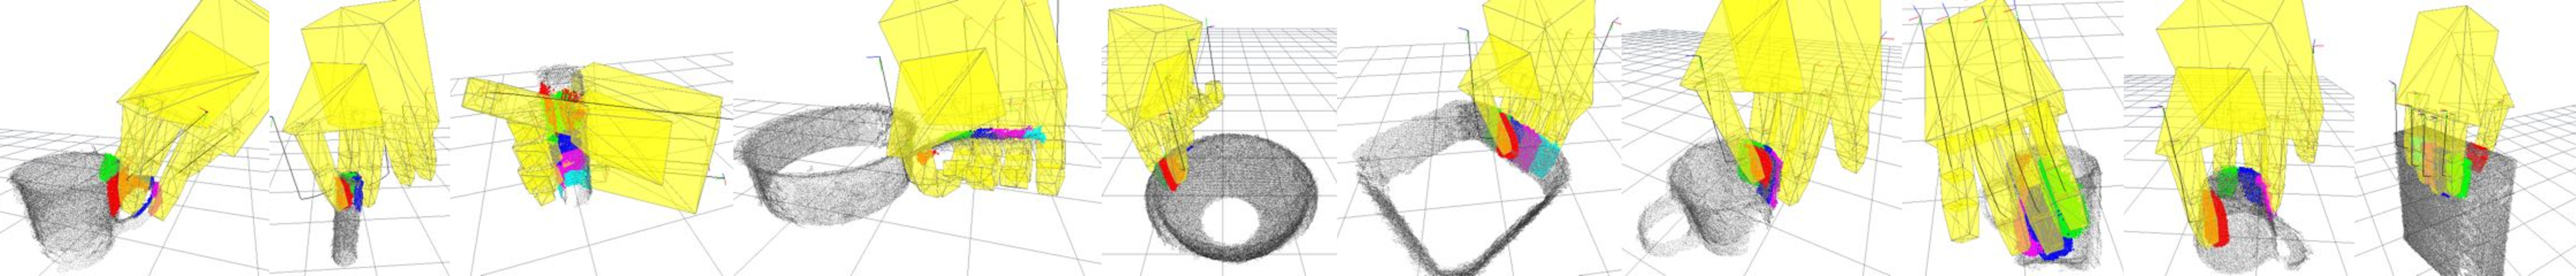
\includegraphics[width=\textwidth]{images/training-examples}
%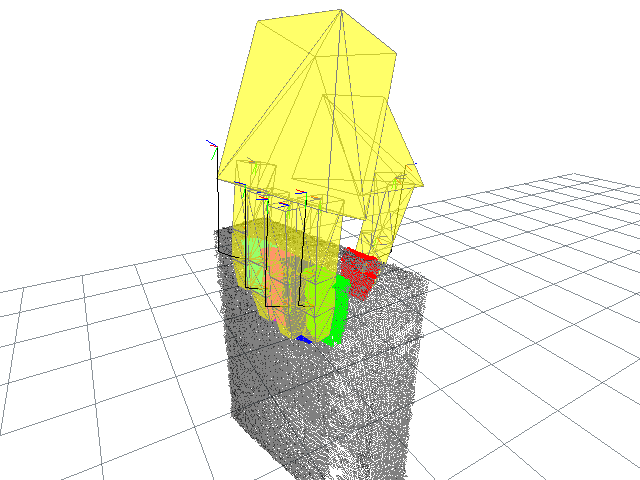
\includegraphics[width=0.1\textwidth]{images/contact-viewall2}
%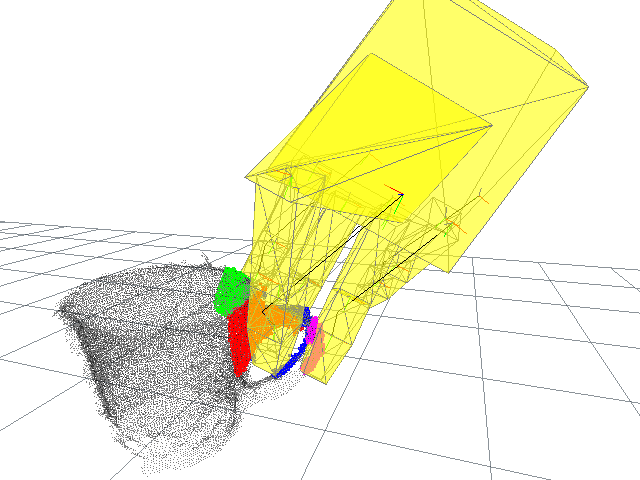
\includegraphics[width=0.1\textwidth]{images/contact-viewall3}
%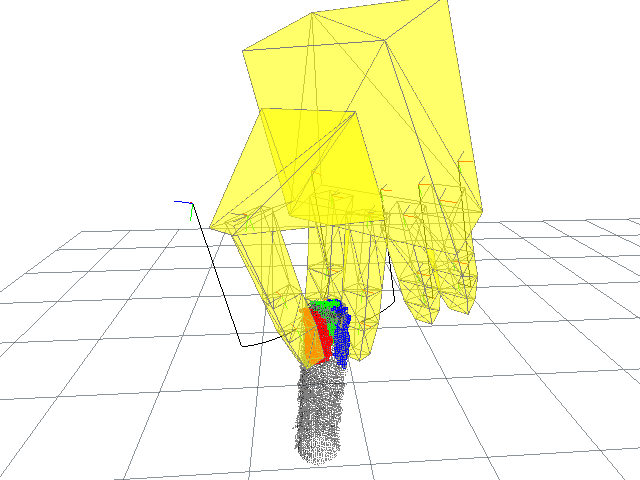
\includegraphics[width=0.1\textwidth]{images/contact-viewall4}
%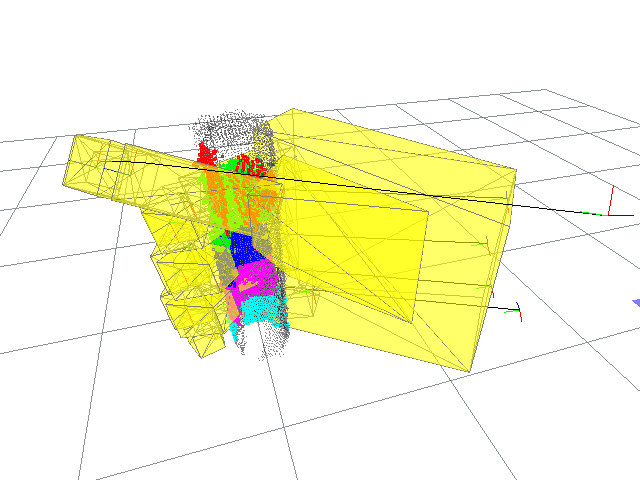
\includegraphics[width=0.1\textwidth]{images/contact-viewall5}
%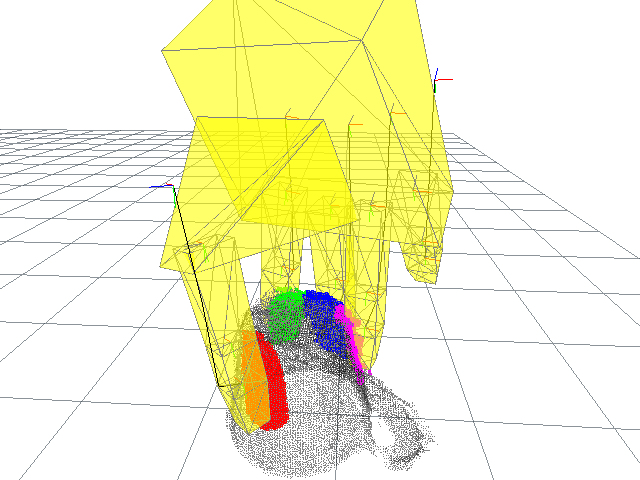
\includegraphics[width=0.1\textwidth]{images/contact-viewall6}
%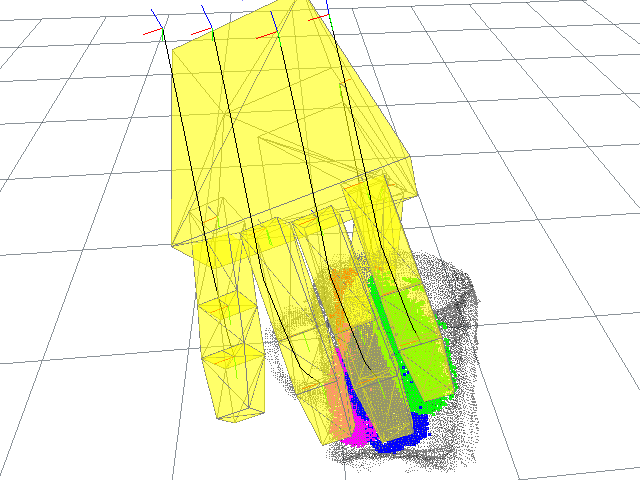
\includegraphics[width=0.1\textwidth]{images/contact-viewall7}
%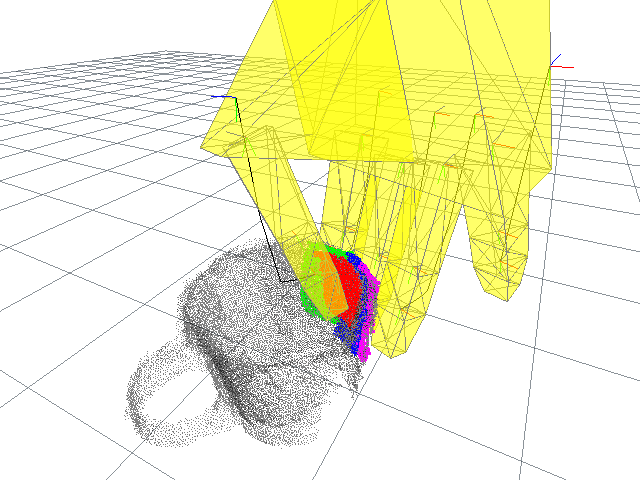
\includegraphics[width=0.1\textwidth]{images/contact-viewall8}
%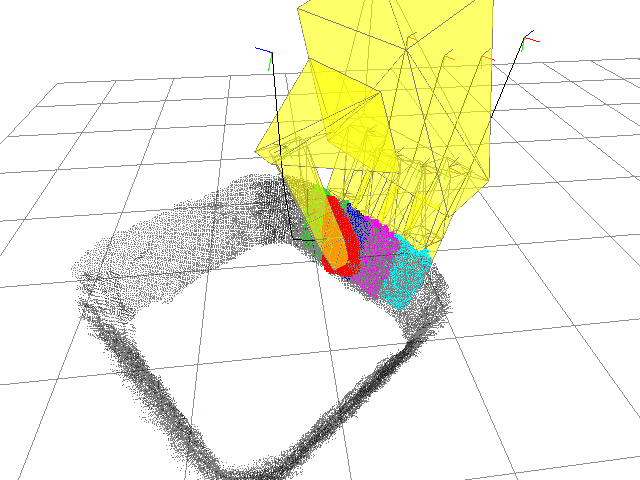
\includegraphics[width=0.1\textwidth]{images/contact-viewall9}
%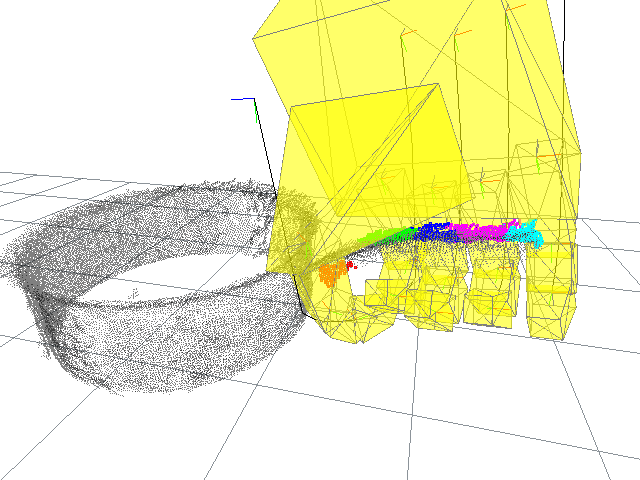
\includegraphics[width=0.1\textwidth]{images/contact-viewall10}
\caption{The ten training grasps for the generative model. The final hand pose is shown in yellow, the sensed point cloud in black, and the parts of the point cloud that contribute to each contact model are coloured by the associated link. \label{fig:generative-training}}
\end{figure*}
\subsubsection{Contact models}
When a grasp is demonstrated the final hand pose is recorded. This is used to find all the finger links $L$ and surface features $x_j$ that are in close proximity. A contact model $M_i$ is built for each finger link $i$. Each feature in the object model that is within some distance $\delta_i$ of finger link $L_i$ contributes to the contact model $\cm_i$ for that link. This contact model is defined for finger link $i$ as follows:
\begin{equation}
\cm_i(u, r) \equiv \pdf^\cm_i(u, r) \simeq \frac{1}{Z} \sum_{j=1}^{K_{M_i}} w_{ij} \mathcal{K}(u, r | {x_j}, \sigma_{x})
%RD: mu and sigma are not properly defined.
\label{eq:cm}
\end{equation}
where $u$ is the pose of $\rl_i$ relative to the pose $v_j$ of the $j^{\mathnormal{th}}$ surface feature, $K_{M_i}$ is the number of surface features in the neighbourhood of link $L_i$, $Z$ is the normalising constant, and $w_{ij}$ is a weight that falls off exponentially as the distance between the feature $x_j$ and the closest point $a_{ij}$ on finger link $L_i$ increases:
\begin{equation}
w_{ij} = \begin{cases}\exp(-\lambda ||p_j-a_{ij}||^2) \quad &\textnormal{ if } ||p_j-a_{ij}|| < \delta_i\\
0 \quad &\textnormal{ otherwise},\end{cases}
\label{eq:learning.modeldist.wgh}
\end{equation}
The key property of a contact model is that it is conditioned on local surface features likely to be found on other objects, so that the grasp can be transferred. We use the principal curvatures $r$, but many local surface descriptors would do. %A contact model can be visualised by marginalising out the dimensions for the rigid body transformation $u$, showing us the distribution over the local curvatures that finger link $L_i$ experienced in the demonstrated grasp. 
%
%\begin{figure*}
%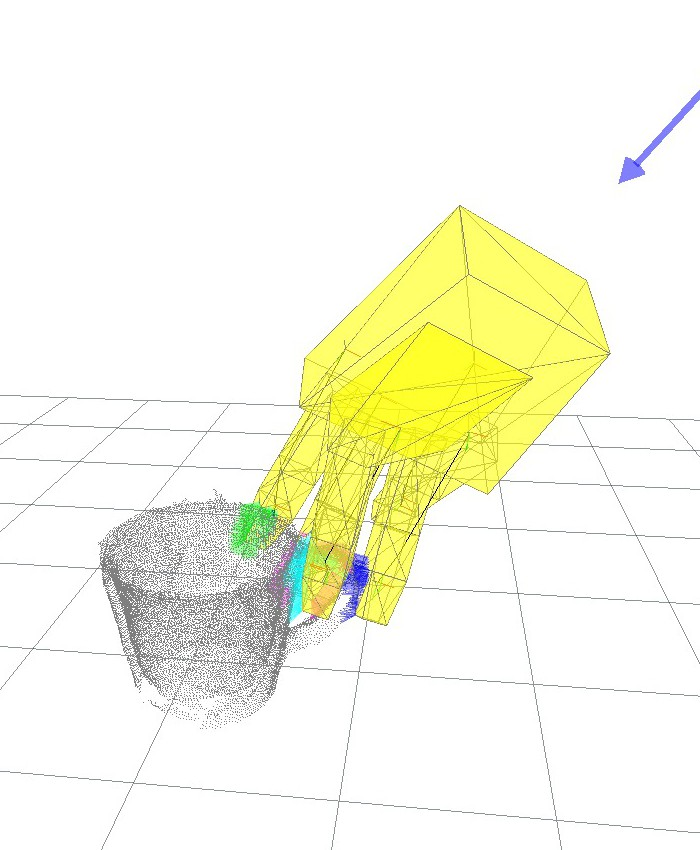
\includegraphics[height=2cm]{images/contact-model-learning/handle-grasp}
%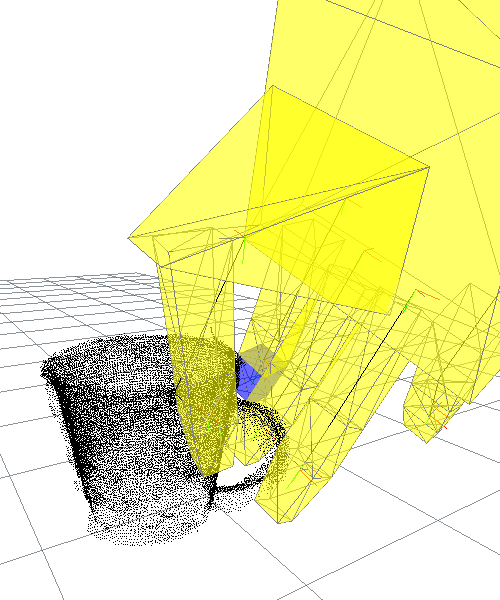
\includegraphics[height=2cm]{images/contact-model-learning/link8}
%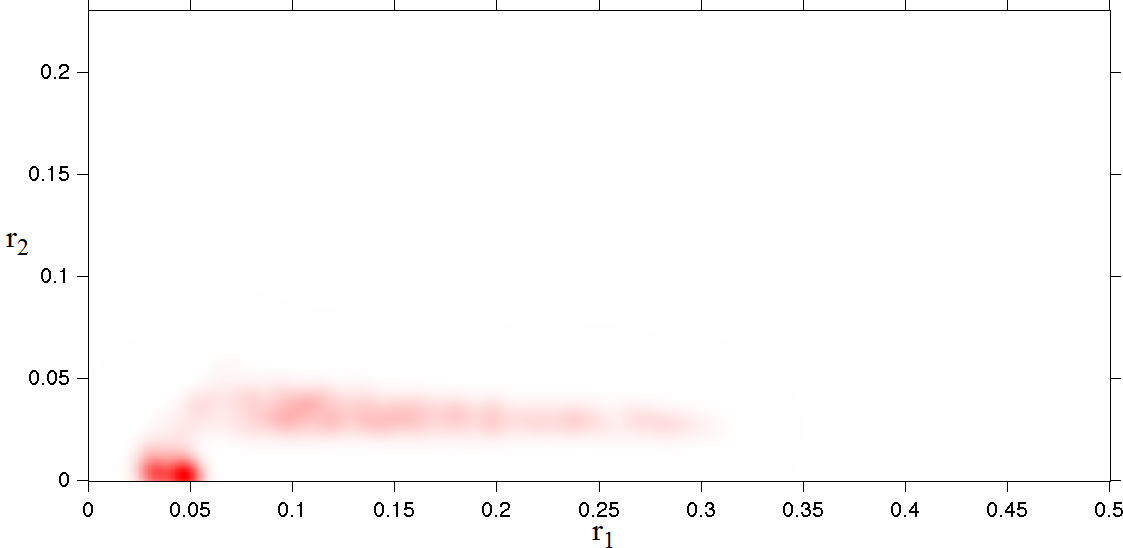
\includegraphics[height=2cm]{images/contact-model-learning/handle_model_08_00778r}
%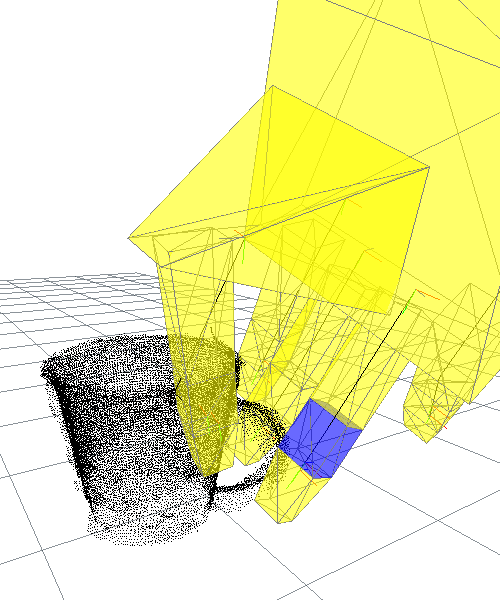
\includegraphics[height=2cm]{images/contact-model-learning/link15}
%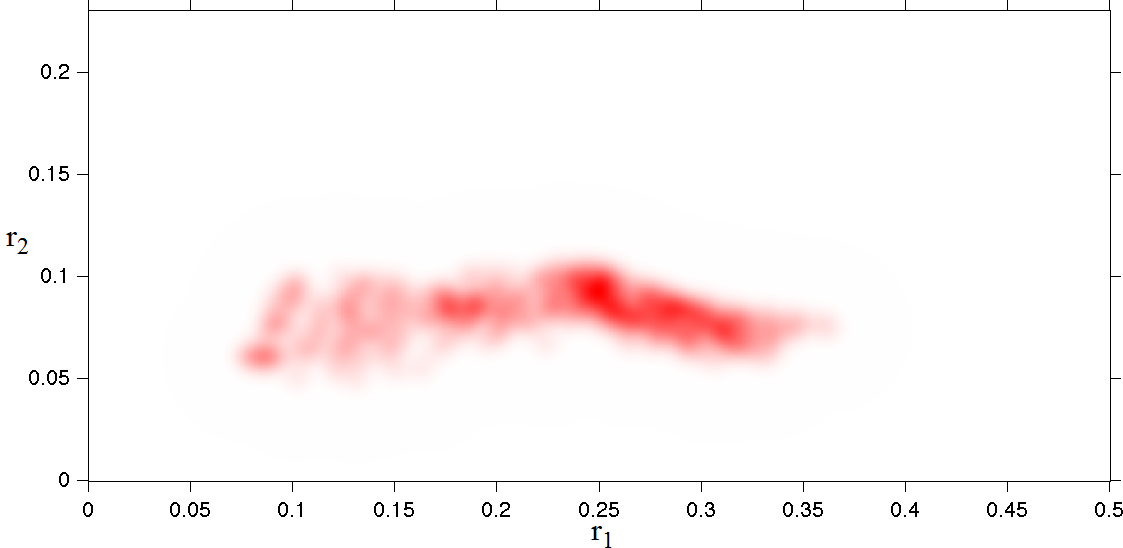
\includegraphics[height=2cm]{images/contact-model-learning/handle_model_15_00329r}
%  \caption{A training grasp and some contact models arising from it.}
%  \label{fig:contactModels}
%\end{figure*}

\subsection{Hand configuration model}
In addition to a contact model for each finger-link, a model of the hand configuration $h_c \in \mathbb R^D$ is recorded, where $D$ is the number of DoF in the hand. $h_c$  is recorded for several points on the demonstrated grasp trajectory as the hand closed. The learned model is:
\begin{equation}
\hc(h_c) \equiv \sum_{\gamma \in [-\beta, \beta]} w({h_c(\gamma)}) \mathcal{N}_D(h_c|h_c(\gamma), \sigma_{h_c}) 
\label{eq:hc}
\end{equation}
where $w({h_c(\gamma)}) = \exp(-\alpha \|h_c(\gamma) - h^g_c \|^2)$; $\gamma$ is a parameter that interpolates between the beginning ($h^t_c$) and end ($h^g_c$) points on the trajectory, governed via \eq\ref{eq:learning.configmodel.config} below; and $\beta$ is a parameter that allows extrapolation of the hand configuration.
\begin{equation}
h_c(\gamma) = (1 - \gamma)h^g_c + \gamma h^t_c
\label{eq:learning.configmodel.config}
\end{equation}
\subsection{Grasp Transfer}
When presented with a new object $o_{new}$ the contact models must be transferred to that object. A partial point cloud of $o_{new}$ is acquired (from a single view) and recast as a density, $\om_{new}$, again using \eq \ref{eq:om}. The transfer of each contact model $\cm_i$ is achieved by convolving $\cm_i$ with $\om_{new}$. This convolution is approximated with a Monte-Carlo method, resulting in an kernel density model of the pose $s$ of the finger link $i$ (in workspace coordinates) for the new object. The Monte-Carlo procedure samples poses for link $L_i$ on the new object. The $j^{th}$ sample is $\hat{s}_{ij}=(\hat{p}_{ij},\hat{q}_{ij})$. Each sample $\hat{s}_{ij}$ is weighted $w_{ij}$ by its likelihood. These samples are used to build what we term the query density:
\begin{equation}
\qd_i(s) \simeq \sum^{K_{Q_i}}_{j=1} w_{ij} \mathcal{N}_3(p|{\hat{p}_{ij}}, \sigma_{p}) \Theta(q|{\hat{q}_{ij}}, \sigma_{q})%, \quad i = 1, ..., N_L
\label{eq:qd.approx}
\end{equation}
where all the weights are normalised, $\sum_j w_{ij} = 1$. A query density is constructed for every contact model and the new object. These query densities, together with the hand configuration model, are then used to generate grasps. Query density computation is fast, taking $<0.5$ second per grasp model.
\begin{figure*}[t]
\begin{center}
  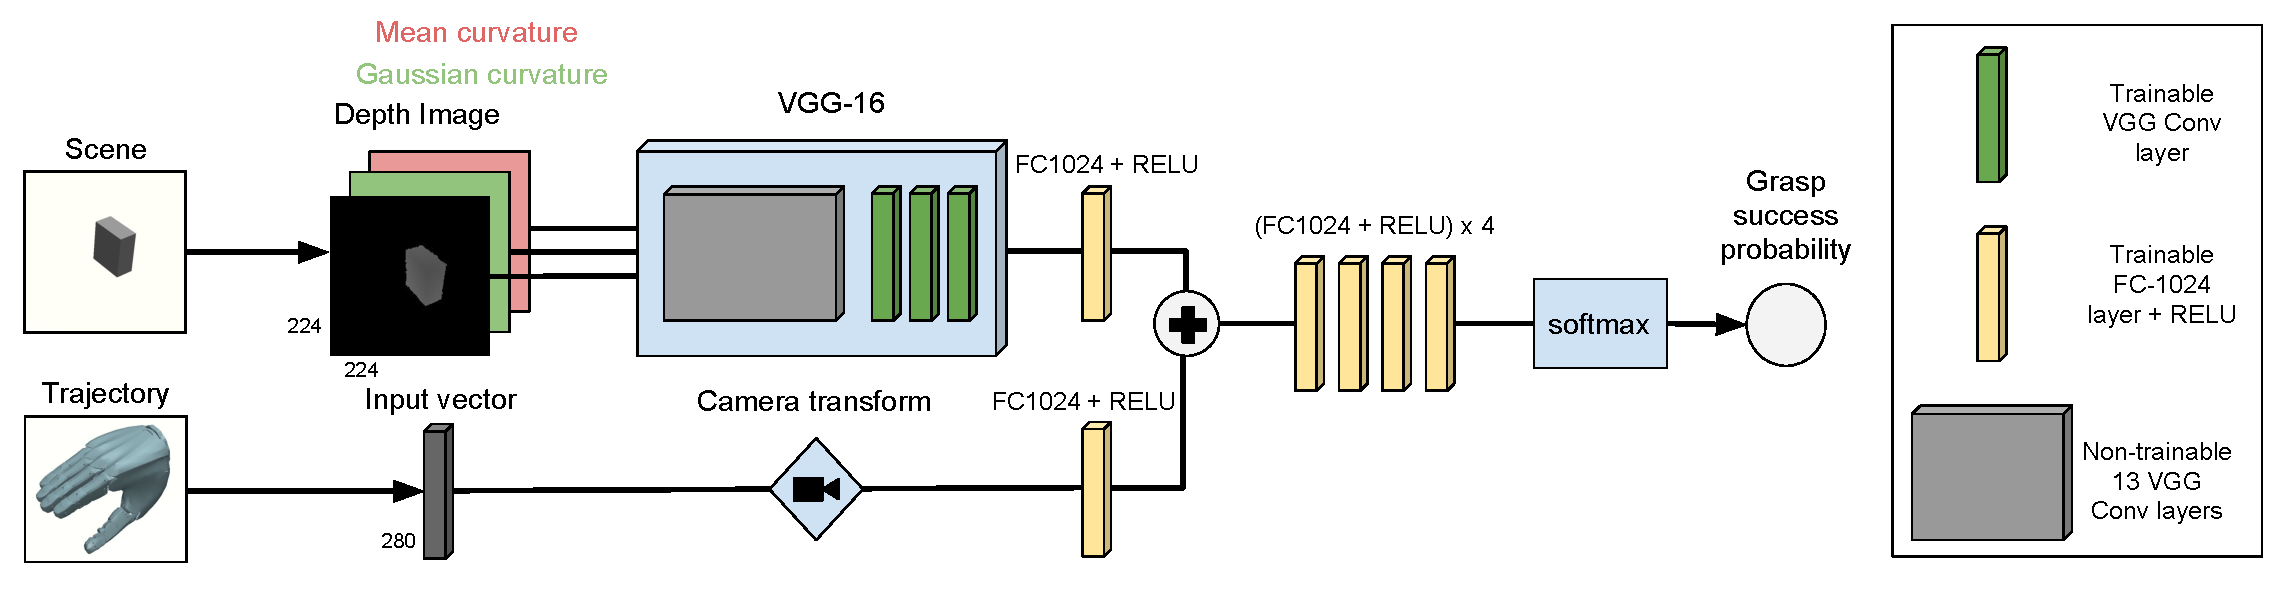
\includegraphics[width=0.9\textwidth]{images/networkArchitecture.pdf}
  \end{center}
  \caption{The evaluative network architecture.}
\label{fig:networkArchitecture}
\end{figure*}
\subsection{Grasp generation}
Candidate grasps may be generated as follows. Select a query density $k$ and take a sample  $s_k \sim \qd_{k}$. Then, take a sample $h_c \sim C$ from the hand configuration model. This pair of samples together define, via the hand kinematics, a complete grasp $h=(h_w,h_c)$, where $h_w$ is the pose of the wrist and $h_c$ is the configuration of the hand. The initial grasp is then improved by stochastic hill-climbing on a product of experts:
\begin{equation}
\argmax{(h_w, h_c)} \hc(h_c) \prod_{\qd_i \in \mathcal{Q}} \qd_i\left(k_{i}^{\mathrm{for}}\left(h_w, h_c\right)\right)
\label{eq:grasping.product}
\end{equation}
This generate and improvement process has periodic pruning steps, in which only the higher likelihood grasps are retained. It can be run many times, thus enabling the generation of many candidate grasps. In addition, a separate generative model can be learned for each demonstrated grasp. Thus, when presented with a new object, each grasp model can be used to generate and improve grasps. We generate and optimise 100 grasps per grasp type. Finally, the many candidate grasps generated from each grasp model can be compared and ranked according to their likelihoods. The product of experts formulation, however, only ensures that the generated grasps have high likelihood according to the model. There is no estimate of the probability that the grasp will succeed. This motivates the dual architecture in this paper. We now turn to the learning method we used to re-rank the grasps according to predicted success probability. 

\subsection{Training Grasps for Our Study}

For the purposes of our study, ten example grasps were provided. These are visualised in Figure~\ref{fig:generative-training}. In contrast to \cite{kopicki2015ijrr}, although seven views of each training object were taken, we trained a separate generative model for each view. This led to a total of 70 generative models being learned, one for each grasp-view combination. In addition, we made two innovations to the generative model. In the first, because of the view based training, we filter surface normals on the object model so that for each contact model we only consider points on the object surface with surface normals within +/- 90 degrees of the surface of the finger link. In the second, rather than globally selected the best grasps during optimisation---regardless of the training grasp type, as in the algorithm reported in \cite{kopicki2015ijrr}---we select half globally across all training grasp types, and half we force to be evenly spread across the grasp types. This enables us to keep a broad range of grasp options open to us for evaluation, and thus improves performance.
 \label{section:generative}

\section{The Evaluative Model} \label{section:learning}

The generative model generates 1000 grasps for a new object within 15 seconds on a 2x Intel Xeon E5-2650 v2 Eight Core 2.6GHz. There is, however, no estimate of the probability of grasp success. This the purpose of the evaluative model. Deep networks have been shown to learn good evaluative models of grasp success for two finger grippers and for dexterous hands (Barrett, Allegro) performing power grasps.  
%In this section, our evaluative deep network architecture is described. In the following section, the simulation used to generate the training data is detailed.
%First, the generative model largely ignores global information about the object; relying instead on global information about the hand shape, and local information about finger-object contacts. To predict grasp success probability we need a learner that somehow takes into account global information, such as global shape, mass, mass distribution, friction coefficients, deformability, etcetera. The difficulty with this is that, given a single depth image, the learner does not have direct access to these. Thus, they cannot be estimated, but all that can be learned is the association Second, the 

%It is time-consuming and expensive to collect real grasp data with using robotic arms with dexterous hands. Unlike gripper + arm combinations which require relatively less supervision \cite{Levine1}, dexterous hands can be much more fragile due to their complexity. Advances in physics simulators have made it possible to re-create robotic experiment setups in simulation. We created a simulated experimental setup in order evaluate grasp, which allowed us to collect as much data as needed in a short period of time with no supervision.
We now present the architecture (Figure~\ref{fig:networkArchitecture}) of our evaluative network $f(I_t, h_t)$, where $I^t$ is a colourized depth image of the object, and $h_t = (h_{tw}, h_{tc})$ gives the sequence of wrist poses and hand configurations for a grasp, expressed in the camera frame. The network outputs a grasp success probability for image-grasp pair $I_t$, $h_t$. Section~\ref{section:simulation} gives details of the simulation used to generate the training data.

% The purpose of the network is to learn the relationship between the point cloud, given as a colorized depth image, and grasp (hand shape) parameters which encode the configuration of the hand with respect to the camera frame. This is a complex task, as the kinematic model of the hand is unknown to the network, and it has to consider each grasp as a black box: The network knows the inputs that configure the hand, including the joint positions, and only has access to the outcome in the form of success/failure. 
% Talk more about the architecture
For visual processing, we use the VGG-16 network pre-trained on ImageNet. The final three layers are fine-tuned, while the first 13 layers are frozen. Pre-processing segments the table plane from the object point cloud of the object. The segmented $640 \times 480$ depth image $I_{t}^{depth}$ is cropped to a window of $460 \times 460$, located in the image centre. Then, it is down-sampled to $224 \times 224$. The colourization creates a $224 \times 224$ 3-channel image $I_t$. The channels  are the mean curvature, the Gaussian curvature, and the depth. %The formula of mean curvature is $h = {gr}_{xx} + {gr}_{yy}$, where ${gr}_{xx}$ is the second gradient in horizontal direction in a $1 \times 3$ window, and ${gr}_{yy}$ is its vertical counterpart. Similarly, Gaussian curvature $k = {gr}_{xx} \times {gr}_{yy} - ({gr}_{xy})^2$.
The hand trajectory $h_t$ comprises 10 way-points, each of 28 dimensions (20 for the finger joint angles, 1 for the grasp type, and 7 for the wrist pose), giving 280 dimensions. This is transformed to 1024 using a single layer. This and the output of the final VGG layer are added together unit-wise. Then there are four fully connected layers each comprising 1024 RELU nodes. The output is a grasp success/failure probability, encoded by two softmax nodes.  We train using the cross-entropy loss function:
\begin{equation}
H_{y'}(y) := - \sum_{i} ({y_i' \log(y_i) + (1-y_i') \log (1-y_i)})
\label{equation:crossentropy}
\end{equation}
where $y_i'$ is the ground truth success (1) or failure (0); $y_i = f(I_i, h_i)$ is the predicted grasp success of grasp trajectory $h_i$, and $I_i$ is the associated colourized depth image of grasp $h_i$.
\begin{figure}
\begin{center}
  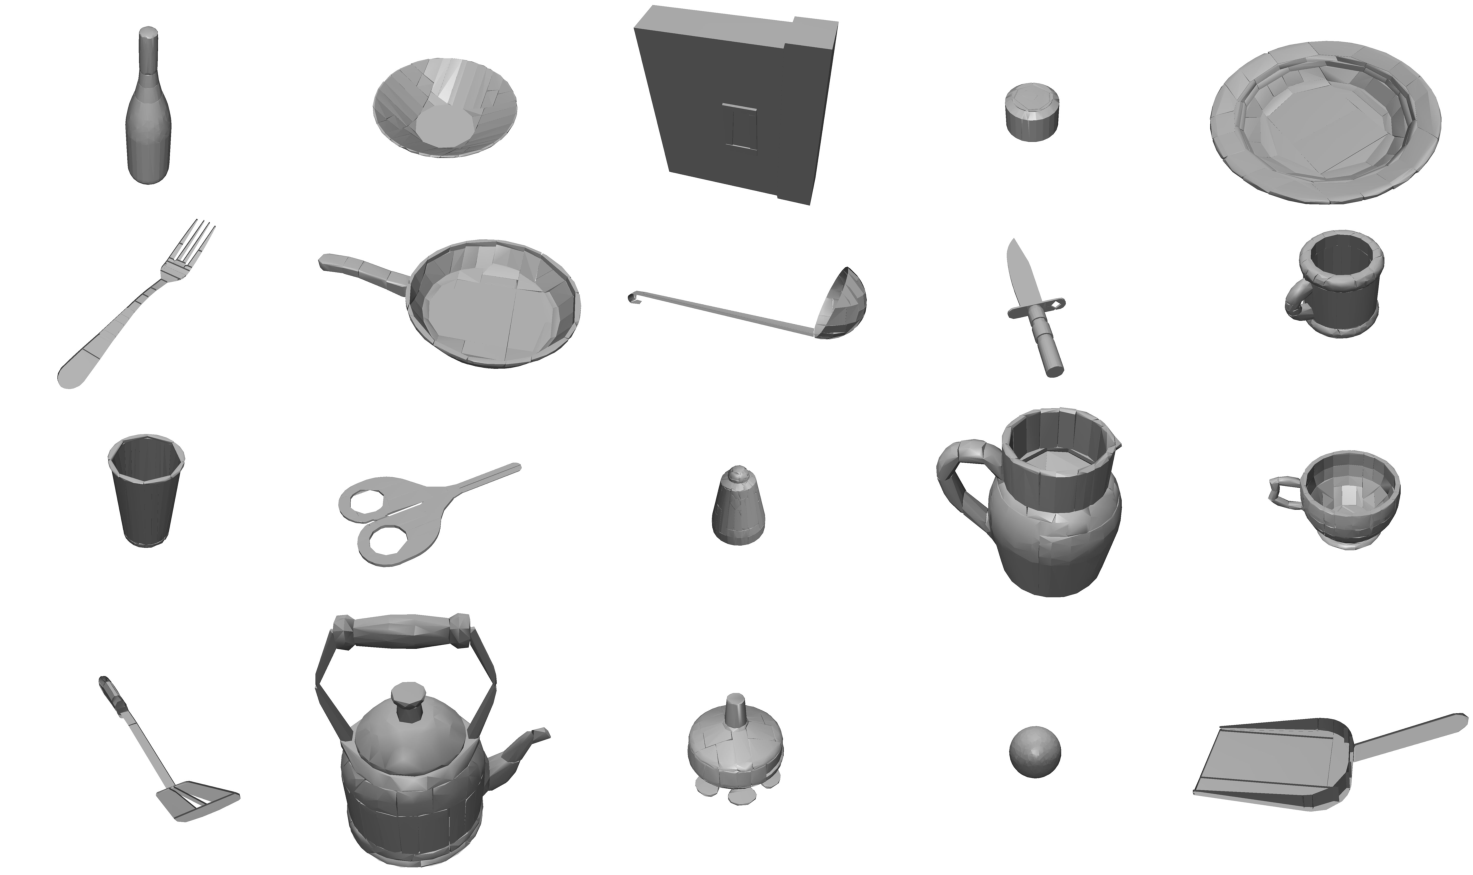
\includegraphics[width=0.9\linewidth]{images/allObjects-small.pdf}
  \end{center}
  \caption{Sample objects from all classes in the 3D model dataset.}
  \label{fig:allObjects}
\end{figure}
We trained our network on a data set of 441,312 grasps. We now describe the simulation used to generate a realistic training set. % o 7000 distinct scenes, where each scene contains a random instantiation of one of the objects in the dataset with varying rigid body transformations applied, as well as friction and weight changes. The network was tested on 80000 grasps on 1200 scenes of unseen objects, as well as real robot experiments, as explained in Section \ref{section:experiments}. In order to make a direct comparison with Kopicki et al. \cite{kopicki2015ijrr}, we pick top grasps based on both the original ranking, as explained in Section \ref{section:generative}, and according to the predicted success probabilities by the network. 

%We opted to use a grasp success prediction network due to the fact that the grasp generator function, explained in the previous chapter, provides alternatives of most intuitive types of grasps. A logical extension of this work would be to pair our learning algorithm with a grasp generator network, which we consider as future work.

%Overall network architecture. VGG summary. Description of new layers. Representation of hand parameters, frames of reference, camera image conversion for VGG, trajectory of wrist and fingers.

\section{Training the Evaluative Model from Simulation} \label{section:simulation}
%Introductory sentences here
In this section, we describe how we generated a realistic simulated data set for dexterous grasping. This captures variations in both observable (e.g. object pose) and unobservable (e.g. surface friction) parameters.

To generate the training set a simulated depth image of a scene containing a single unfamiliar object is generated. Using either of the generative models GM1 or GM2, grasps are generated and executed in simulation. The success or failure of each simulated grasp is recorded. Producing a good simulation for evaluating grasps is non-trivial. An important problem is that the data set must capture the natural uncertainty in unobservable variables, such as mass and friction. Since many of these parameters are unobservable we are thus creating a data set such that the grasp policy must work across a range of variations. This is thus a form of {\em domain randomisation}. A similar technique has been employed by \cite{mahler2017dex}, but we extend it from a single grasp quality metric to full rigid body simulation.

\subsection{Features and Constraints of the Virtual Environment}
\label{subsection:environment}

The collected 3D model dataset contains 294 objects from 20 classes, namely, bottles, bowls, cans, boxes, cups, mugs, pans, salt and pepper shakers, plates, forks, spoons, spatulas, knives, teapots, teacups, tennis balls, dustpans, scissors, funnels and jugs (Figure \ref{fig:allObjects}). All objects in the dataset can be grasped using the DLR-II hand, although there are limitations on how some object classes can be approached. For example, teapots and jugs are not easy to grasp except by their handles due being larger than the hand's maximum aperture, while small objects such as salt and pepper shakers can be approached in more creative ways. The number of objects in each class varies from 1 (dustpan) to 25 (bottles). Long/thin objects such as kitchen utensils are placed vertically in a short, heavy stand in order to make them graspable without touching the table. This reflects the real-world scenario, as attempting to grasp a spatula lying on a table would be dangerous for the robotic hand. In total, 250 objects from all 20 classes were allocated for training and validation, while the remaining 44 objects from 19 classes belong to the test set.

We employ MuJoCo \cite{MuJoCo} as the rigid-body simulator. Due to the fact that collision checking in MuJoCo requires that objects comprise convex parts, all 294 objects were decomposed into convex parts using V-HACD algorithm \cite{V-HACD}. The number of sub-parts varies from 2 to 120.

During the scene creation, the object is placed on the virtual table at a pseudo-random pose. Most objects are placed in a canonical upright pose, and only randomly rotated around the gravity axis (akin to being placed on a turntable). The objects belonging to the mug and cup classes have fully random 3D rotations applied before they are placed on the table, since it is possible to grasp them in almost any setting using the robot hand.

\begin{figure}
  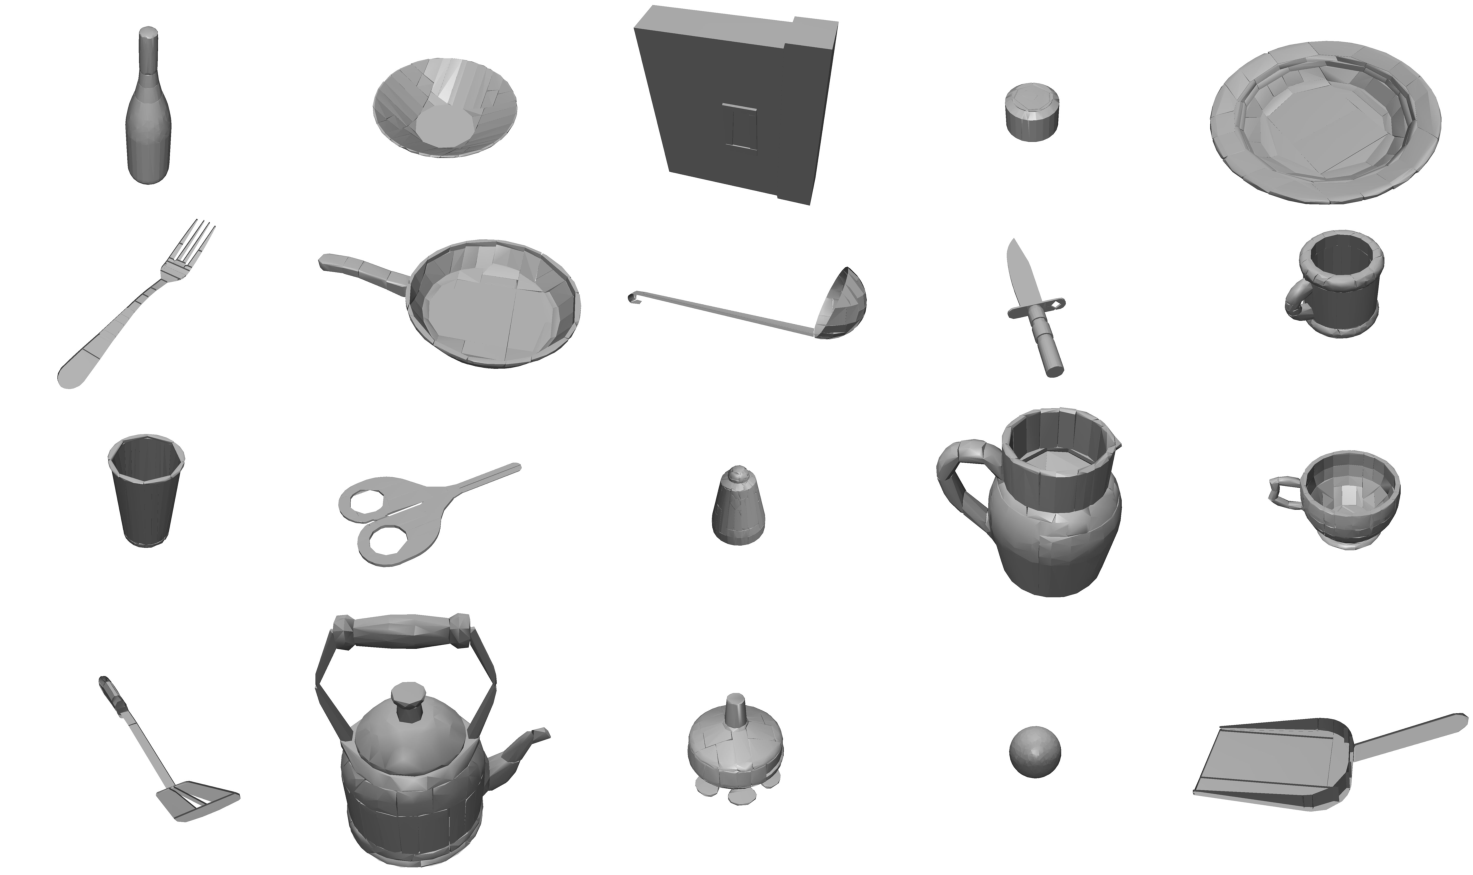
\includegraphics[width=\linewidth]{images/allObjects-small.pdf}
  \caption{A sample of the 294 objects drawn from the 20 object classes.
  \label{fig:allObjects}}
\end{figure}

To achieve domain randomisation, prior distributions for mass, size and frictional coefficient were estimated from real-world data. The properties of simulated objects are sampled from these priors. For each object its mean size, mass and friction coefficient are matched to a real counterpart. For each trial, the size is randomly scaled by a factor in the range [0.9,1.1], while remaining within the grasp aperture of the hand. Object mass is uniformly sampled from a category specific range, estimated from real objects (Table~\ref{fig:weights}). The friction coefficient of each object is sampled from a range of $[0.5, 1]$ in MuJoCo default units, intended to simulate surfaces from low-friction (metal) to high-friction (rubber). This variation is critical to ensuring that the evaluative model will predict the robustness of a grasp to unobservable variations.
\begin{table}[]
\centering
\caption{Mass ranges for each object class (grams).}
\label{fig:weights}
\resizebox{\linewidth}{!}{\begin{tabular}{|l|l|l|l|l|l|l|}
\hline
Bottle & Bowl     & Box     & Can     & Cup    & Fork    & Pan     \\ \hline
30-70  & 50-400   & 50-500  & 200-400 & 30-330 & 40-80   & 150-450 \\ \hline
Plate  & Scissors & Shaker  & Spatula & Spoon  & Teacup  & Teapot  \\ \hline
40-80  & 50-150   & 100-160 & 40-80   & 40-80  & 150-250 & 500-800 \\ \hline
Jug    & Knife    & Mug     & Funnel  & Ball   & Dustpan &         \\ \hline
80-200 & 50-150   & 250-350 & 40-80   & 50-70  & 100-150 &         \\ \hline
\end{tabular}}
\end{table}
 
For depth image simulation the Carmine 1.09 depth sensor installed on the robot is simulated with a modified version of the Blensor Kinect sensor simulator \cite{KinectSimulator}. For each object, we vary the camera orientation and distance from the object, as well as object mass, friction, scale, location and orientation. In order to account for calibration errors in the real world setup, we add a small three-dimensional positional noise to each point in the sensor output.

A 3D mesh-model of the DLR-II hand has been used in the simulator. There are no kinematic constraints on how the hand may grasp an object, other than collisions with the table. To ensure realism, we use impedance control for the hand.
%The reasons for the most critical of these decisions are now given in slightly more detail. First, in order to create a realistic simulation environment, we chose the MuJoCo \cite{MuJoCo} physics simulator over other simulators (OpenSim, BulletPhysics, ODE, NVIDIA PhysX) for two reasons: 
%\begin{itemize}
%\item MuJoCo uses generalized coordinates and optimization-based contact dynamics, resulting in fewer numerical instabilities,
%\item MuJoCo is optimized for the quality of physics as well as its speed, hence improving the quality of the physics simulation.
%\end{itemize}
\begin{figure}
  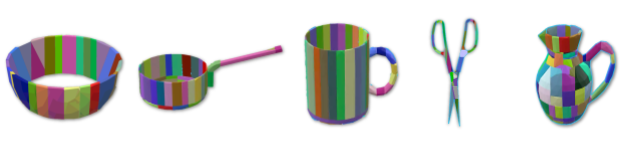
\includegraphics[width=\linewidth]{images/decomposition.png}
  \caption{Approximate convex decomposition of some objects in our dataset. Best viewed in colour.}
  \label{fig:objectDecomposition}
\end{figure}

Some classes are easier to grasp than others. Table \ref{fig:graspperf} shows the success rates of the generated grasps in each class, when attempted with the grasps ranked by the Generative Model (GM1). The sampled grasps perform well on a number of classes including Dustpans, Scissors, Spoons, and Mugs. Some objects can only be grasped in certain ways, i.e. not all 10 training grasps are applicable to all objects.

\begin{table}[]
\centering
\caption{The average and \textbf{top} grasp success rates of GM1 on simulated data.}
\label{fig:graspperf}
\resizebox{\linewidth}{!}{\begin{tabular}{|l|l|l|l|l|l|l|}
\hline
Bottle & Bowl     & Box     & Can     & Cup    & Fork    & Pan     \\ \hline
35.5 - \textbf{47.7}\% & 26.4 - \textbf{61.2}\%   & 16.5 - \textbf{30.1}\%  & 41.4 - \textbf{92.6}\% & 44.7 - \textbf{59.9}\% & 59.6 - \textbf{68.1}\%   & 37.9 - \textbf{57.3}\% \\ \hline
Plate  & Scissors & Shaker  & Spatula & Spoon  & Teacup  & Teapot  \\ \hline
50.2 - \textbf{95.5}\%  & 62.7 - \textbf{69.9}\%   & 47.3 - \textbf{53.3}\% & 57.4 - \textbf{65.7}\%   & 63.4 - \textbf{82.4}\%  & 48.2 - \textbf{91.2}\% & 26.9 - \textbf{23.9}\% \\ \hline
Jug    & Knife    & Mug     & Funnel  & Ball   & Dustpan & \textbf{Total}      \\ \hline
24.9 - \textbf{43.9}\% & 58.3 - \textbf{65.0}\%   & 40.7 - \textbf{80.9}\% & 52.3 - \textbf{65.9}\%   & 28.0 - \textbf{82.8}\%  & 60.1 - \textbf{78.8}\% & 45.8 - \textbf{63.2}\%        \\ \hline
\end{tabular}}
\end{table}

\subsection{Data Collection Methodology}
\label{subsection:dataCollection}

The data set is divided into units called \textit{scenes}, where each scene comprises a single object placed on a table. This object has a specific set of physical parameters, chosen as described below. Many views and grasps are attempted per scene. Below, we specify the time flow of data collection:

\begin{enumerate}
\item A novel instance of an object from the dataset is generated and placed on a virtual table. Variations are applied to object pose, scale, mass, and friction coefficients.
\item A simulated camera takes a depth image $I_s$ of the scene, converted to a point cloud $P_s$. The viewpoint ${elevation}_s$ of the view point is from 30-57 degrees. The ${azimuth}_s$ is sampled from $[0, 2\pi]$. 
\item The positions of all points in the point cloud $P_s$ are shifted by a three-dimensional noise vector sampled from a Gaussian distribution with parameters $\mu=0$ and $\sigma = 0.004$ (unit: meter).
\item Given $P_s$, the chosen generative model (GM1 or GM2) proposes the candidate grasps. For GM1, up to100 grasps are selected. These are the 10 grasps that are highest ranked by the GM for each of the 10 training grasps. For GM2, we select a maximum of 500 grasps: up to 50 grasps from each training grasp.
\item The grasps are applied to the object in simulation.
\item 19 further simulated depth images are taken from other viewpoints around the object, as explained in step 2. Images with fewer than 250 depth points are discarded. We then sample with replacement from the remaining images and associate each sampled image and viewpoint with a grasp created in step 3.
\item The grasp outcome, trajectory and depth image are stored for each trial. The grasp parameters are converted to the camera frame for the associated view.
\end{enumerate}

%Each candidate grasp $h_i = \{w_0, ..., w_{n}\}$ consists of a series of 10 waypoints along : $w_0$, ..., $w_{n}$. A waypoint $w_k$ is a 27-element vector that specifies full configuration of the hand in joint space: 3 dimensions for 3D coordinates and 4 dimensions for the orientation of the wrist, and 20 parameters specifying each finger joint's activation. 
%After a grasp $h_i$ is generated in world coordinates, the waypoints that belong to the grasp are converted to the camera's frame of reference. 
%The goal of our network architecture is to learn which grasps are more likely to succeed given a point cloud, where both input channels are represented in terms of the camera frame of reference. %This point differentiates us from the work of Levine et al. \cite{Levine1}, where camera coordinates are not used. It should be noted that the possible camera locations in our simulated data covers a larger space, with full circular movement $[0, 2\pi]$ on azimuth and $[30-57]$ range in elevation. Our scenes do not have any distinguishing landmarks such as a bin or robot base, which may aid the network in locating the camera in the scene. 

In each scene $S_i$, a number of depth images are taken $\{I_{ik}\}_{k=0}^{20}$, in the manner explained above. The first image $I_{i0}$ is used to generate grasps, as explained in Section \ref{section:generative}. We typically perform 10-500 grasps per scene. Attaching different views to each grasp instead of the seed image $I_{i0}$ ensures there is more variation in terms of viewpoints, resulting in a richer dataset. Typically, performing a grasp takes half the time it takes to acquire an image using the simulated camera.

Once a grasp is performed in simulation, it is considered a success if an object is lifted one metre above the table, and held there for two seconds. If the object slips from the hand during lifting or holding, the grasp is a failure. 

\begin{figure}[t]
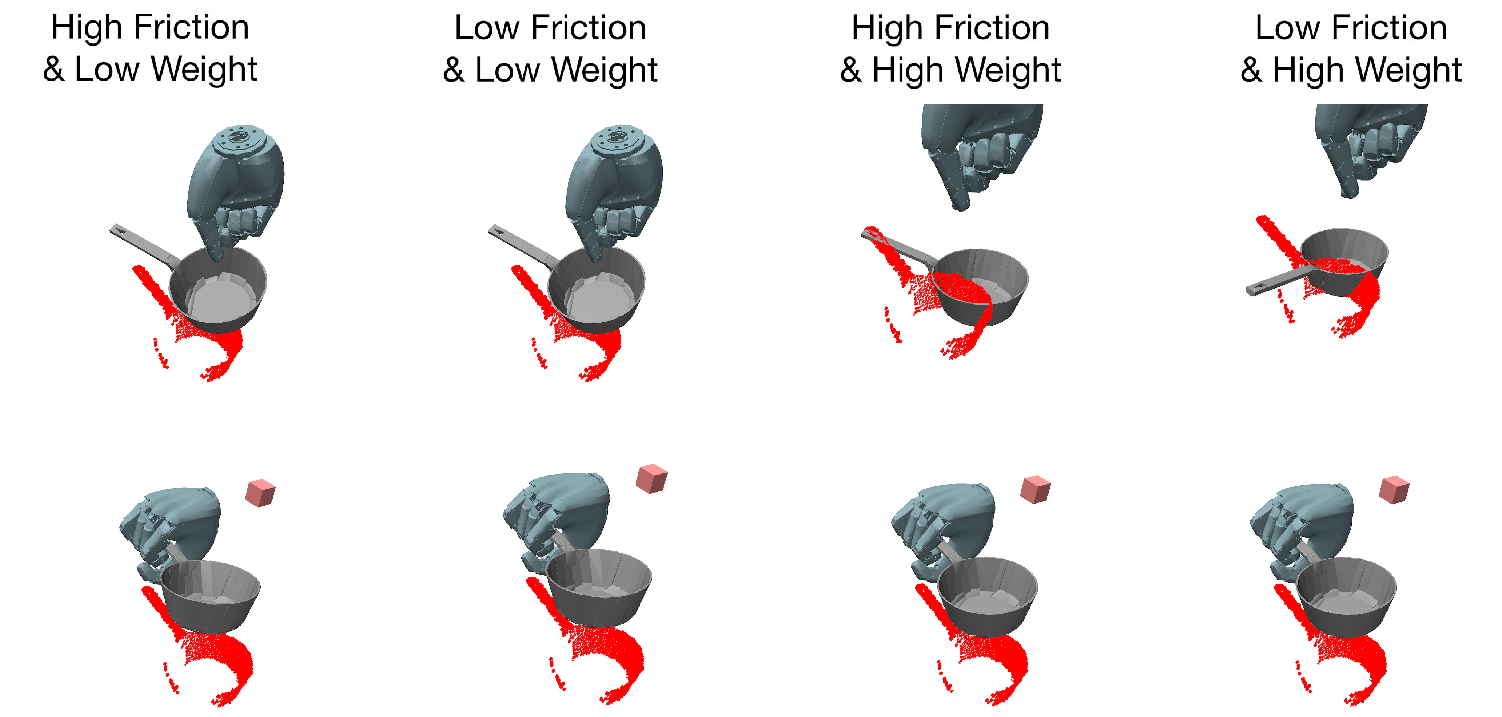
\includegraphics[width=\columnwidth]{images/frictionweight}
%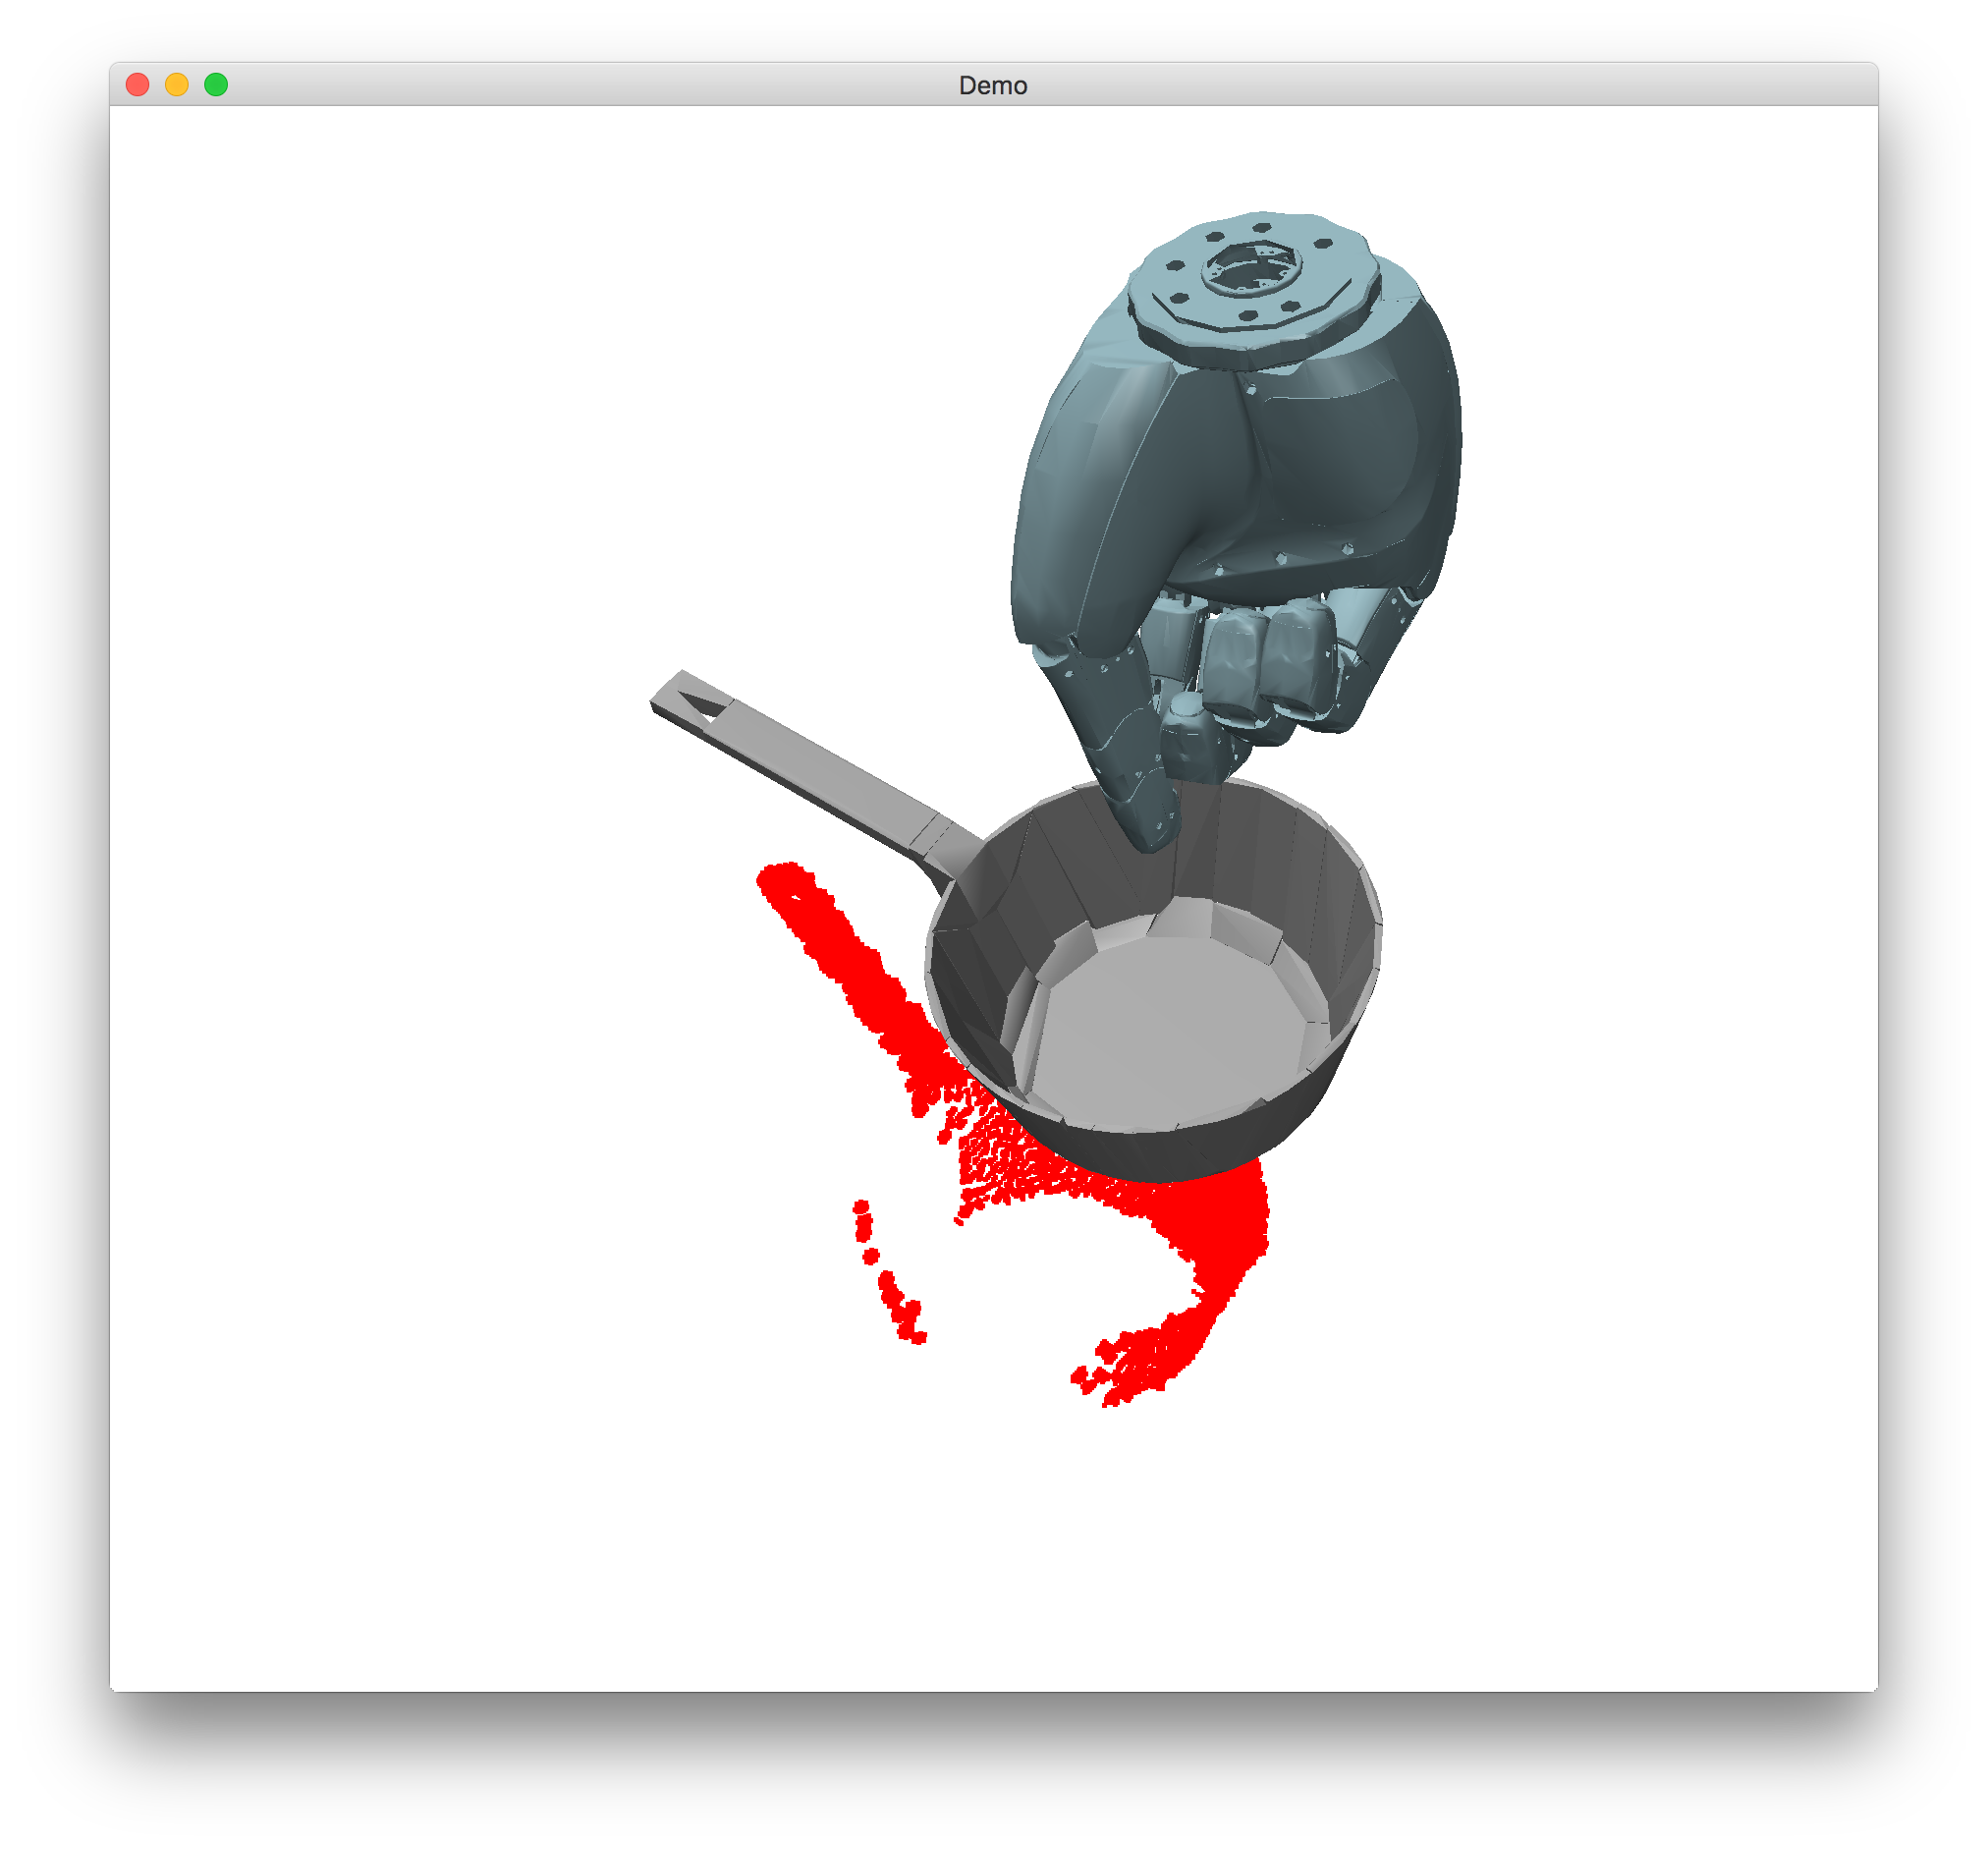
\includegraphics[width=0.24\textwidth]{images/Pan4_2_HFLW}
%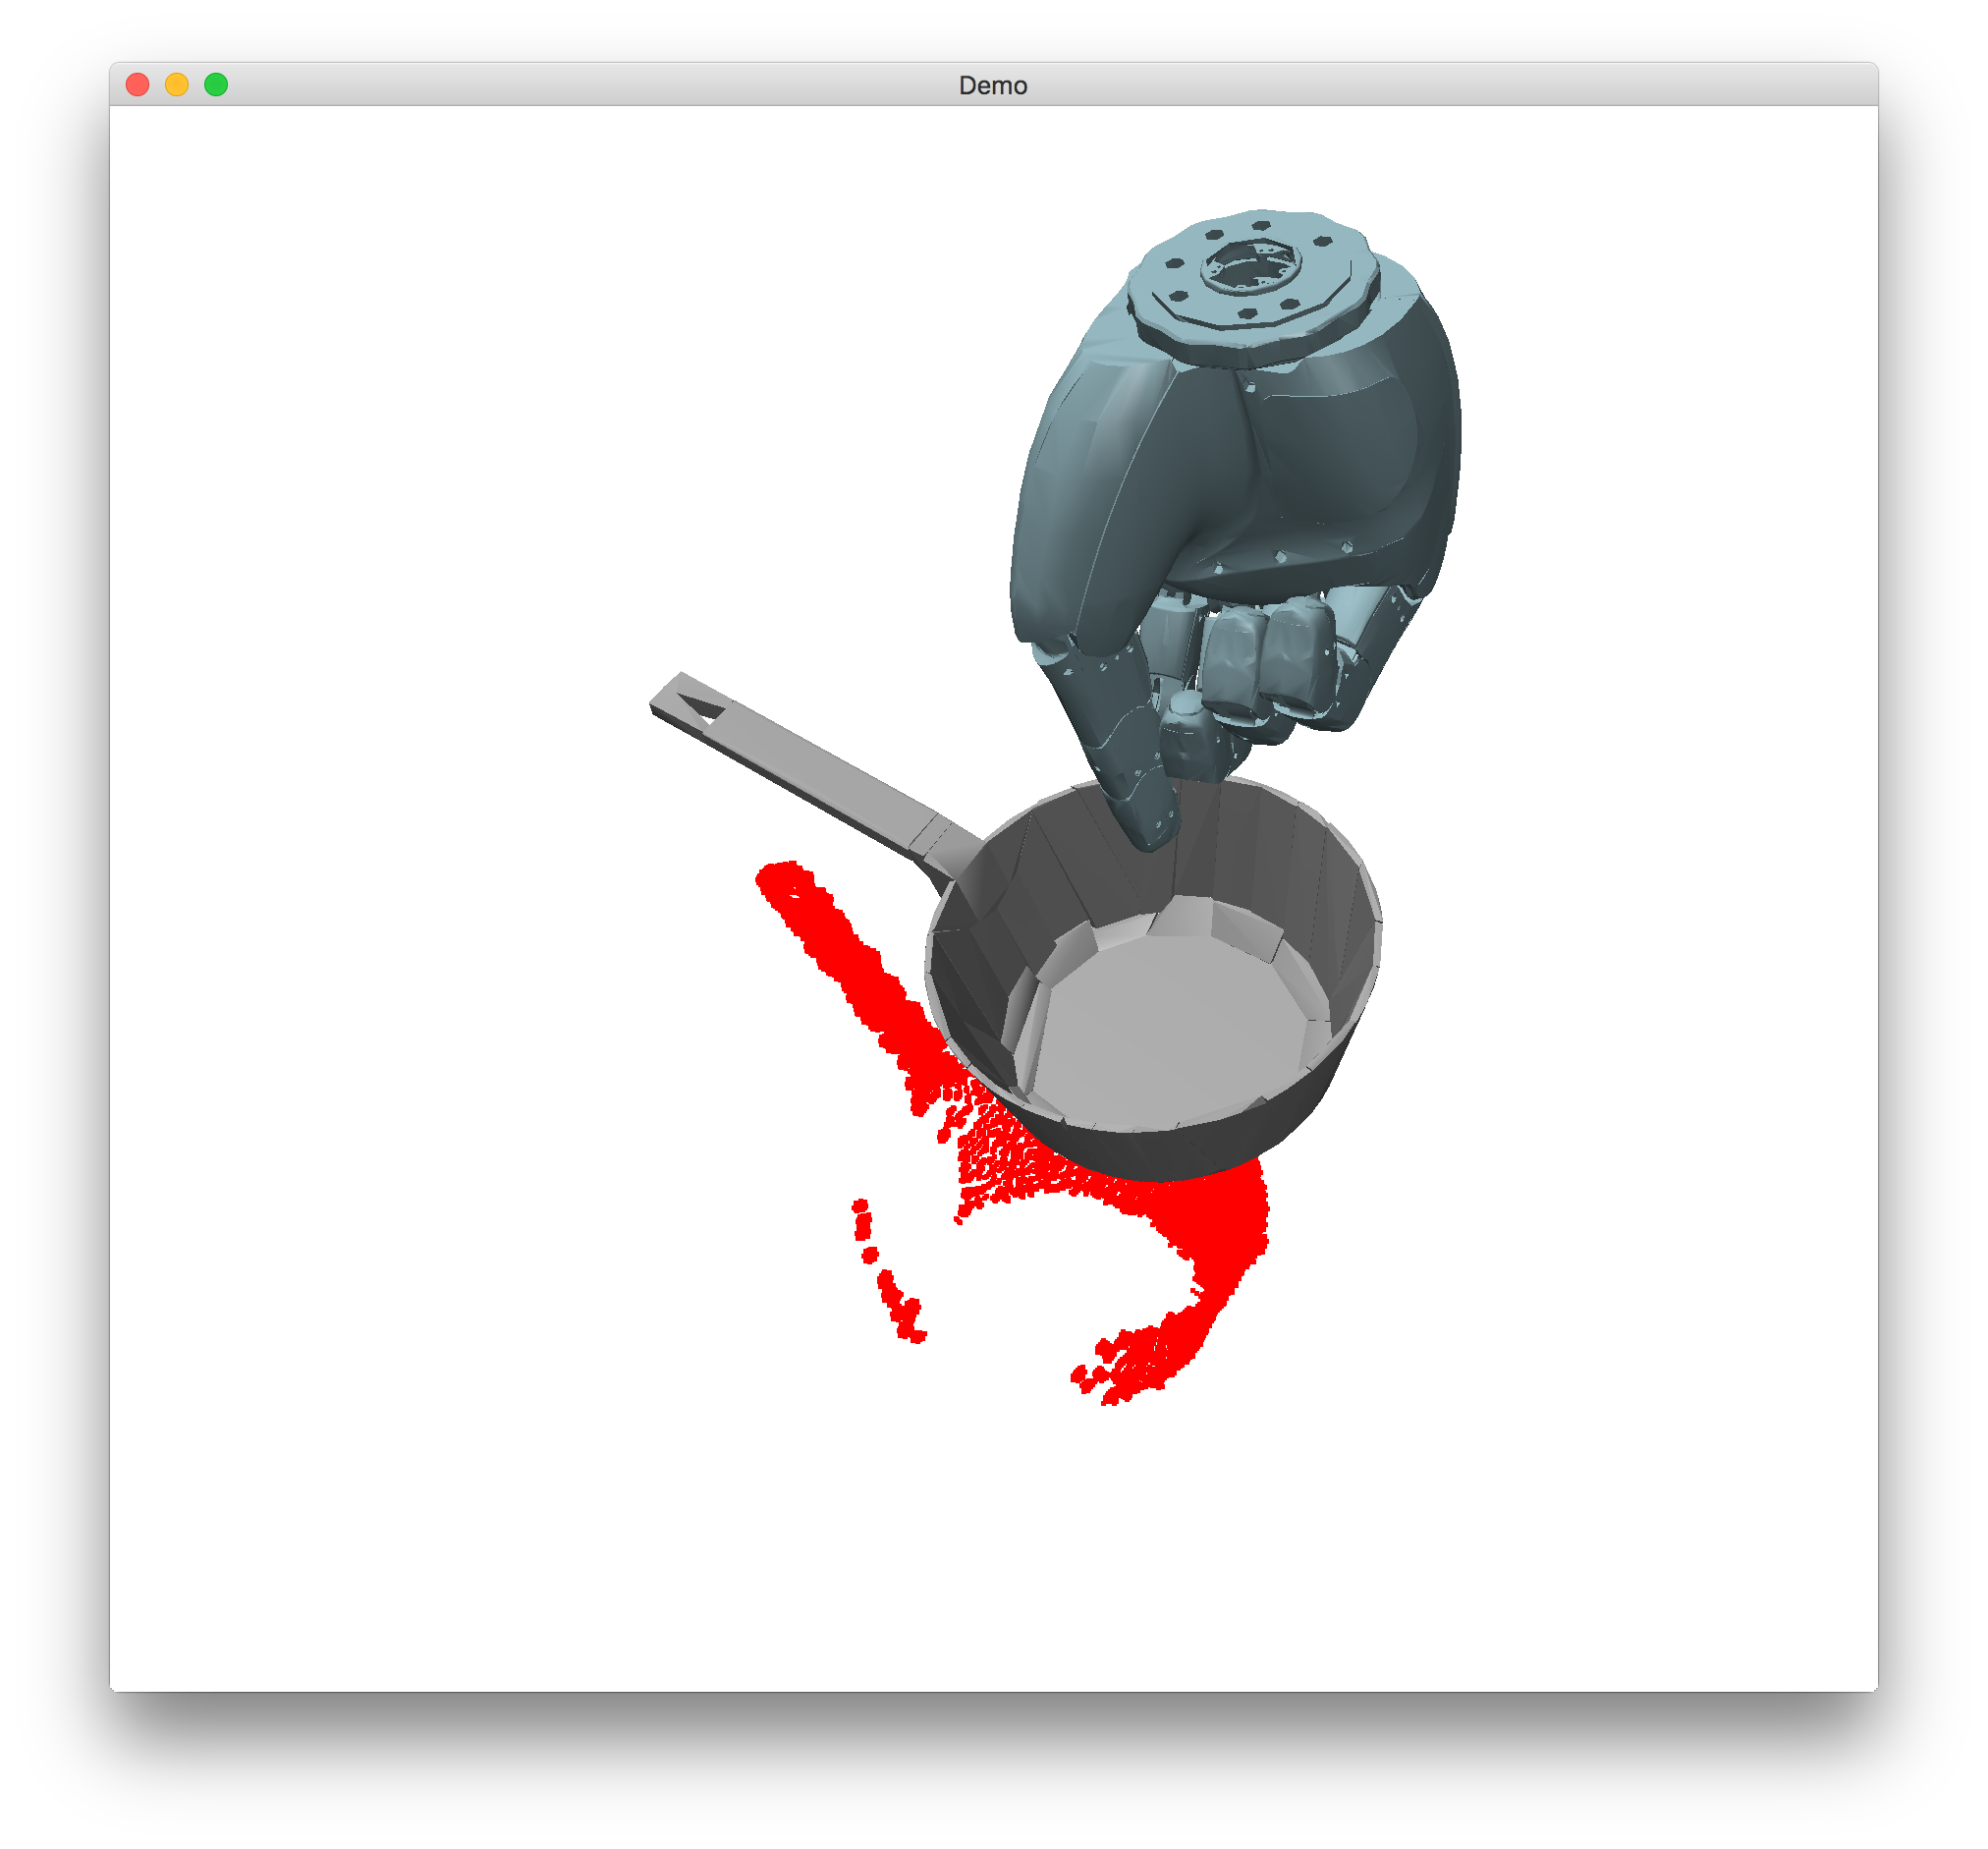
\includegraphics[width=0.24\textwidth]{images/Pan4_2_LFLW}
%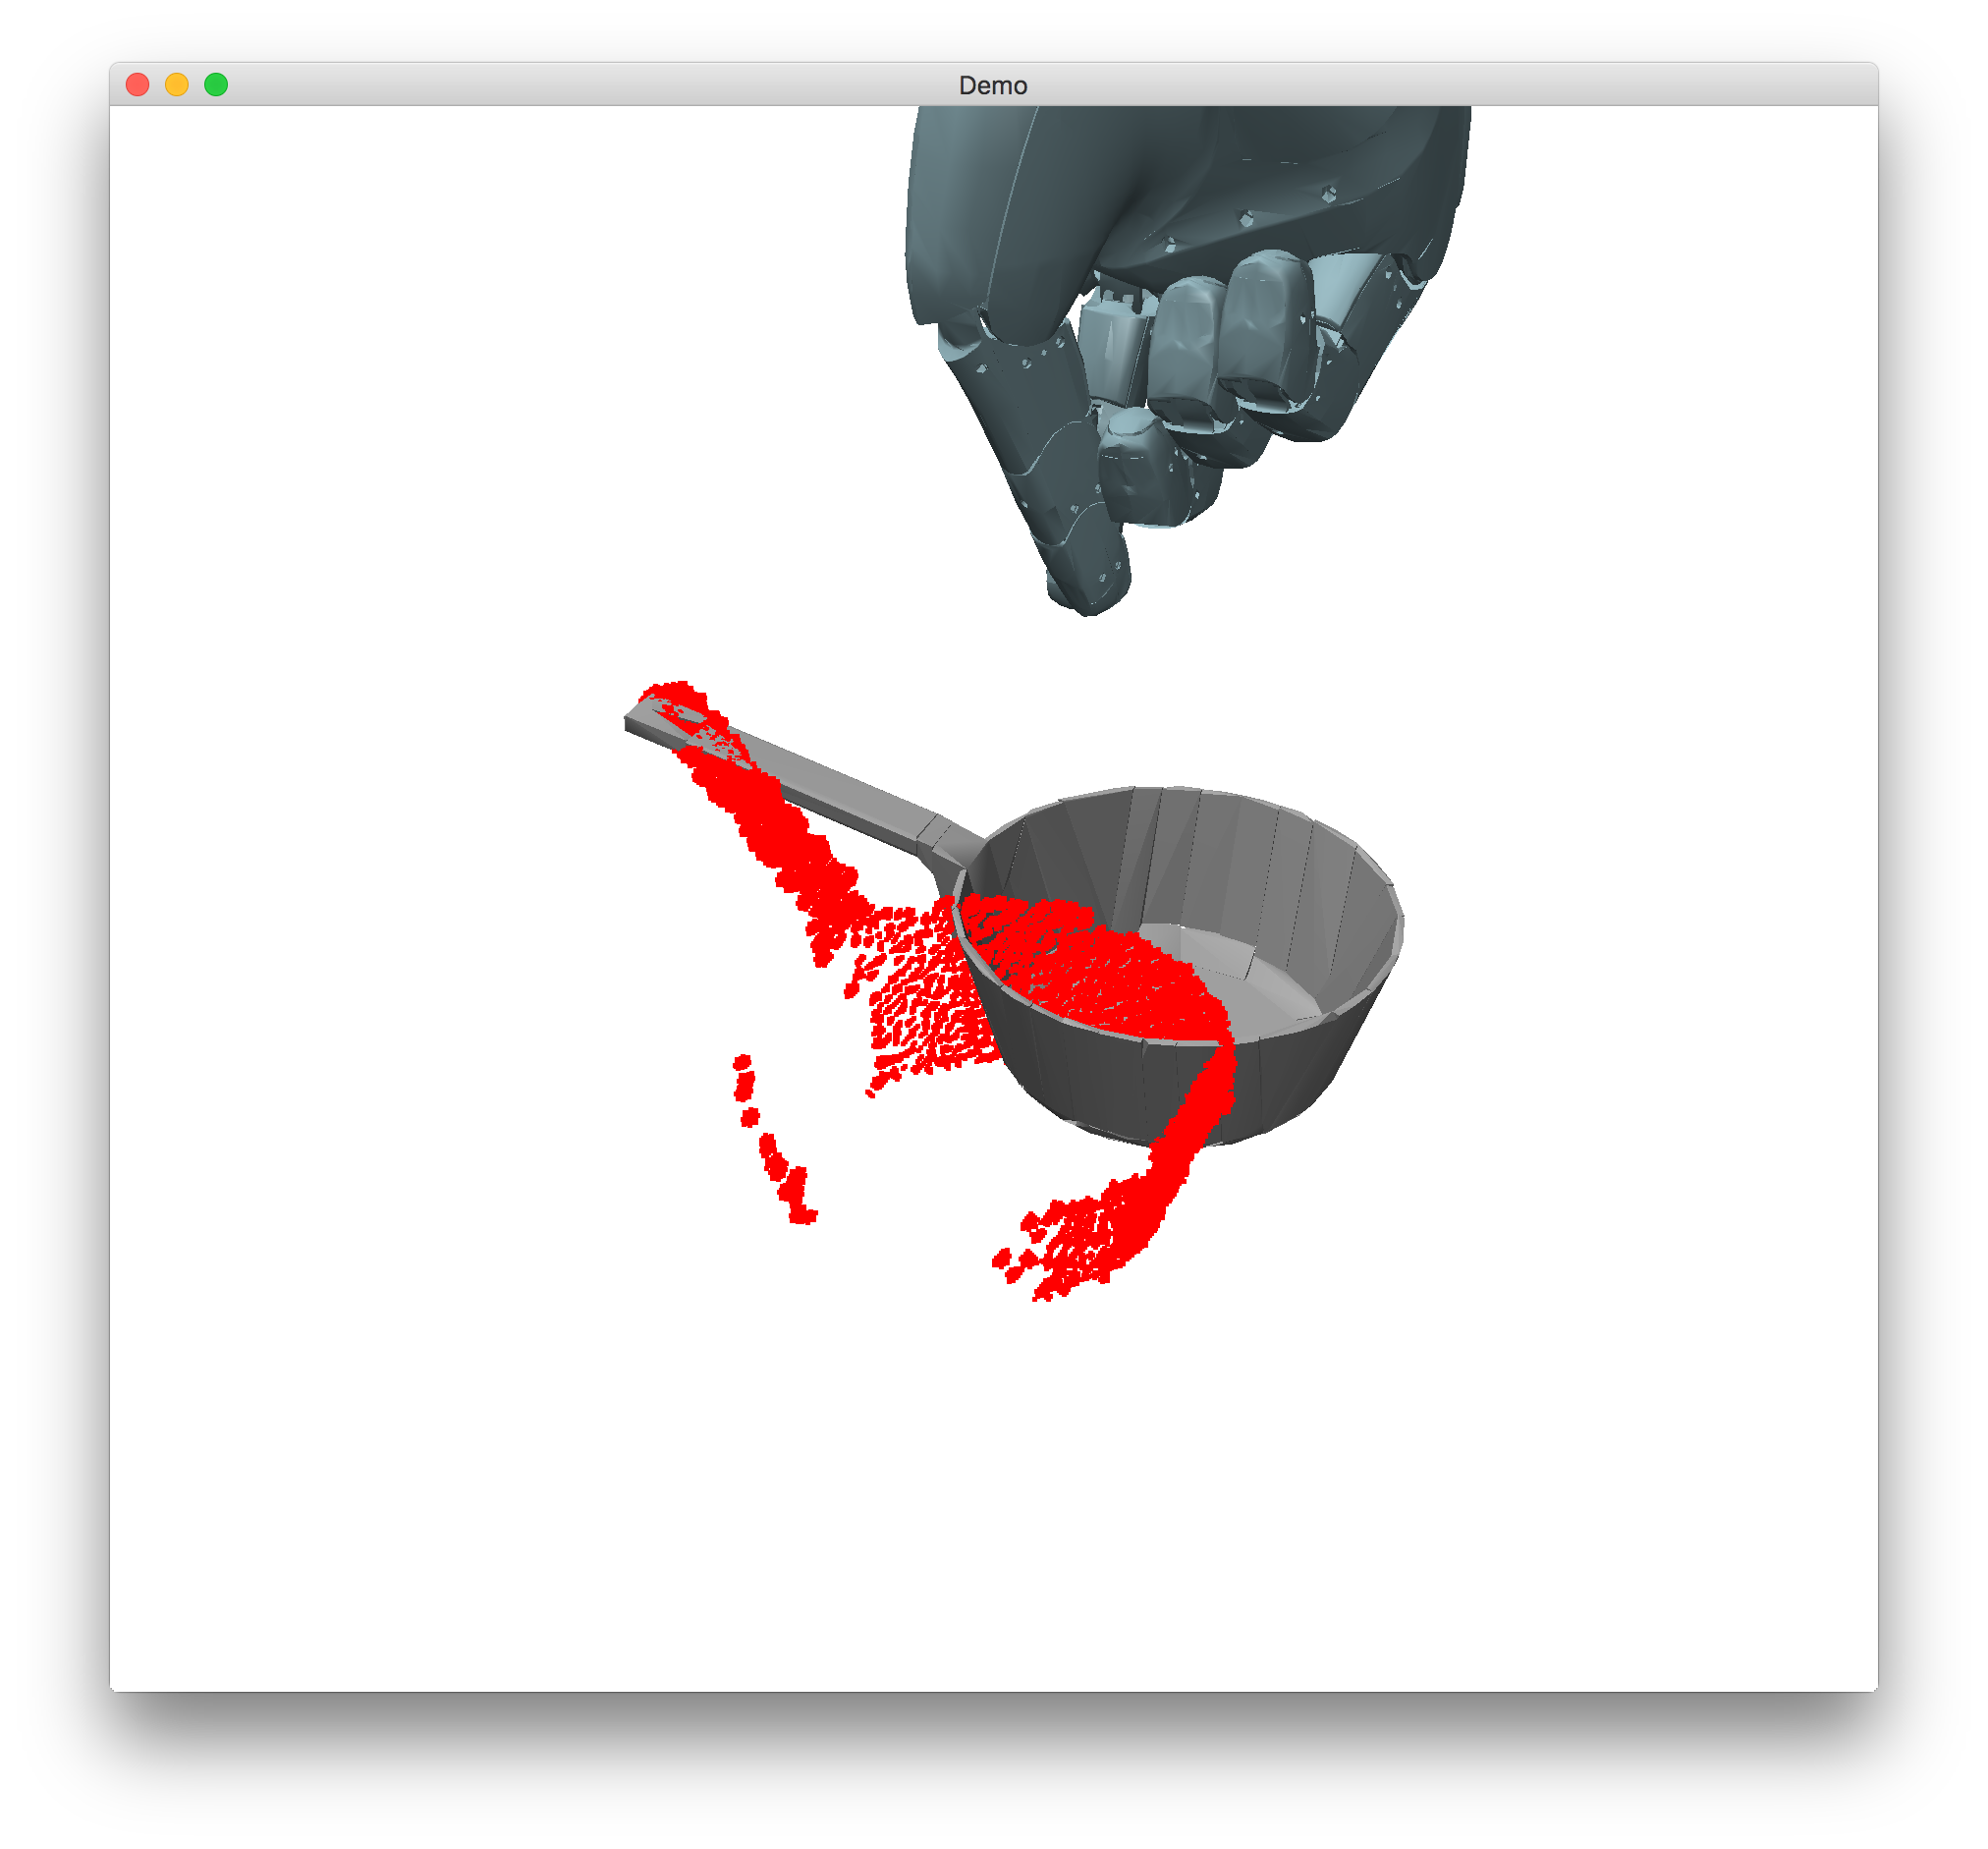
\includegraphics[width=0.24\textwidth]{images/Pan4_2_HFHW}
%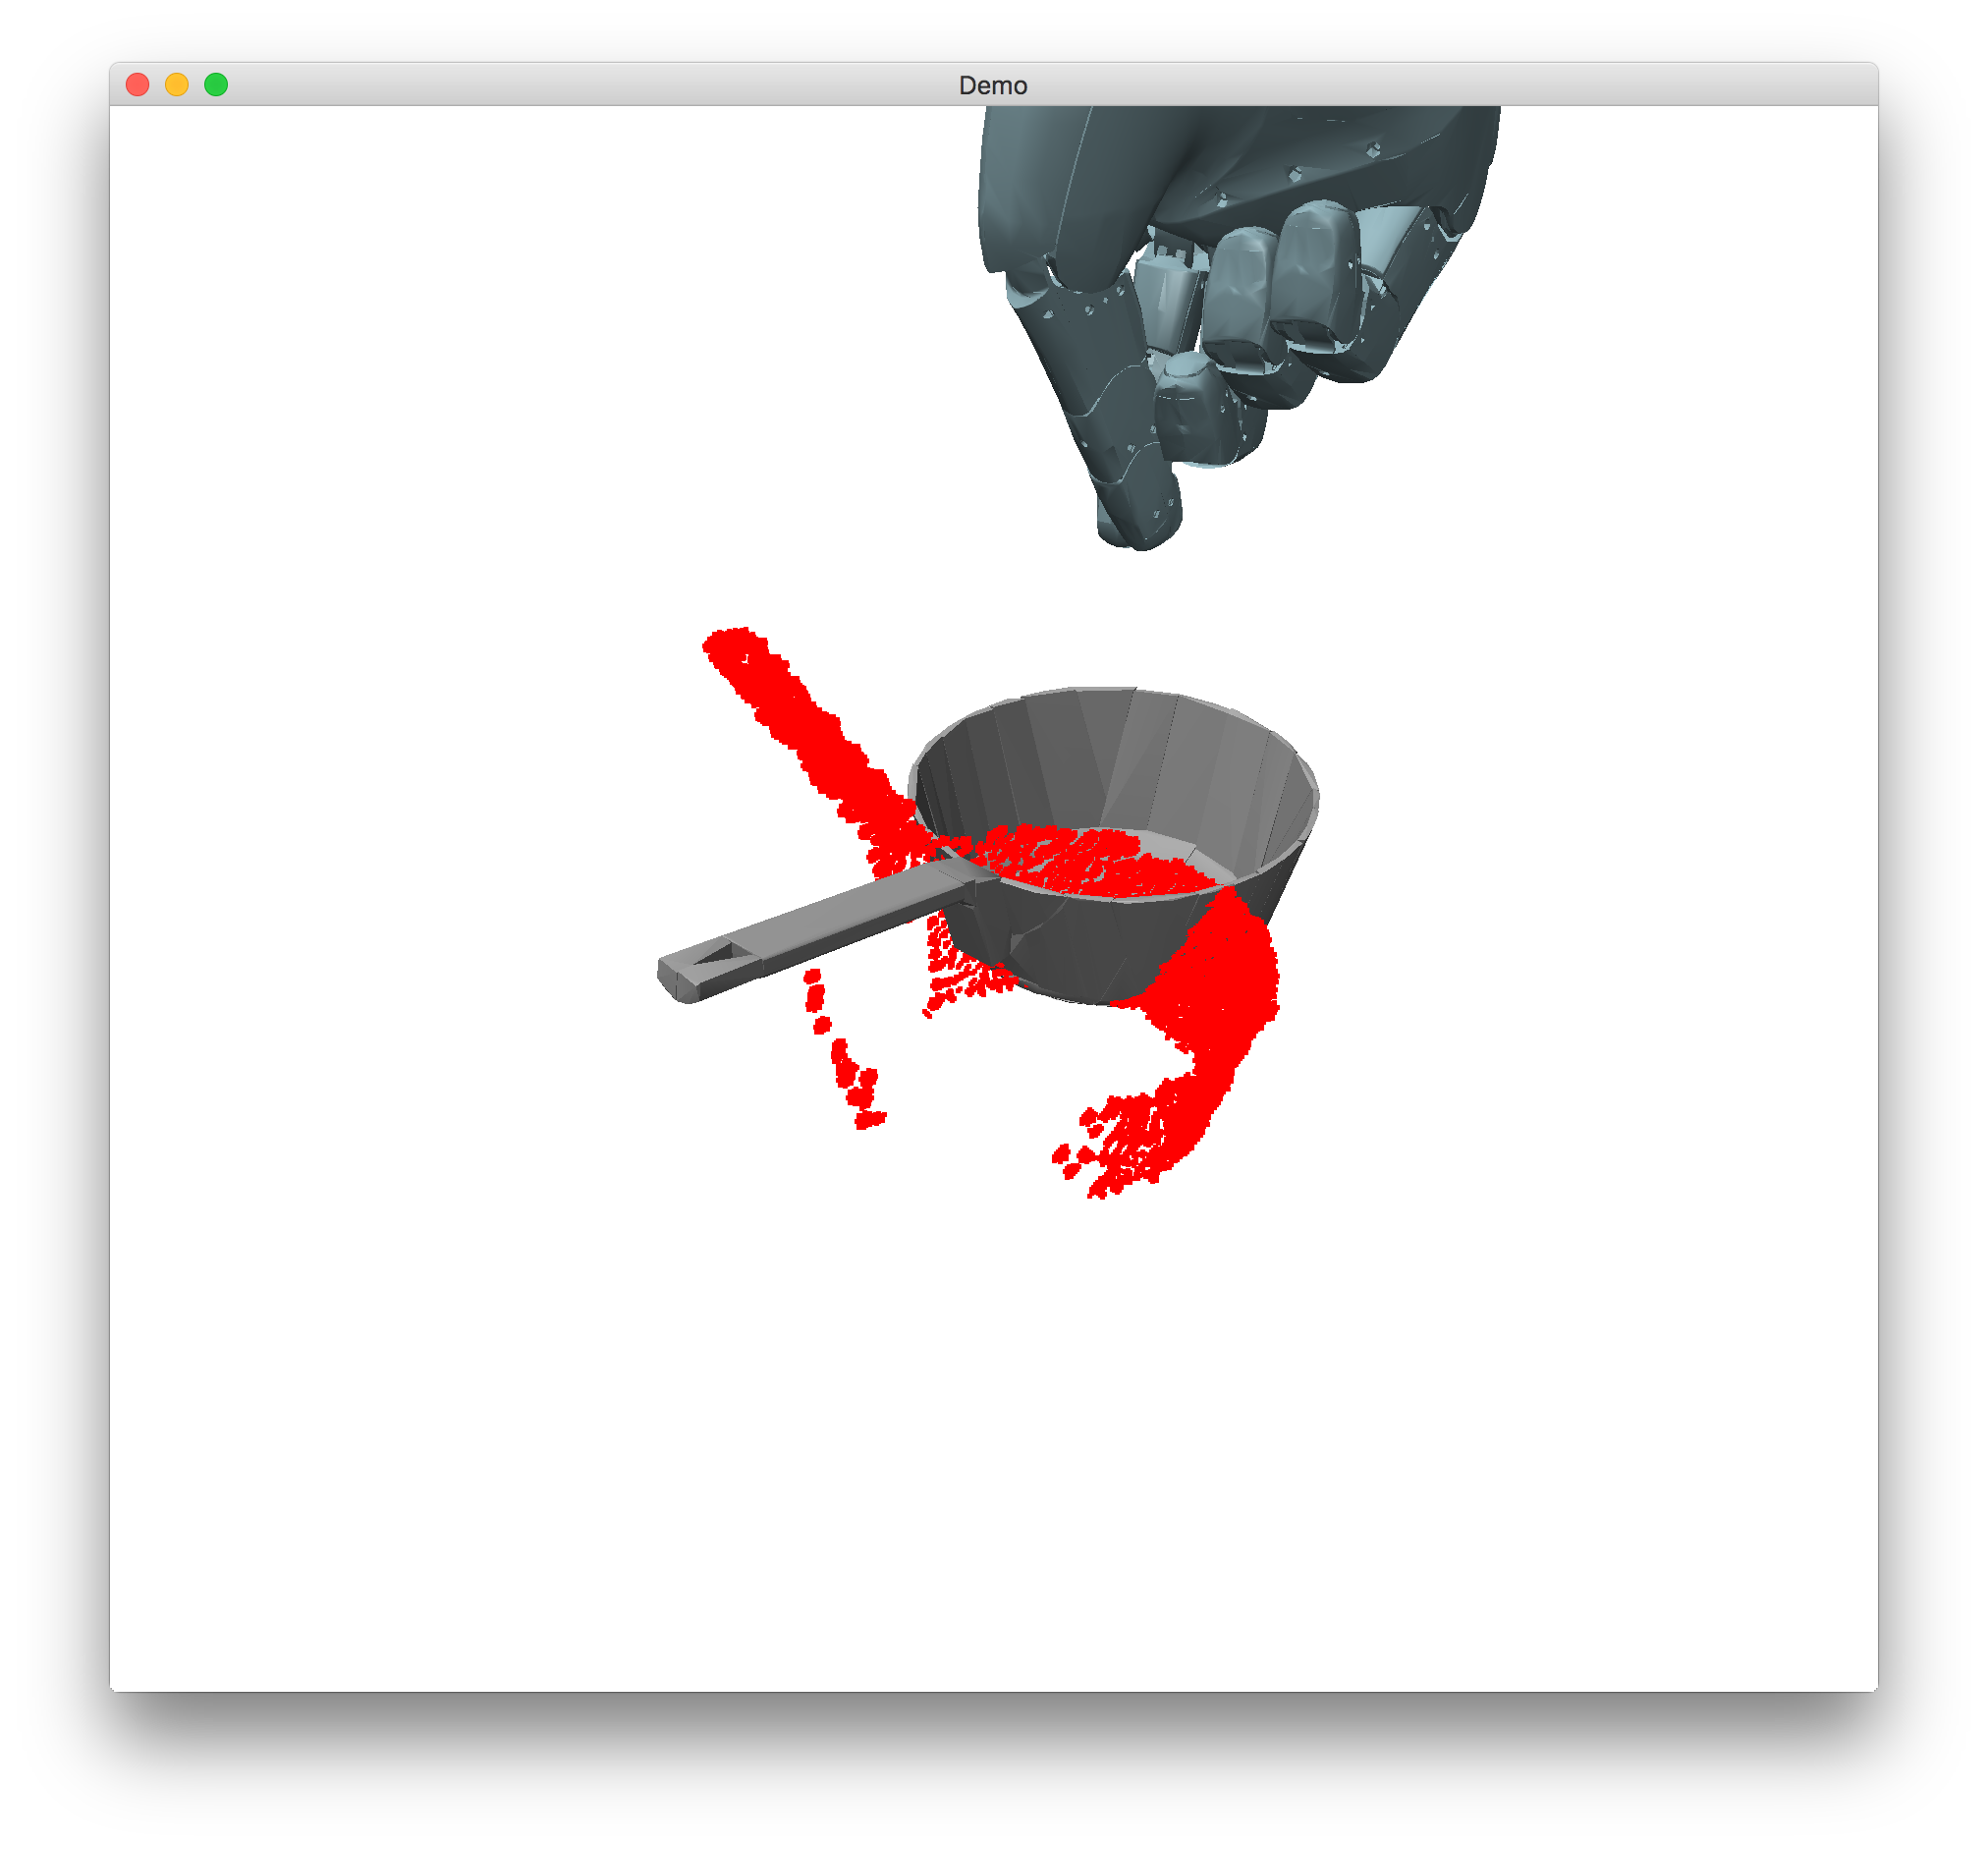
\includegraphics[width=0.24\textwidth]{images/Pan4_2_LFHW}\\
%%
\includegraphics[width=0.96\textwidth]{images/key-to-eval-training}\\
%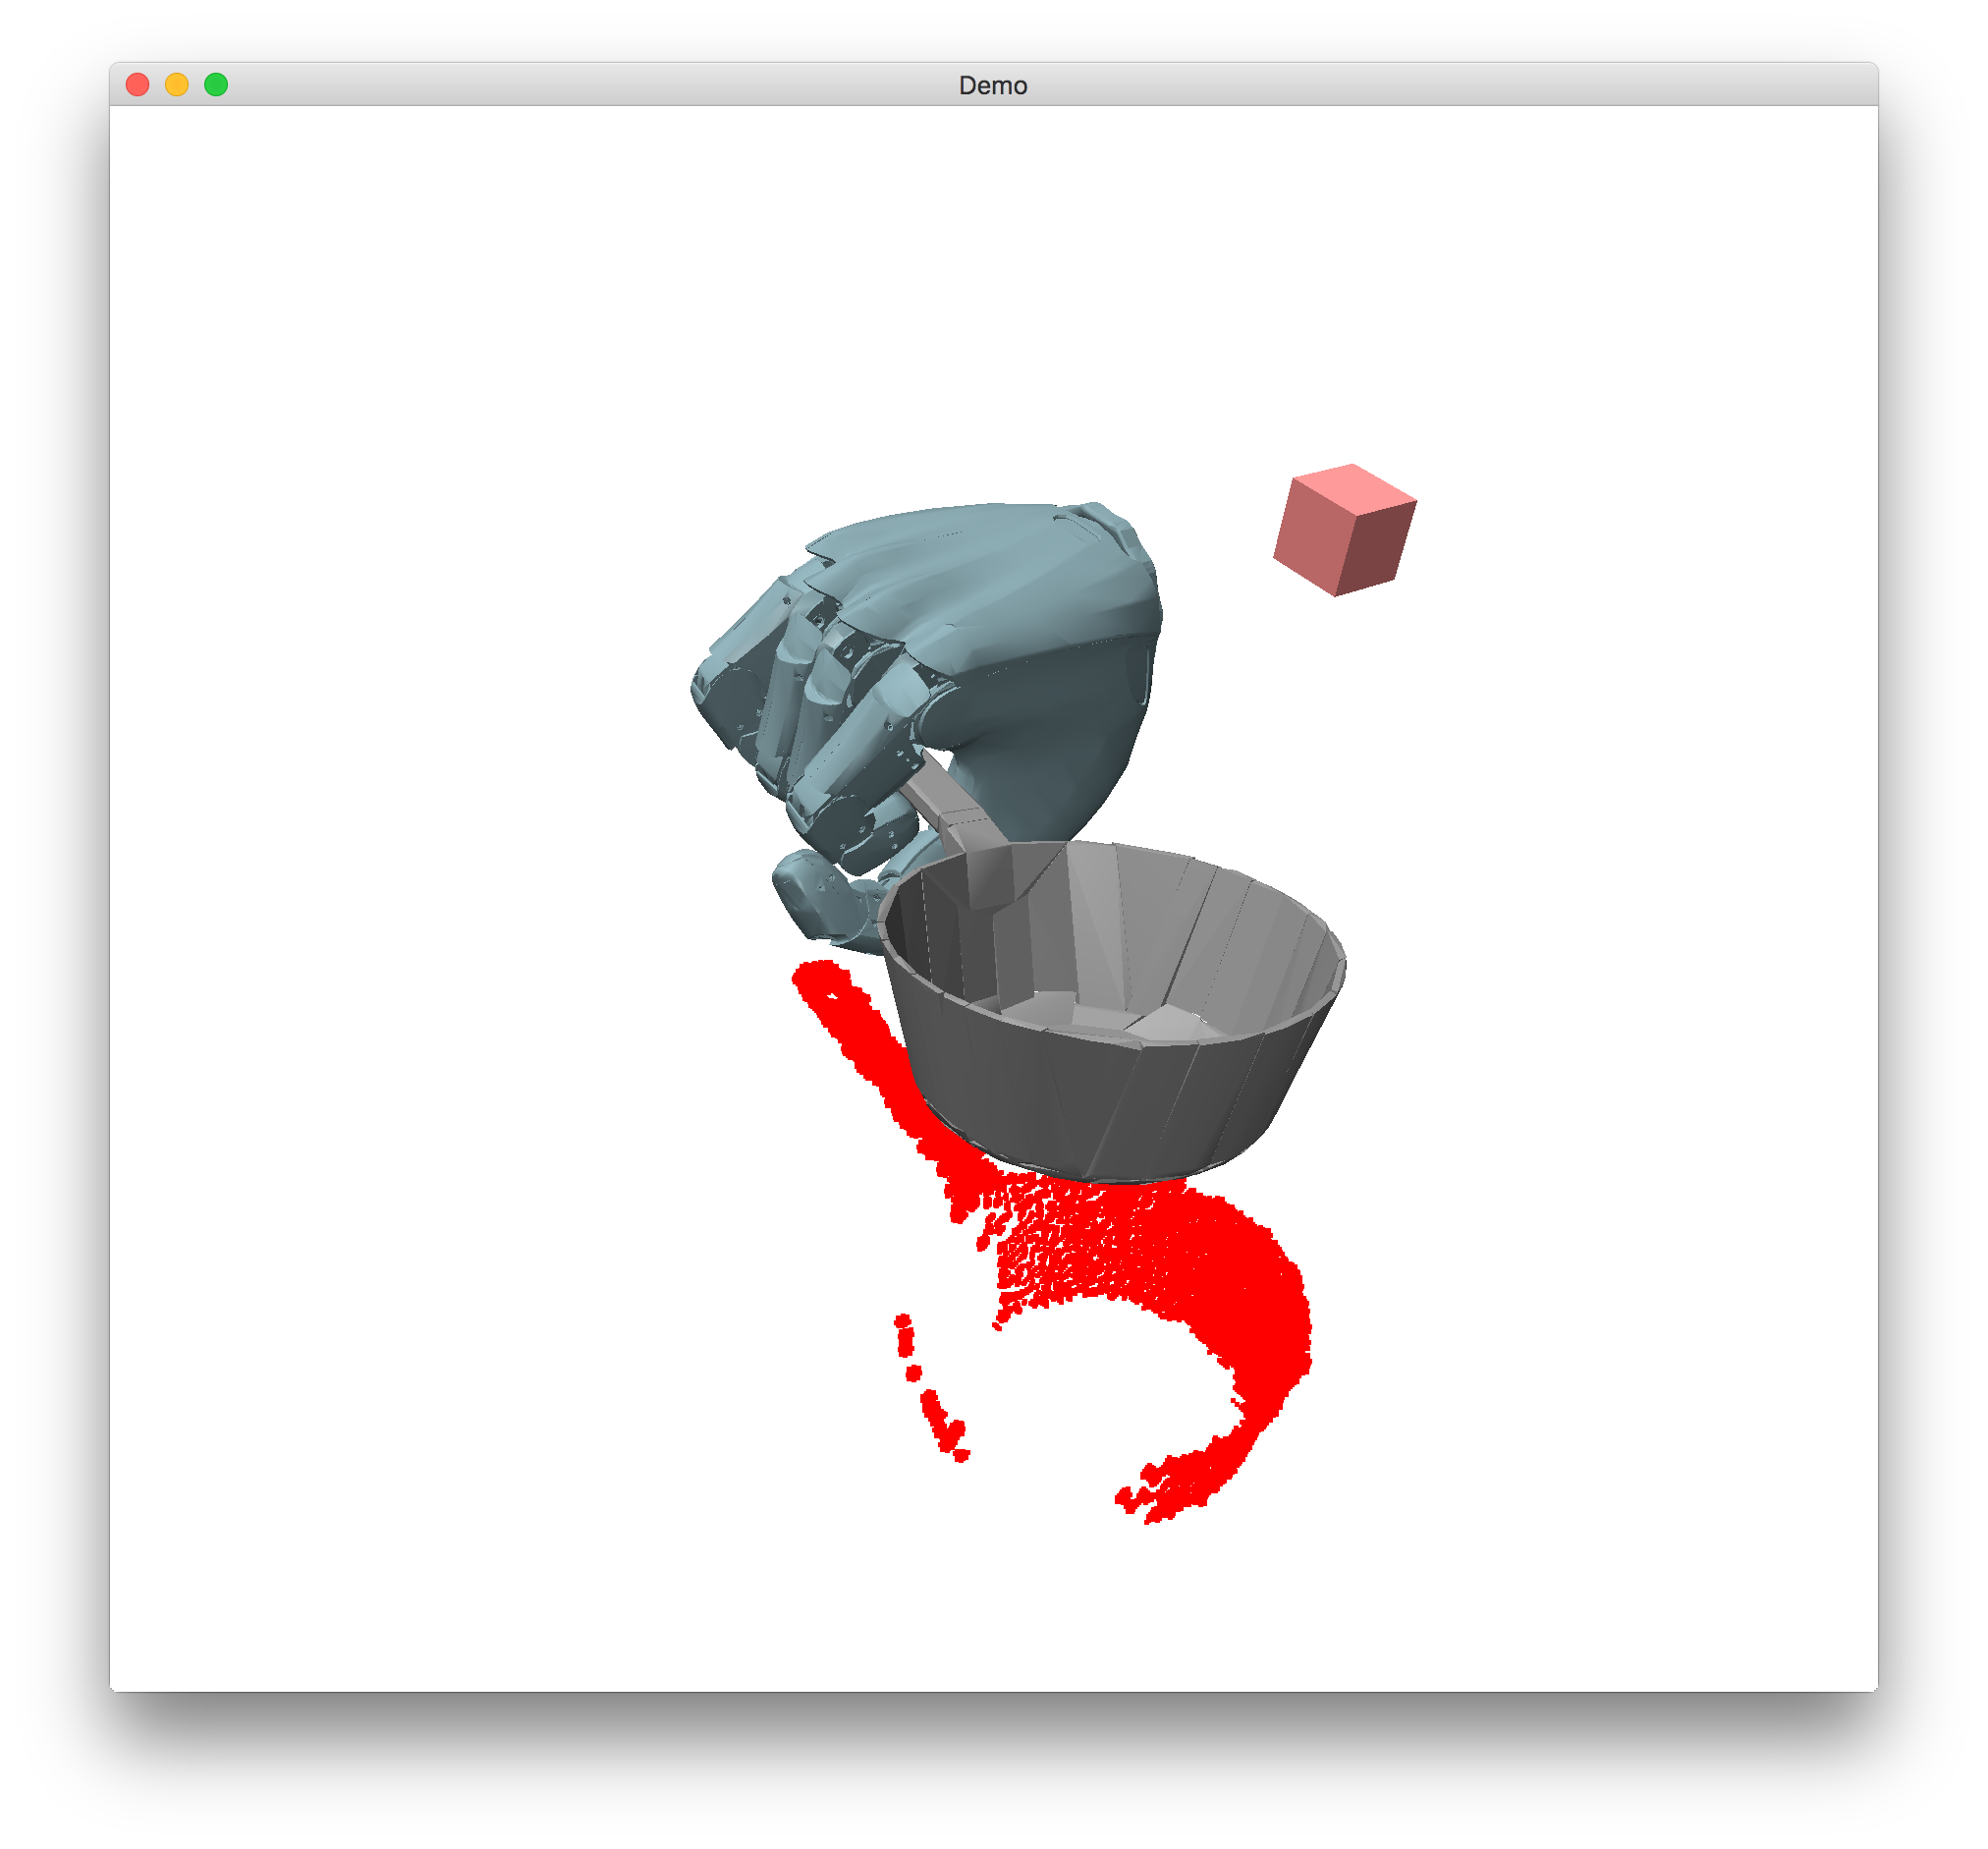
\includegraphics[width=0.24\textwidth]{images/Pan4_HFLW}
%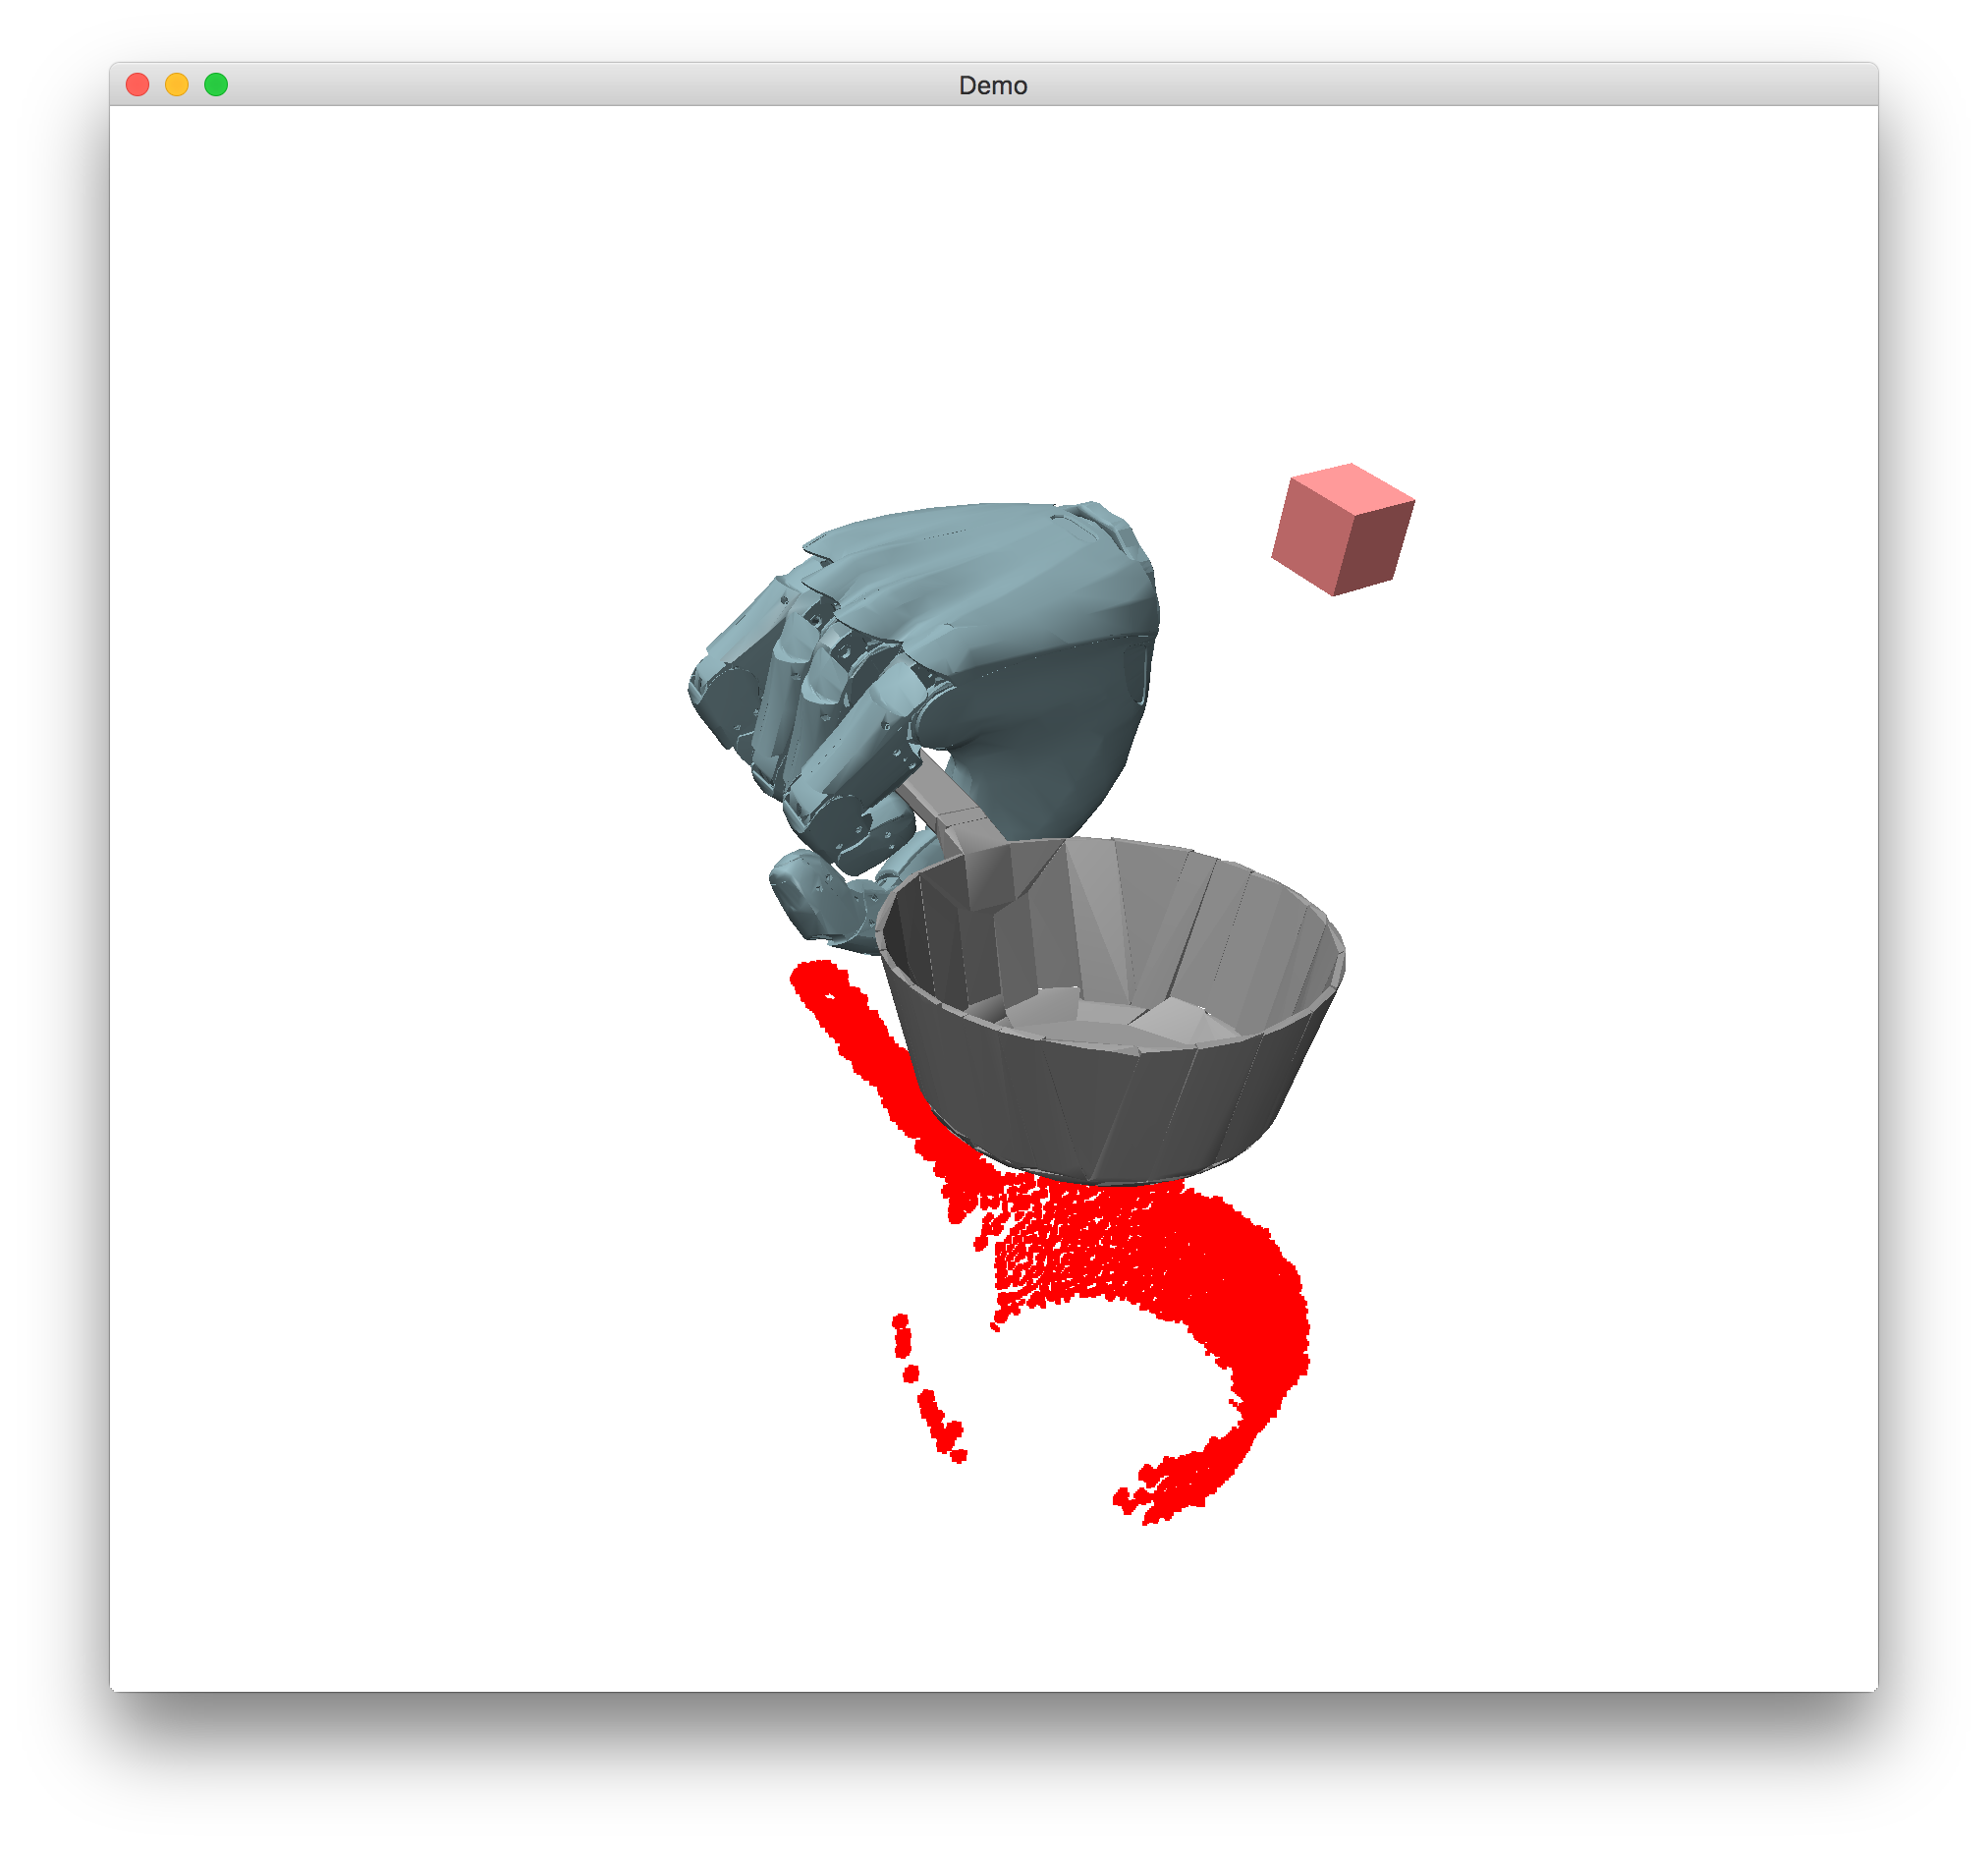
\includegraphics[width=0.24\textwidth]{images/Pan4_LFLW}
%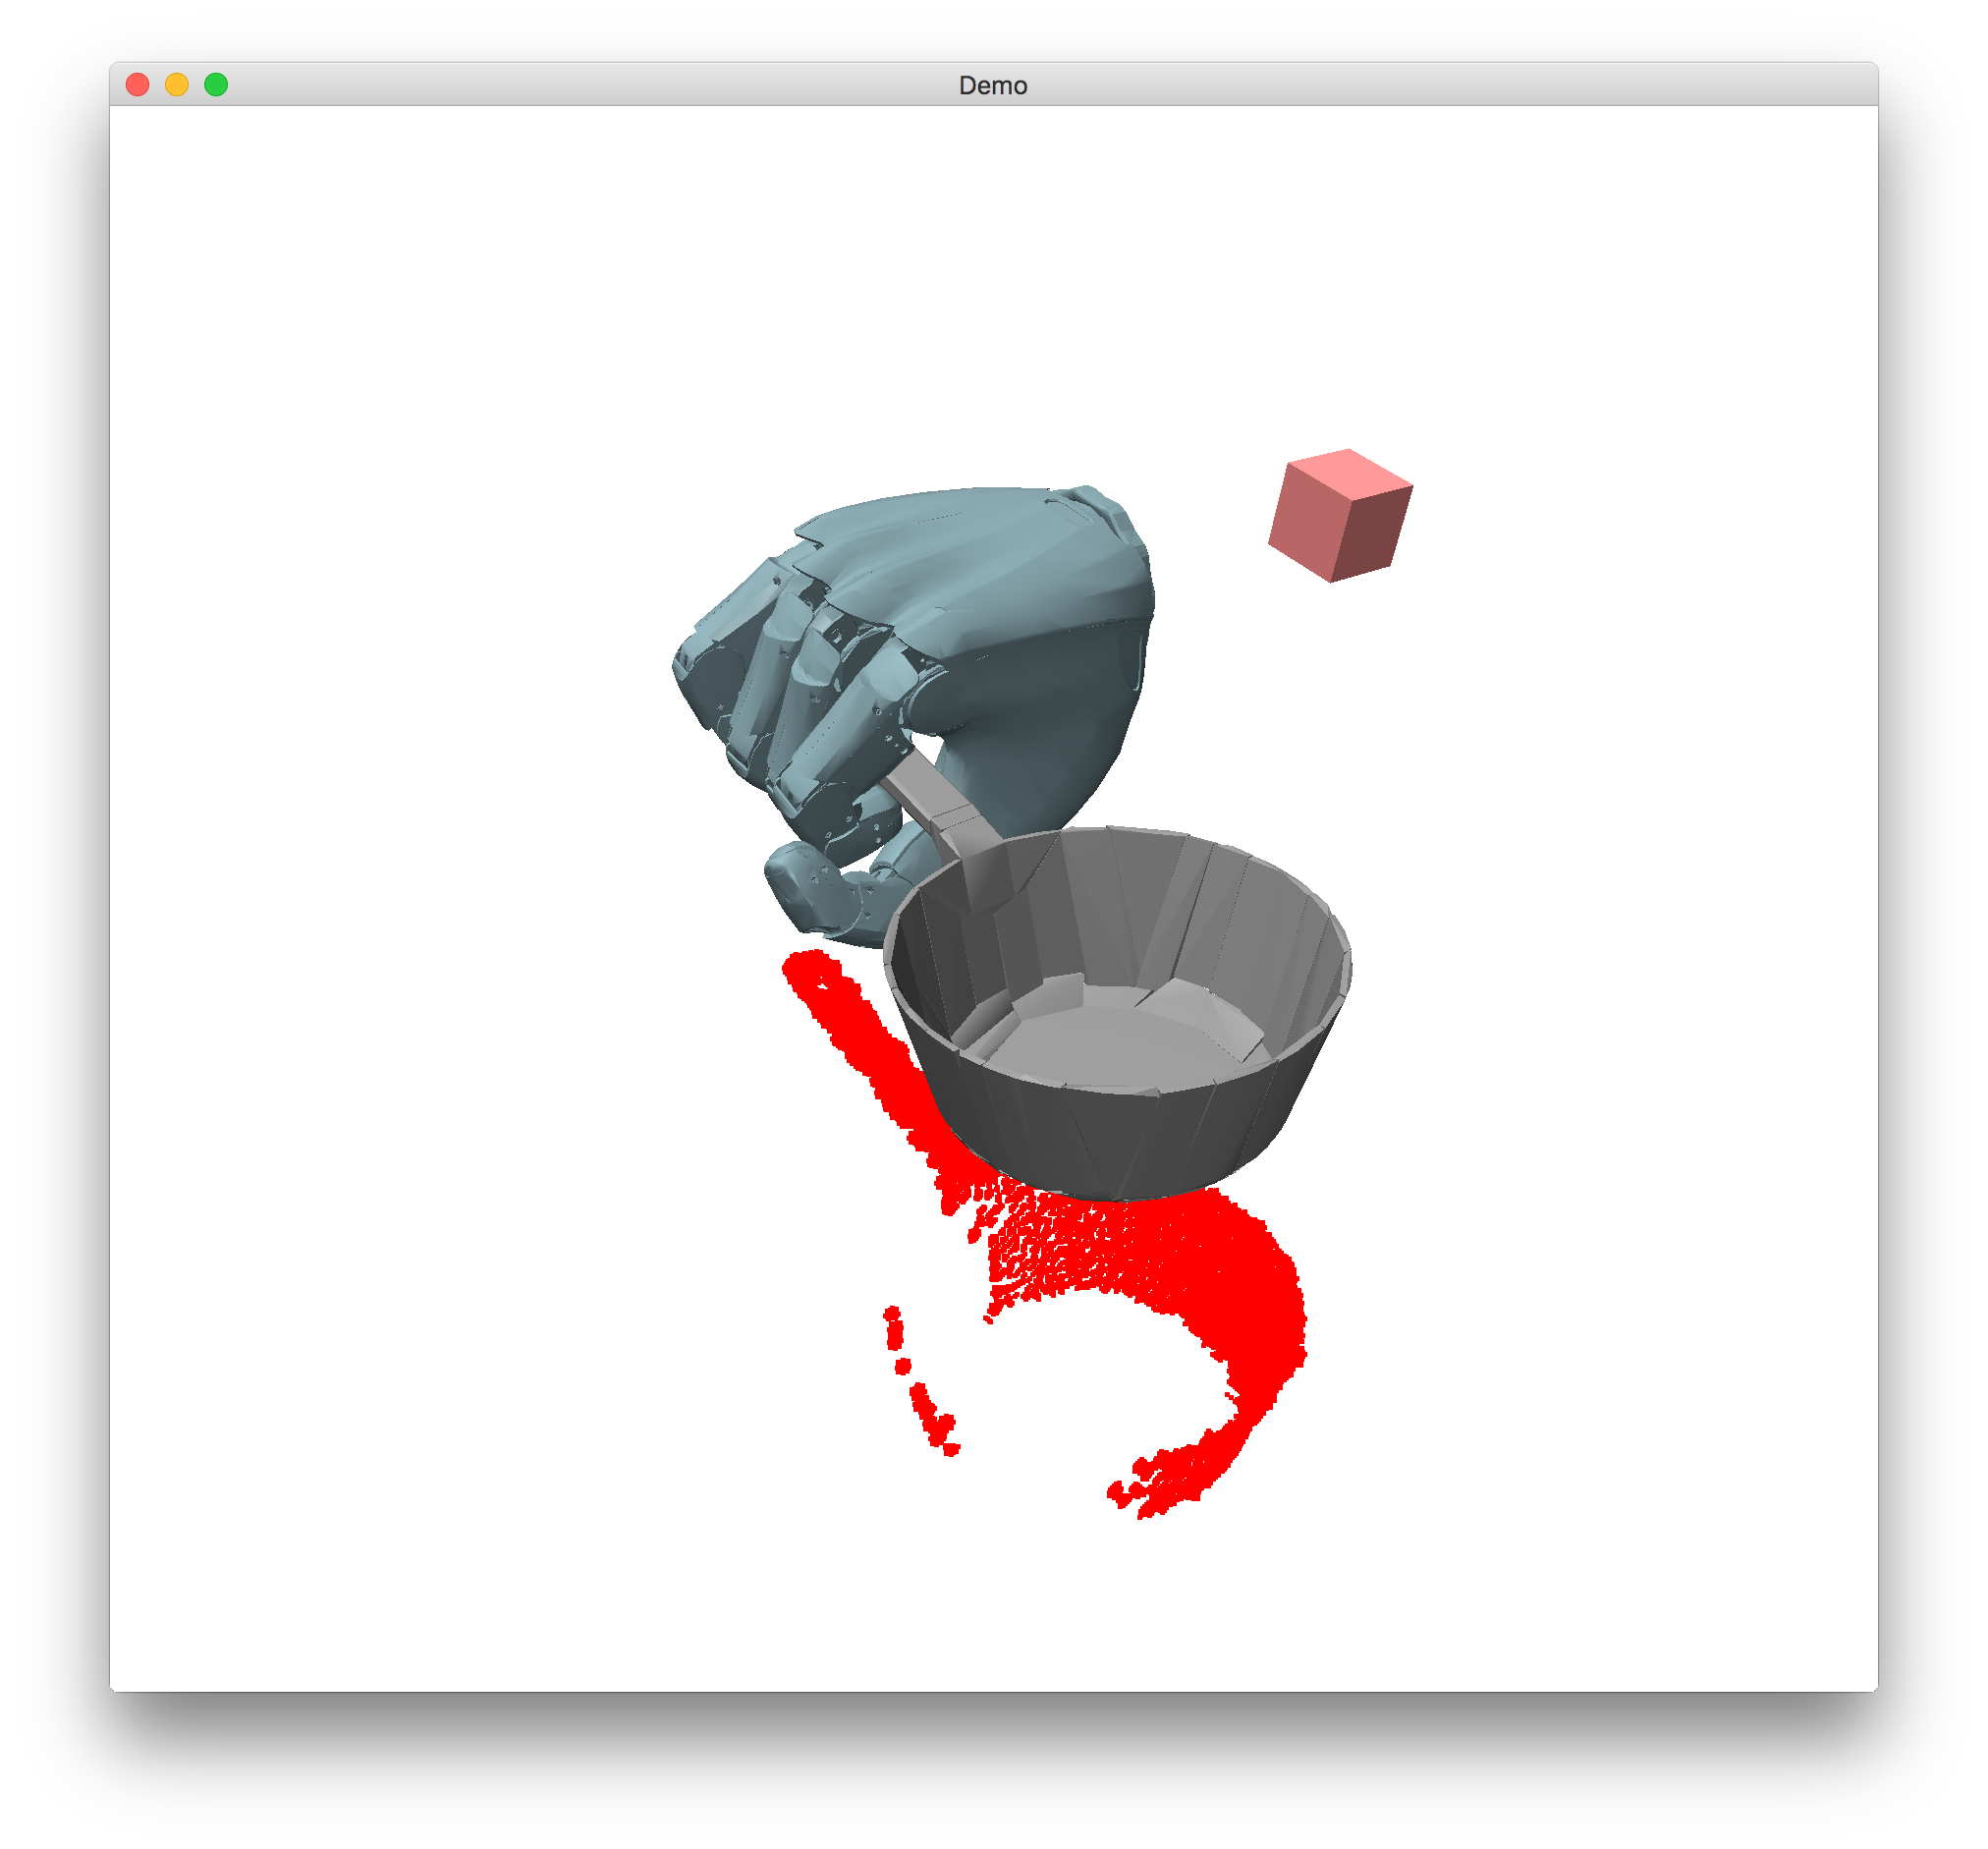
\includegraphics[width=0.24\textwidth]{images/Pan4_HFHW}
%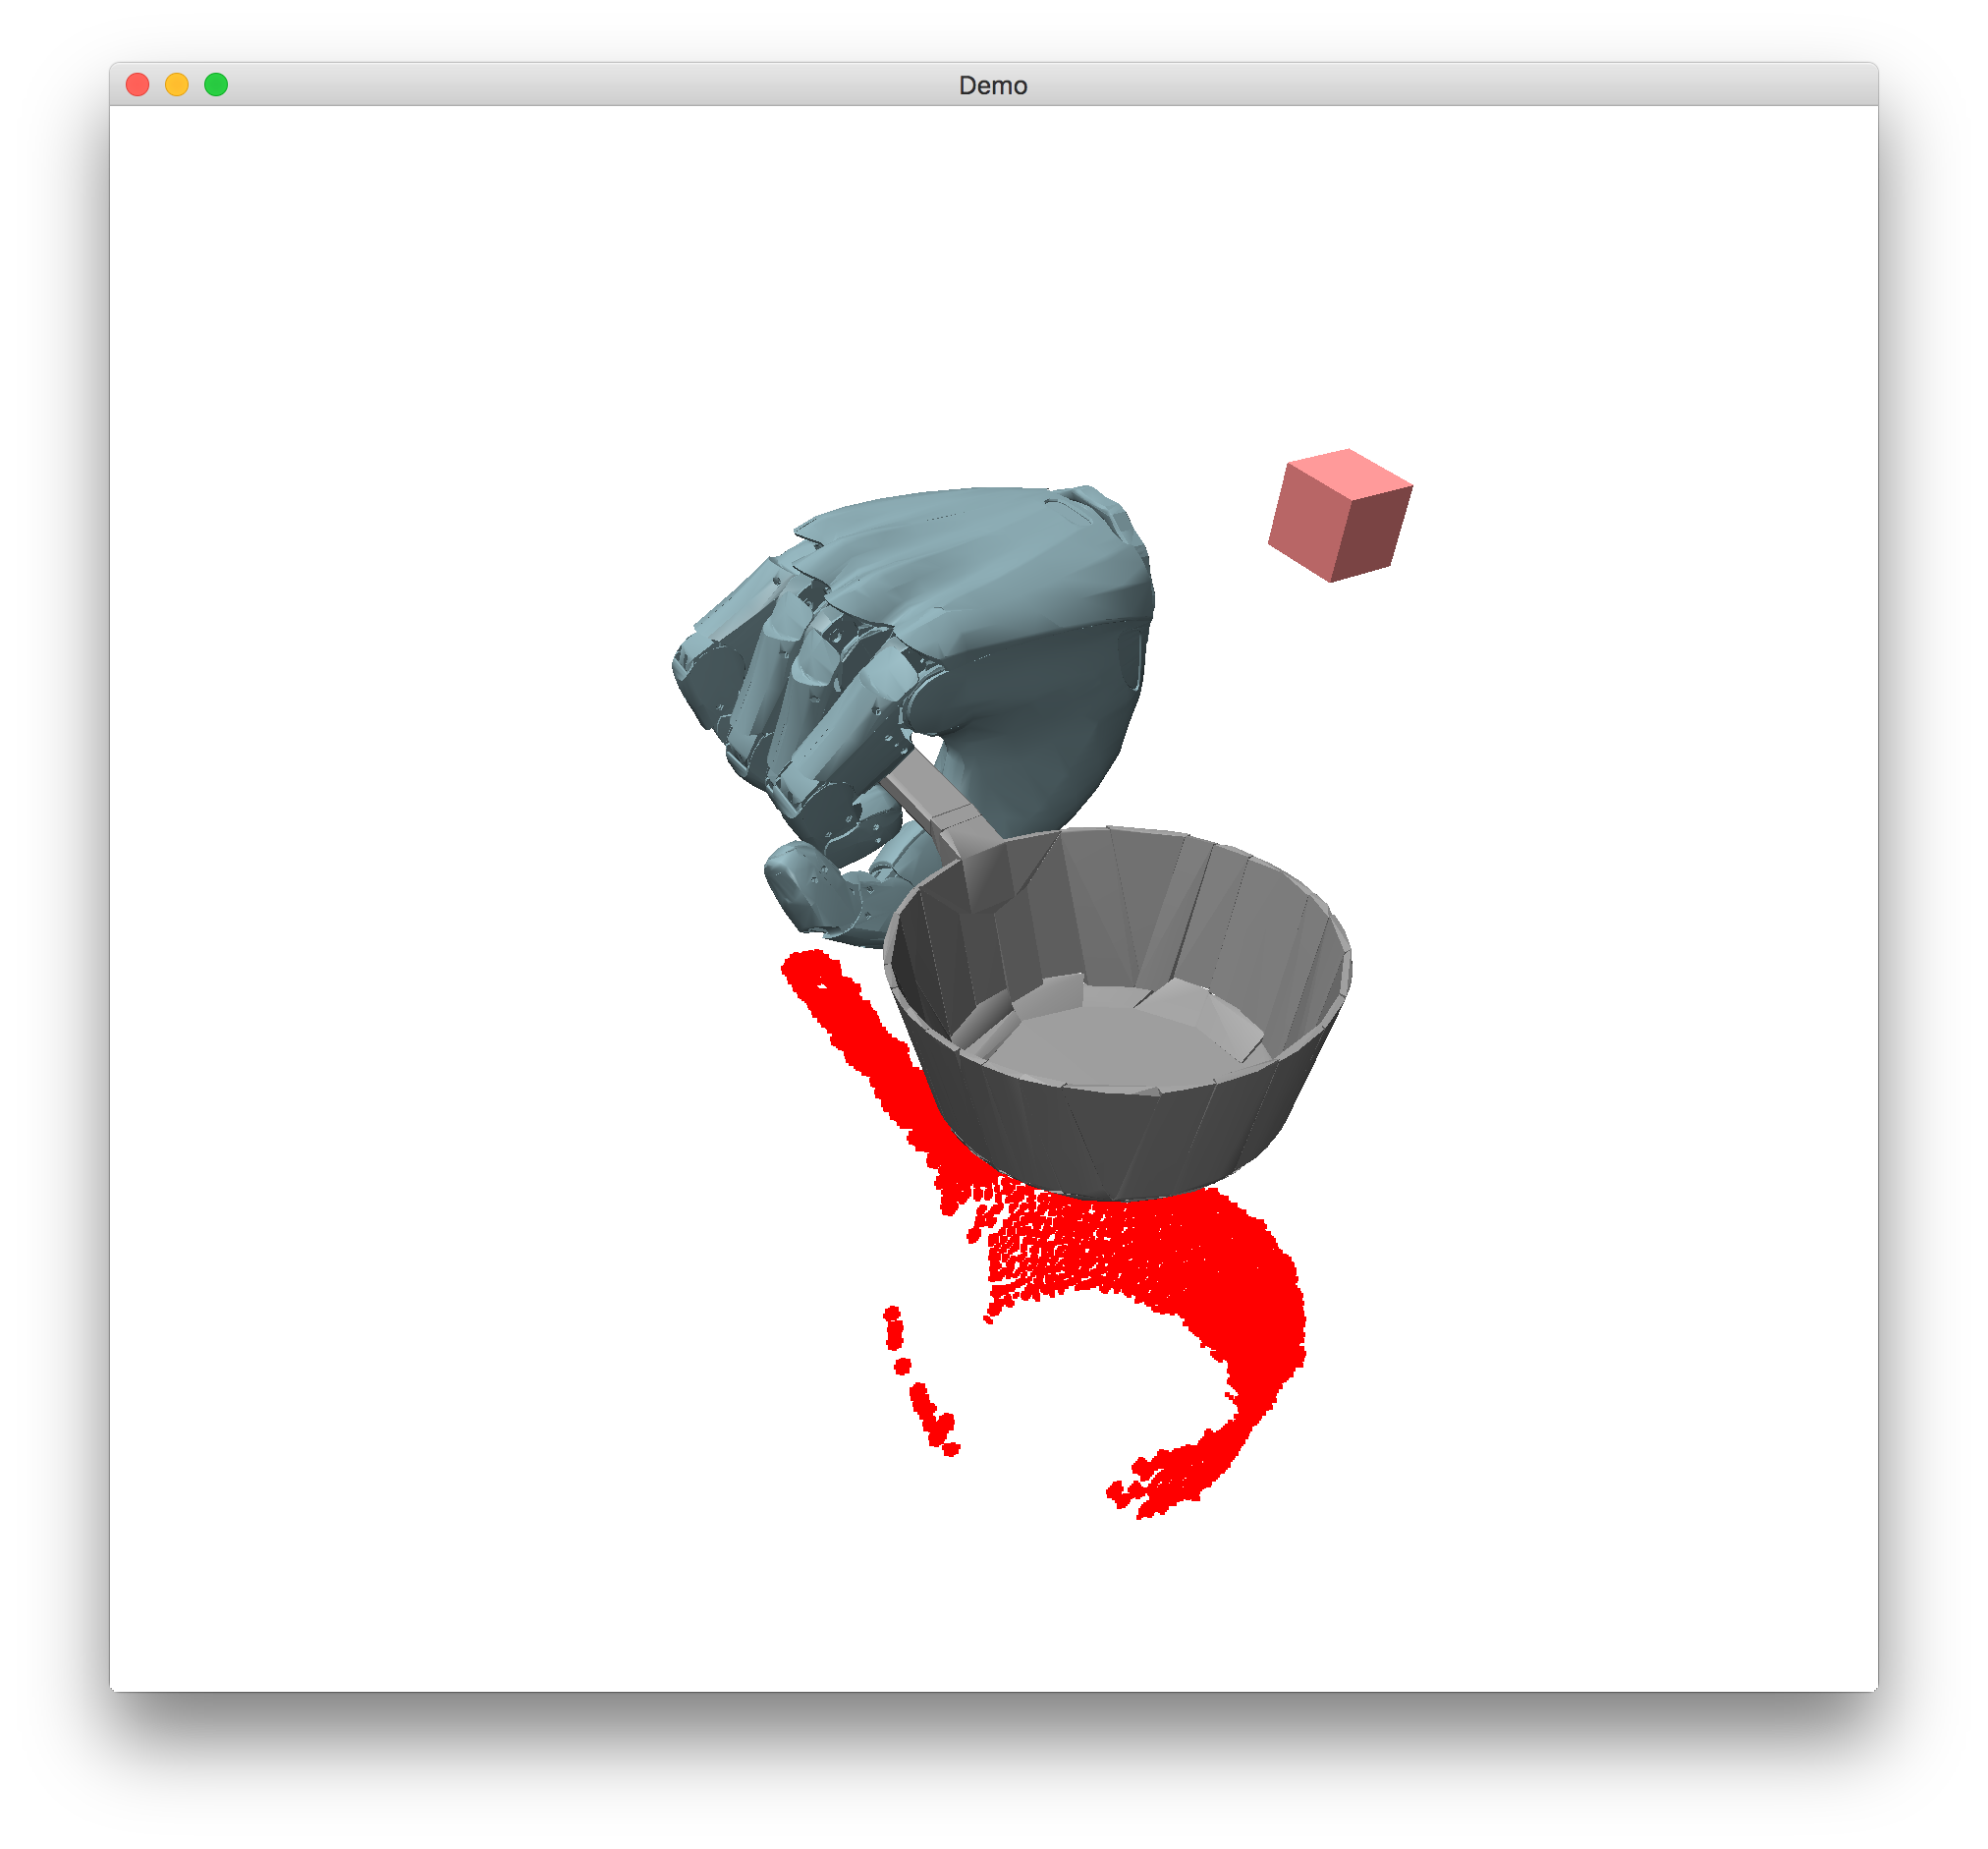
\includegraphics[width=0.24\textwidth]{images/Pan4_LFHW}
\caption{Creating a data set for robust evaluation. (Top row) The same pinch grasp, executed on the same object, with varying friction and mass parameters. (Bottom row) A more robust power grasp, executed on the same object, with the same variation in friction and mass. \label{fig:evaluative-training}}
\end{figure}

Using this method, we generated a data set (DS1) of 1.12 million simulated grasps using GM1 as the generative model and a data set of 1.136 million additional grasps (DS2) using GM2. Each grasp can be replayed in Mujoco and the set can be decomposed for train and test purposes as required. We give details of the statistics in Table including the way that we break down the data-set into training, validation and test subsets. The ratio of successful grasps in the dataset is less than 50\% for GM1, and is more than 50\% for GM2. In order to have a balanced training set, the number of successful and unsuccessful grasps have been equalised by under-sampling the failure cases in GM1 and over-sampling the failure cases for GM1. No balancing was performed for GM1/2 validation and test sets.
\begin{table*}[t]
\centering
\caption{Statistics of the simulated data sets.}
\label{tab:data}
\begin{tabular}{|l|l|l|l|l|l|l|l|l|l|l|} \hline
Data set & Generative &  Subset & \# Scenes & Top-grasp & Top-grasp & Top grasp & Total & Total  & Total  & Total \\ 
              & Model         &              &                   &  \# succs  & \# fails       & \% succs  & grasps   & \# succs      & \# fails  & \% succs  \\ \hline
 DS1-Tr & GM1 & Train & 17714 & 10100 & 7614 & 57.0\% & 959,882 & 479,941 & 479,941 & 50.0\% \\ \hline
 DS1-V  & GM1 & Validate & 1042 & 613 & 429 & 58.8\% & 61,393 & 29,557 & 31,836 & 48.1\% \\ \hline
 DS1-Te & GM1& Test & 1539 & 1070 & 469 & 69.5\% & 99,521 & 48,084 & 51,437 & 48.3\% \\ \hline
 DS2-Tr  & GM2 & Train & 5377 & 3771 & 1606 & 70.1\% & 943,481 & 533,282 & 410,199 & 56.5\% \\ \hline
 DS2-V   & GM2 & Validate & 544 & 378 & 166 & 69.4\% & 68,586 & 39,559 & 29,027 & 57.7\% \\ \hline
 DS2-Te  & GM2 & Test & 988 & 781 & 207 & 79.0\% & 124,137 & 73,836 & 50,301 & 59.5\% \\ \hline
\end{tabular}
\end{table*}

\section{Analysis in Simulation Data}
\label{section:simulationAnalysis}
This section presents a simulation analysis of the various architectures based on the two data sets. 
We assess each variant in two different ways. First, for any method with an evaluative model we  measure the prediction accuracy of the EM. We compare the actual outcomes in a test set with the EM's prediction as to whether it is more likely to succeed or fail (output set at a threshold of 0.5). This gives us a confusion matrix from which we can calculated sensitivity, specificity and F1 score. Second, since a robot can only execute one grasp, we can measure the proportion of successful top-ranked grasps for any method. In each analysis the test set effectively replaces the Generative Model as it contains, for any scene, a complete list of grasps. Thus TS1 contains grasps proposed by GM1 and TS2 contains grasps proposed by GM2. This allows us to simulate the effect of different generative models on performance. 

We performed both analyses and the results are given in Table~\ref{table:Results-sim}. When assessing pure GM architectures, we can only measure the top ranked grasp success, since the GMs give a grasp likelihood according to the generative model not a probability of success. 

The main findings are as follows. First, of the pure generative models GM2 outperforms GM1, with top ranked grasp successes of 79.05\% and 69.53\% respectively. Second, the GEA architectures all outperform both pure GM architectures, starting at 87.85\% of grasps succeeding (V3 based on proposals from GM1 and evaluation by EM3 trained on TS1). Third, the increase in training set size (adding GM2 to GM1) yields a further improvement. We can best measure this by considering the residual number of top grasps that fail as a percentage of the baseline (GM1). On this measure adding the additional data (variants V6-V9) improves performance (over variants V3-V5) by an average of 3\%. 

All the above results use GM1 as the generative model. We can measure the benefit of substituting this by GM2. This yields a further reduction in residual failures over GM1 under the same training conditions (training with DS1-Tr and DS2-Tr) of 3.5\%. 

In summary, simulation results provide evidence that: pure GM2 outperforms GM1; adding training data improves results; and using GM2 as the generative model in the generative-evaluative architecture improves results. 

%Recall that the generative-evaluative architecture (GEA) comprises both the generative model (GM) and the evaluative model (EM). 
%We can evaluate aspects of these separately. After training, the EM was used to predict grasp outcomes in the test set. This comprised 1,241 scenes with 76,213 grasps. Of these, 40,243 succeeded and 35,970 failed. Our analysis is given in Table~\ref{fig:predictions}. The sensitivity is 0.84 and the specificity 0.71. The F1-score is 0.802.
%\begin{table}[b]
%\centering
%\caption{Confusion matrix for prediction on simulated data.}
%\label{fig:predictions}
%\begin{tabular}{|c|c|c|c|c|c|}
%\hline
% & & \multicolumn{4}{c|}{Prediction} \\ \cline{3-6}
%      & & \multicolumn{2}{c|}{\#} & \multicolumn{2}{c|}{\%} \\ \cline{3-6}
%  &  & Succ         & Fail         & Succ         & Fail         \\ \hline
%\multirow{ 2}{*}{Ground Truth} \newline & Succ & 33890      & 6353       & 84\%     & 16\%       \\ \cline{2-6}
% &Fail & 10339      &  25631    & 29\%     &  71\%   \\ \hline
%\end{tabular}
%\end{table}
% In this context, precision is the fraction of correctly labeled grasps among those predicted to be of a certain class (success or failure). Recall stands for the fraction of relevant grasps that have been identified correctly among all grasps that belong to that class. The results show a high recall rate for successful grasps, and there are relatively more false positives than false negatives. This necessitates pairing our evaluative neural network with a generative model rather than a random grasp generator, which would likely result in very low quality grasps and consequently, more false positives. 

%To test our generative-evaluative learning architecture we compared the grasp it proposes to the grasp proposed by the generative learner alone. Since \citet{kopicki2015ijrr} showed a 77.7\% success rate with the original generative algorithm we generated a new test set that contained both more challenging objects and placed them in challenging poses. The difficulty single-view grasping with a depth camera depends greatly on the pose of the object relative to the camera. The set comprised 40 test objects (Figure~\ref{fig:real-objects}) and another six training objects. The training objects were used by the human to demonstrate ten example grasps (Figure~\ref{fig:generative-training}). The 40 test objects were used to generate 49 object-pose pairs. From the 40 objects, 35 belonged to object classes in the simulation dataset, while the remaining five do not. 

\begin{figure}[t]
  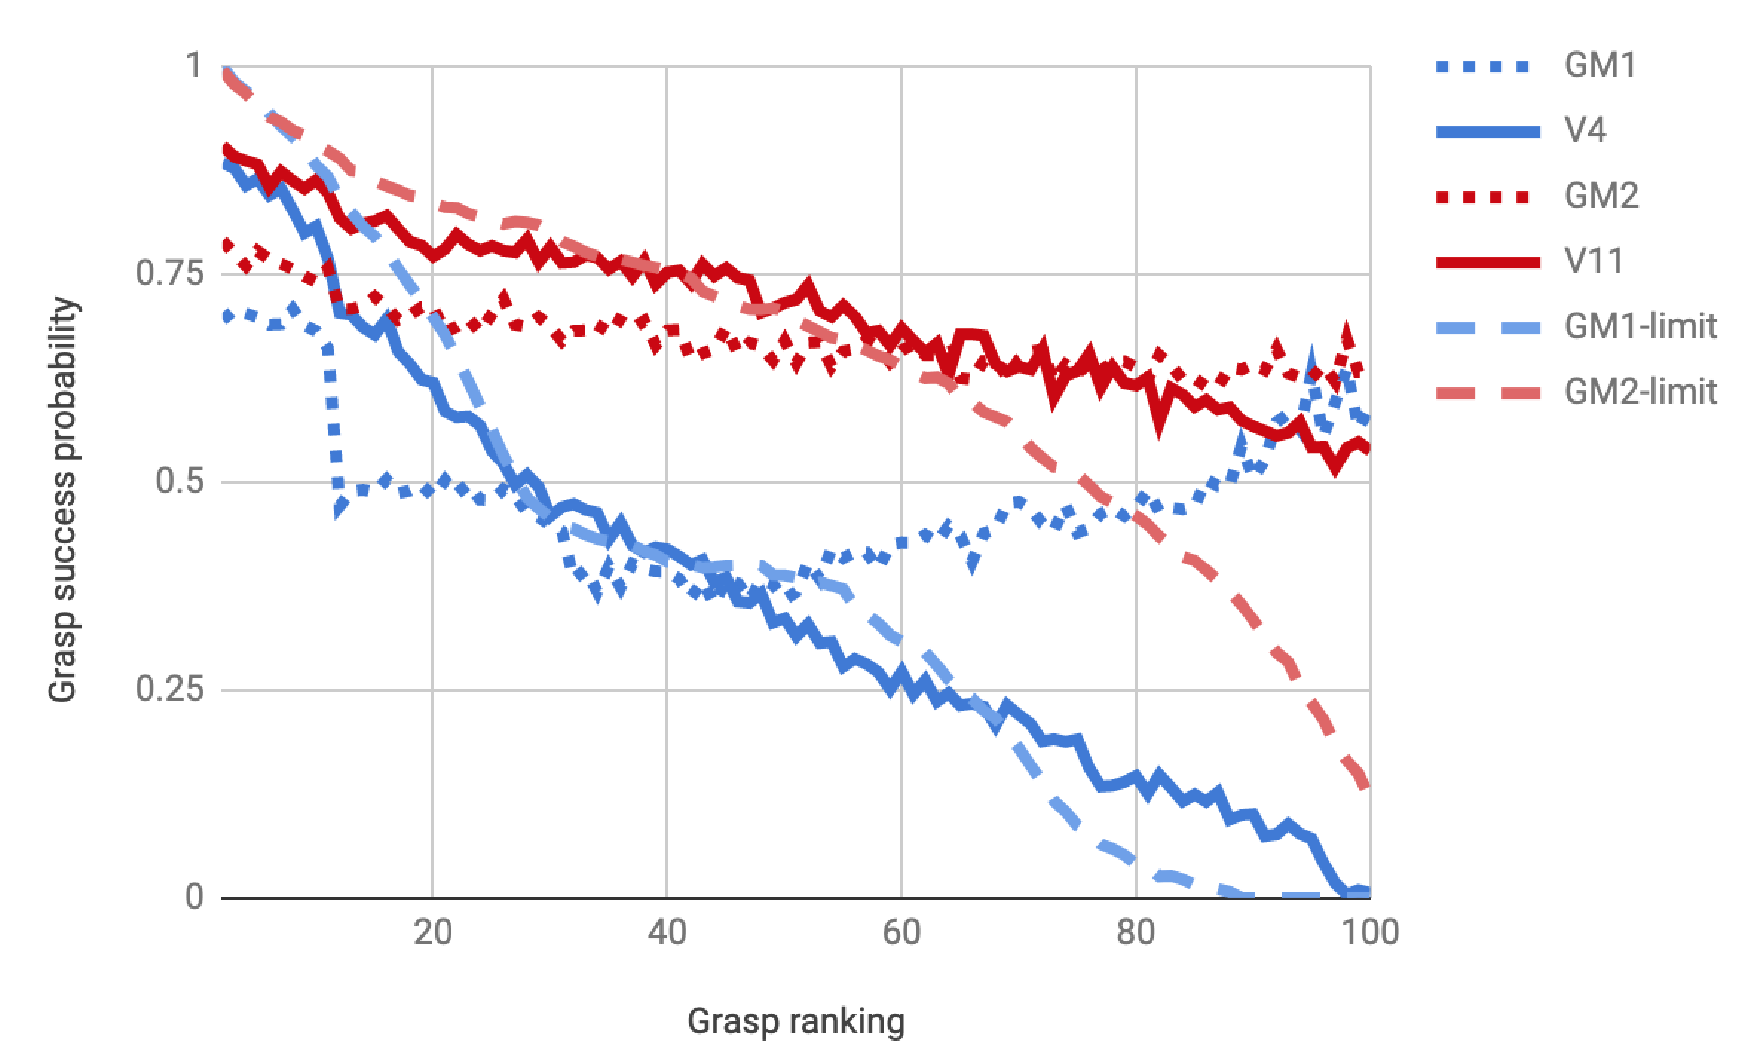
\includegraphics[width=\linewidth]{images/successvsranking.pdf}
  \caption{Grasp success probability (in simulation) vs. grasp ranking. GEA2 and GEA3 use GM1 and GM2 test data, respectively.}
  \label{fig:successvsranking}
\end{figure}

%We compared the EM and GM rankings (Figure~\ref{fig:successvsranking}). The x-axis shows the ranking. The y-axis shows the average actual success rate over all scenes (1,241 test, 7,311 training). When ranked by the EM, the grasp success probability falls nearly monotonically, as is desirable. On the other hand, the likelihood-based ranking of GM results in many good grasps being low-ranked. We also wish to know whether the grasps recommended by the EM and the GM have different grasp success rates. The success rates of the top-ranked grasps are 71.59\% (GM) and  84.2\% (EM).
So far we have considered only Generative-Evaluative architectures where the Evaluative Model merely ranks the grasp proposals. We also investigated using the EM to improve these grasps proposals. This essentially boils down to searching the grasp space driven by the EM as the objective function. This can be done either by gradient descent or using simulated annealing. The methods V12-17 use V11 as the objective function, hence V11 should be treated as the baseline. 

Lu et al. \cite{lu2017planning} proposed gradient ascent on the input grasp parameters to the EM with respect to the predicted success probability. They initialised with a heuristic grasp. We initialise with the best grasp proposed by the GEA. We experimented with three variants of the gradient ascent based tuning:
\begin{itemize}
\item GD1: Moves the entire trajectory at once in the world coordinate space, as directed by the average gradient on the trajectory's all 10 waypoints.
\item GD2: Tunes each finger joint individually. Each waypoint is treated independently.
\item GD3: Performs GD1 and GD2 simulatenously.
\end{itemize}

We ran the optimisation for 50 iterations, using a learning rate of 0.001 for position inputs and 0.01 for finger joints (We used different learning rates since the parameters are in different scales, GD1 in meters and GD2 in radians). Although predicted success rate rises, the success rate in simulation declines in all trials. We observed that the position changes have a more significant negative impact on the grasp success rate, when compared to finger joint movements. The results suggest that optimising dexterous grasps by the EM is non-trivial, perhaps because of the high-dimensionality of the grasp space. We speculate that initialising with a random grasp would be even worse.

Additionally, we implemented three variants of simulated annealing based optimisation:
\begin{itemize}
\item SA1: Moves the entire trajectory at once in the world coordinate space, using a three-dimensional Gaussian noise vector, with $\mu=0$ and $\sigma=0.001$. 
\item SA2: Perturbs the finger joints along the entire trajectory. The pose of all joints in a finger with respect to a reference pose (fully open hand) is modified, which results in an "opening/closing the finger" effect. We observed that this is a more natural movement rather than modifying a finger's joints independently. The opening/closing ratio for each finger is determined by a noise vector that is drawn from a Gaussian distribution with $\mu=0$ and $\sigma=0.01$. 
\item SA3: Performs SA1 and SA2 simulatenously.
\end{itemize}

The simulated annealing procedure contains up to 5 iterations, with 20 random perturbations in each. We start with a temperature of 0.2 and decrease it exponentially to 0.005 by halving it after every batch. If the current solution does not improve after three iterations, the optimisation stops. We do not accept any perturbations that will result in a collision with the table. Similarly with gradient ascent, the performance of the optimised grasps are worse than the baseline (V11). The effect of moving the trajectory is more significant when compared to the finger joints. TODO: Interpret the results.

\begin{table*}[t]
\centering
\begin{tabular}{|l|l|l|l|l|l|l|l|l|l|l|}
\hline
Variant \# & \multicolumn{2}{|c|}{Selected grasp} &  Succ \% & Residual Fails & Test set / GM& \multicolumn{5}{|c|}{Prediction Performance} \\ \hline
 & Succs & Fails &  & as \% of V1 fails &  & TP & FP & TN & FN & Accuracy \\ \hline
V1 & 1070   & 469 & 69.53\% & 100\% & GM1 & - & - & - & - & - \\ \hline
V2 &  781   & 207 & 79.05\% & 68.7\% & GM2 & - & - & - & - & - \\ \hline
V3 & 1352 & 187 & 87.85\% & 39.9\% & GM1 & 37840 &	12226 & 39211 & 10244 & 77.42\% \\ \hline
V4 &  1361 & 178 & 88.43\% & 38.0\% & GM1 & 40234 &	14475 & 36962 & 7850 & 77.57\% \\ \hline

V5 & 1361 & 178 & 88.43\% & 38.0\%& GM1 & 39603 & 14122 &37315 & 8481	& 77.29\% \\ \hline

V6 & 1375 & 164 & 89.34\% & 35.0\% & GM1 & 37584 &	11514 & 39923 &10500	& 77.88\% \\ \hline
V7 & 1363 & 176 & 88.56\% & 37.5\% & GM1 & 39332 &	12020 & 39417 & 8752 & 79.13\% \\ \hline
V8 & 1378 & 161 & 89.54\% & 34.3\% & GM1 & 37832 &	11361 & 40076	& 10252 & 78.28\% \\ \hline
V9 & 887 & 101 & 89.78\% & 33.5\% & GM2 & 61866 &	11454& 38847& 11970 & 81.13\% \\ \hline
V10 & 893 & 95 & 90.38\% & 31.6\% & GM2 & 64309 &	12517 & 37784 & 9527 & 82.24\% \\ \hline
V11 & 894 & 94 & 90.49\% & 31.2\% & GM2 & 61611 & 9792 & 40509 & 12225 & 82.26\% \\ \hline
V12 & 1319 & 220 & 85.71\% & 47.0\% & GM1 & - & - & - & - & - \\ \hline
V13 & 1375 & 164 & 89.34\% & 35.0\% & GM1 & - & - & - & - & - \\ \hline
V14 & 1366 & 173 & 88.76\% & 37.0\% & GM1 & - & - & - & - & - \\ \hline
V15 & 1153 & 386 & 74.92\% & 82.0\% & GM1 & - & - & - & - & - \\ \hline
V16 & 1377 & 162 & 89.47\% & 35.0\% & GM1 & - & - & - & - & - \\ \hline
V17 & 1163 & 376 & 75.57\% & 80.0\% & GM1 & - & - & - & - & - \\ \hline
\end{tabular}
\caption{Simulation results for all variants tested.}
\label{table:Results-sim}
\end{table*}
%A pure generative model architecture (GM) and the generative-evaluative architecture (GEA) were evaluated using a paired trials methodology. Each was presented with the same object-pose combinations. Each architecture generated a ranked list of grasps, and the highest ranked grasp was executed. The highest-ranked grasp based on the predicted success probability of the network is performed on each scene. A grasp was deemed successful if, when lifted for five seconds, the object then remained stable in the hand for a further five seconds before being automatically released. The success rate for GM was 57.1\% and for GEA it was 77.6\%. The successes and failures for each method were recorded and are summarised in Table~\ref{tab:robot-results}. A two-tailed McNemar test, for the difference between success rates for paired comparison data, was performed and the difference between the two algorithms has a $p$-value of 0.0442, and so is statistically significant. A selection of grasps where the two methods performed differently are shown in Figure~\ref{fig:successfail}.

% OLD TABLE
%\begin{table}
%\begin{center}
%\caption{Results of the real robot paired comparison trial.}
%\begin{tabular}{|c|c|c|c|}  \hline 
%          &                & \multicolumn{2}{ c |}{ GM} \\ \hline
%          &                & \# succs & \# fails  \\  \hline
 %GEA  & \# succs &  23 &  15  \\
 %         & \# fails    &  5   &   6   \\ \hline
%\end{tabular}
%\end{center}
%\label{tab:robot-results}
%\end{table}

%Training parameters for network. Training of example grasps for learning from demonstration. Creation of real test data set. Paired comparisons methodology with vanilla LFD algorithm (pose + object + camera view).
%
%The actual grasping tests have been performed on the real robot. 

\section{Real robot experiment}
\label{section:experiments}

\begin{figure}[t]
\begin{center}
  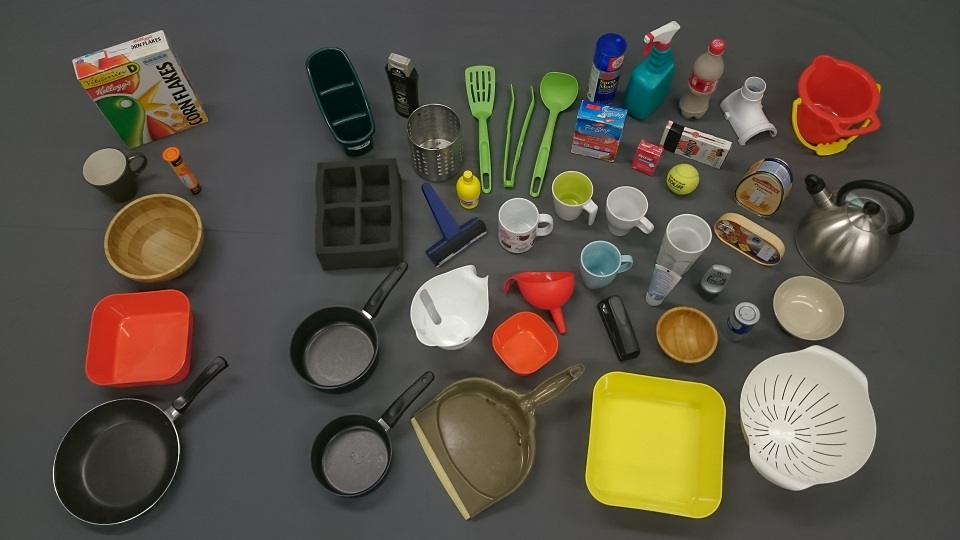
\includegraphics[width=0.7\linewidth]{images/objects.jpg}
  \end{center}
  \caption{The real objects. The training objects are on the left, testing objects are on the right.}
  \label{fig:real-objects}
\end{figure}

\begin{table}[b]
\small
\begin{center}
\caption{Performance on the real robot. \label{tab:robot-results}}
\begin{tabular}{|c|c|c|c|c|c|} \hline
Alg & \# succ & \% succ & Alg & \# succ & \% succ \\ \hline
V1  &  28 & 57.1\% & V4   & 37  & 75.5\% \\
V2  & 40 & 81.6\% & V11 & 43  & 87.8\% \\
\hline
\end{tabular}
\end{center}
\end{table}

\begin{figure}[t]
\begin{center}
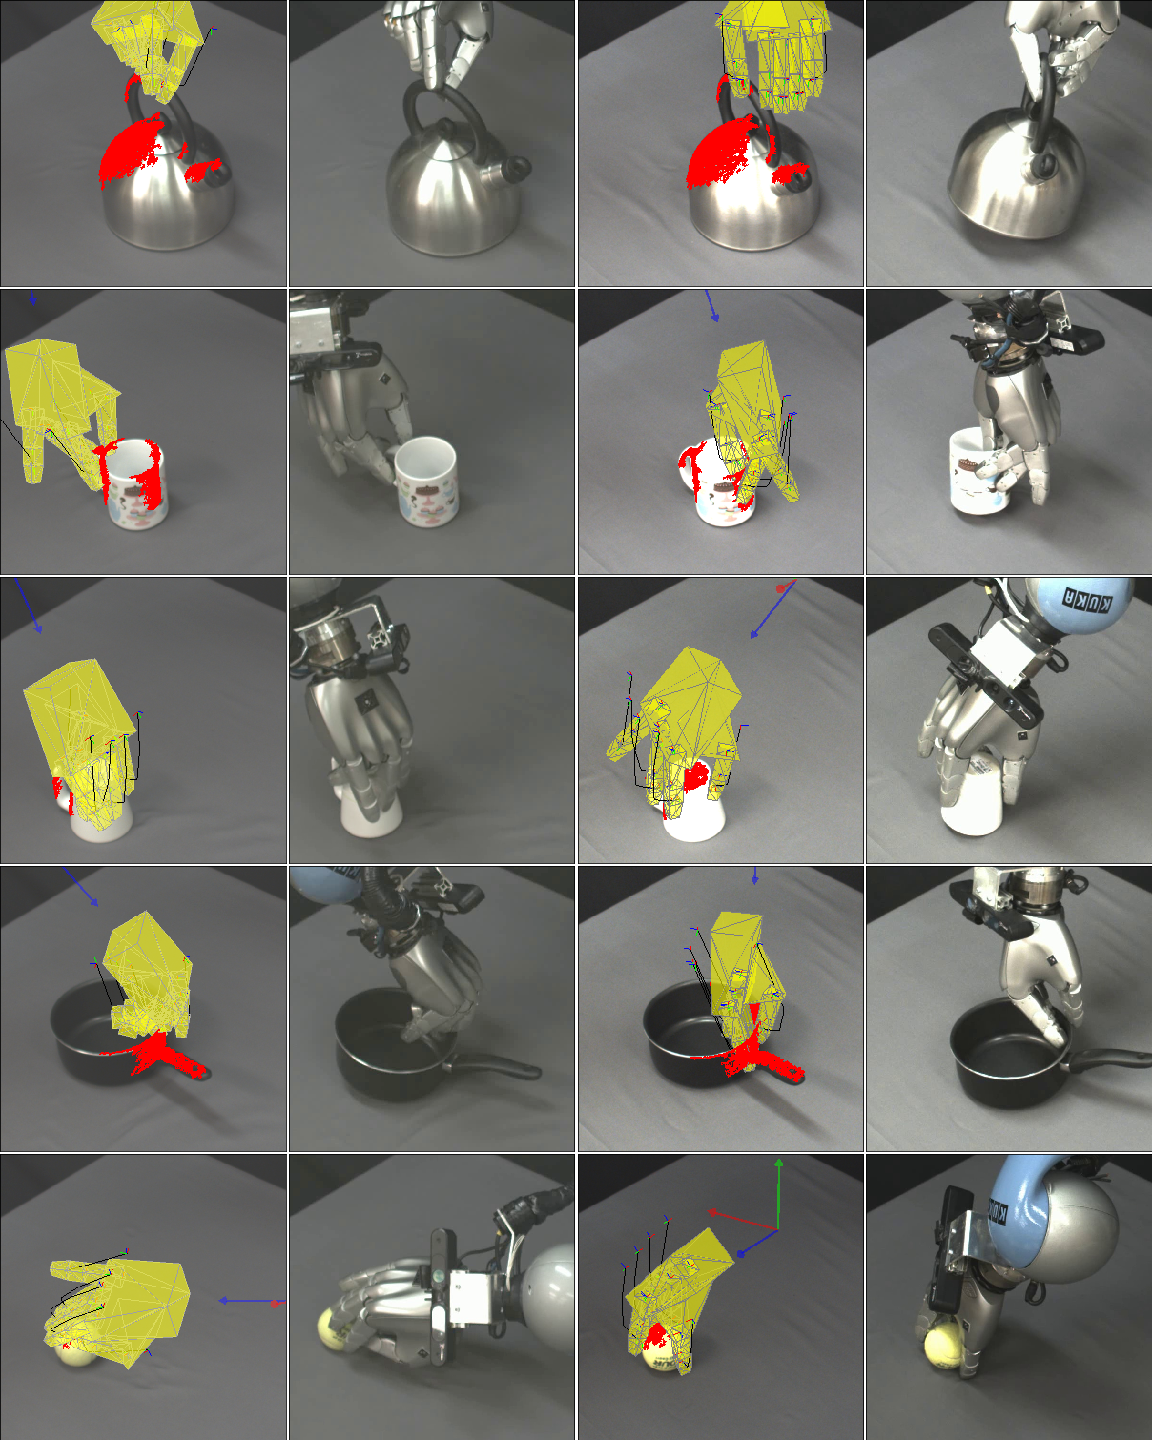
\includegraphics[width=0.5\columnwidth]{plots/A6fA10s_vertical.png}
\caption{V2 vs V11. This shows grasps from methods based on generative model GM2. The V2 grasps are shown in columns 1-2. The corresponding V11 grasps are shown in columns 3-4. These are the cases where V2 failed and V11 succeeded. \label{fig:v2fv11s}}
\end{center}
\end{figure}

\begin{figure}[t]
\begin{center}
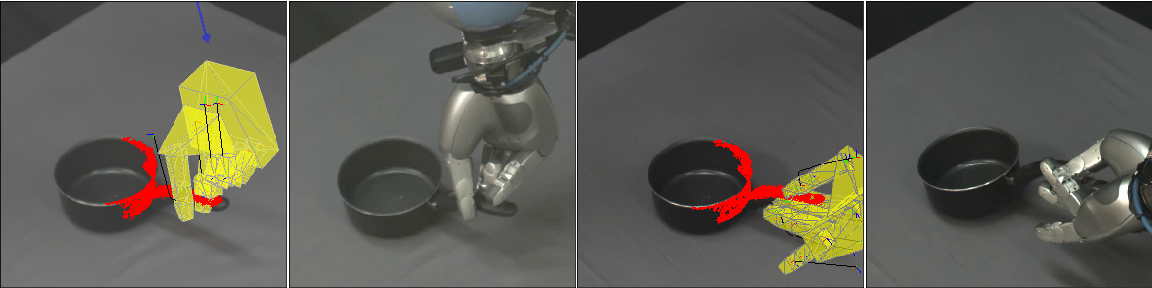
\includegraphics[width=0.5\columnwidth]{plots/A6fA10f_vertical.png}\\
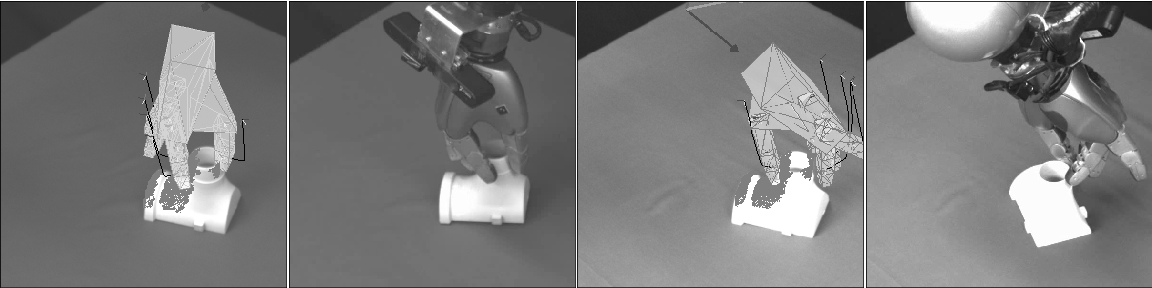
\includegraphics[width=0.5\columnwidth]{plots/A6sA10f_vertical.png}
\caption{V2 vs V11. This shows grasps from methods based on generative model GM2. The V2 grasps are shown in columns 1-2. The corresponding V11 grasps are shown in columns 3-4. The top row shows the case where both failed. The bottom row shows the case where V2 succeeded and V11 failed. \label{fig:v2fsv11f}}
\end{center}
\end{figure}


We compared four variants on the real robot: V1, V2, V4 and V11. V1 and V2 are the pure generative models. V4 is, in simulation, the equal best generative-evaluative method using GM1 as the generative model. It uses EM2 as the evaluative model. V11 is, in simulation, the best performing generative-evaluative method using GM2 as the generative model. This selection allows us to compare the best generative-evaluative methods with their counterpart pure generative models. 

We employed the same real objects as described in \cite{kopicki2019ijrr}. This used 40 novel test objects (Figure~\ref{fig:real-objects}). Object-pose combinations were chosen to reduce the typical surface recovery. Some objects were employed in several poses, yielding 49 object-pose pairs. From the 40 objects, 35 belonged to object classes in the simulation dataset, while the remaining five did not. 

Using this data-set, all algorithms were evaluated on the real-robot using a paired trials methodology. Each was presented with the same object-pose combinations. Each variant generated a ranked list of grasps, and the highest ranked grasp was executed. The highest-ranked grasp based on the predicted success probability of an evaluative network is performed on each scene. A grasp was deemed successful if, when lifted for five seconds, the object then remained stable in the hand for a further five seconds. 

The results are shown in Table~\ref{tab:robot-results}. In each case, the generative-evaluative variant outperforms the equivalent pure GM variant. So that V4 outperforms V1 by 75.5\% grasp success rate to 57.1\% and V11 outperforms V2 87.8\% to 81.6\%. The differences between V11:V1 and V2:V1 are highly statistically significant ($p<0.01$) using McNemar's test. Thus, we have strong support for our main hypothesis, which is that a Generative-Evaluative architecture outperforms a pure generative model. Six of the available grasp types were deployed (pinch support, pinch, pinchbottom, rimside, rim and power edge), showing that a variety of grasps is utilised.
%The success rate for GM1 was 57.1\% and for the top-performing method based on GM1, GEA.1, it was 77.6\% (Table~\ref{tab:robot-results}). The success rate of the second baseline, GM2, is 81.6\%, while GEA.3 shows outperforms it with a success rate of 87.8\%. A two-tailed McNemar test, for the difference between success rates for paired comparison data, was performed. The difference between the two algorithms has a $p$-value of 0.0442, and so is statistically significant. A selection of grasps where the two methods performed differently are shown in Figure~\ref{fig:successfail}.

% OLD TABLE
%\begin{table}
%\begin{center}
%\caption{Results of the real robot paired comparison trial.}
%\begin{tabular}{|c|c|c|c|}  \hline 
%          &                & \multicolumn{2}{ c |}{ GM} \\ \hline
%          &                & \# succs & \# fails  \\  \hline
 %GEA  & \# succs &  23 &  15  \\
 %         & \# fails    &  5   &   6   \\ \hline
%\end{tabular}
%\end{center}
%\label{tab:robot-results}
%\end{table}

%\begin{table}
%\begin{center}
%\caption{Results of the real robot paired comparison trial.}
%\label{my-label}
%\begin{tabular}{|cc|c|c|l}
%\cline{1-4}
%                                           &         & \multicolumn{2}{c|}{GM} &  \\ \cline{3-4}
%                                           &         & \# succs    & \# fails    &  \\ \cline{1-4}
%\multicolumn{1}{|c|}{\multirow{2}{*}{GEA}} & \# succs & 23         & 15         &  \\
%\multicolumn{1}{|c|}{}                     & \# fails & 5          & 6          &  \\ \cline{1-4}
%\end{tabular}
%\end{center}
%\label{tab:robot-results}
%\end{table}

\begin{figure*}
\begin{center}
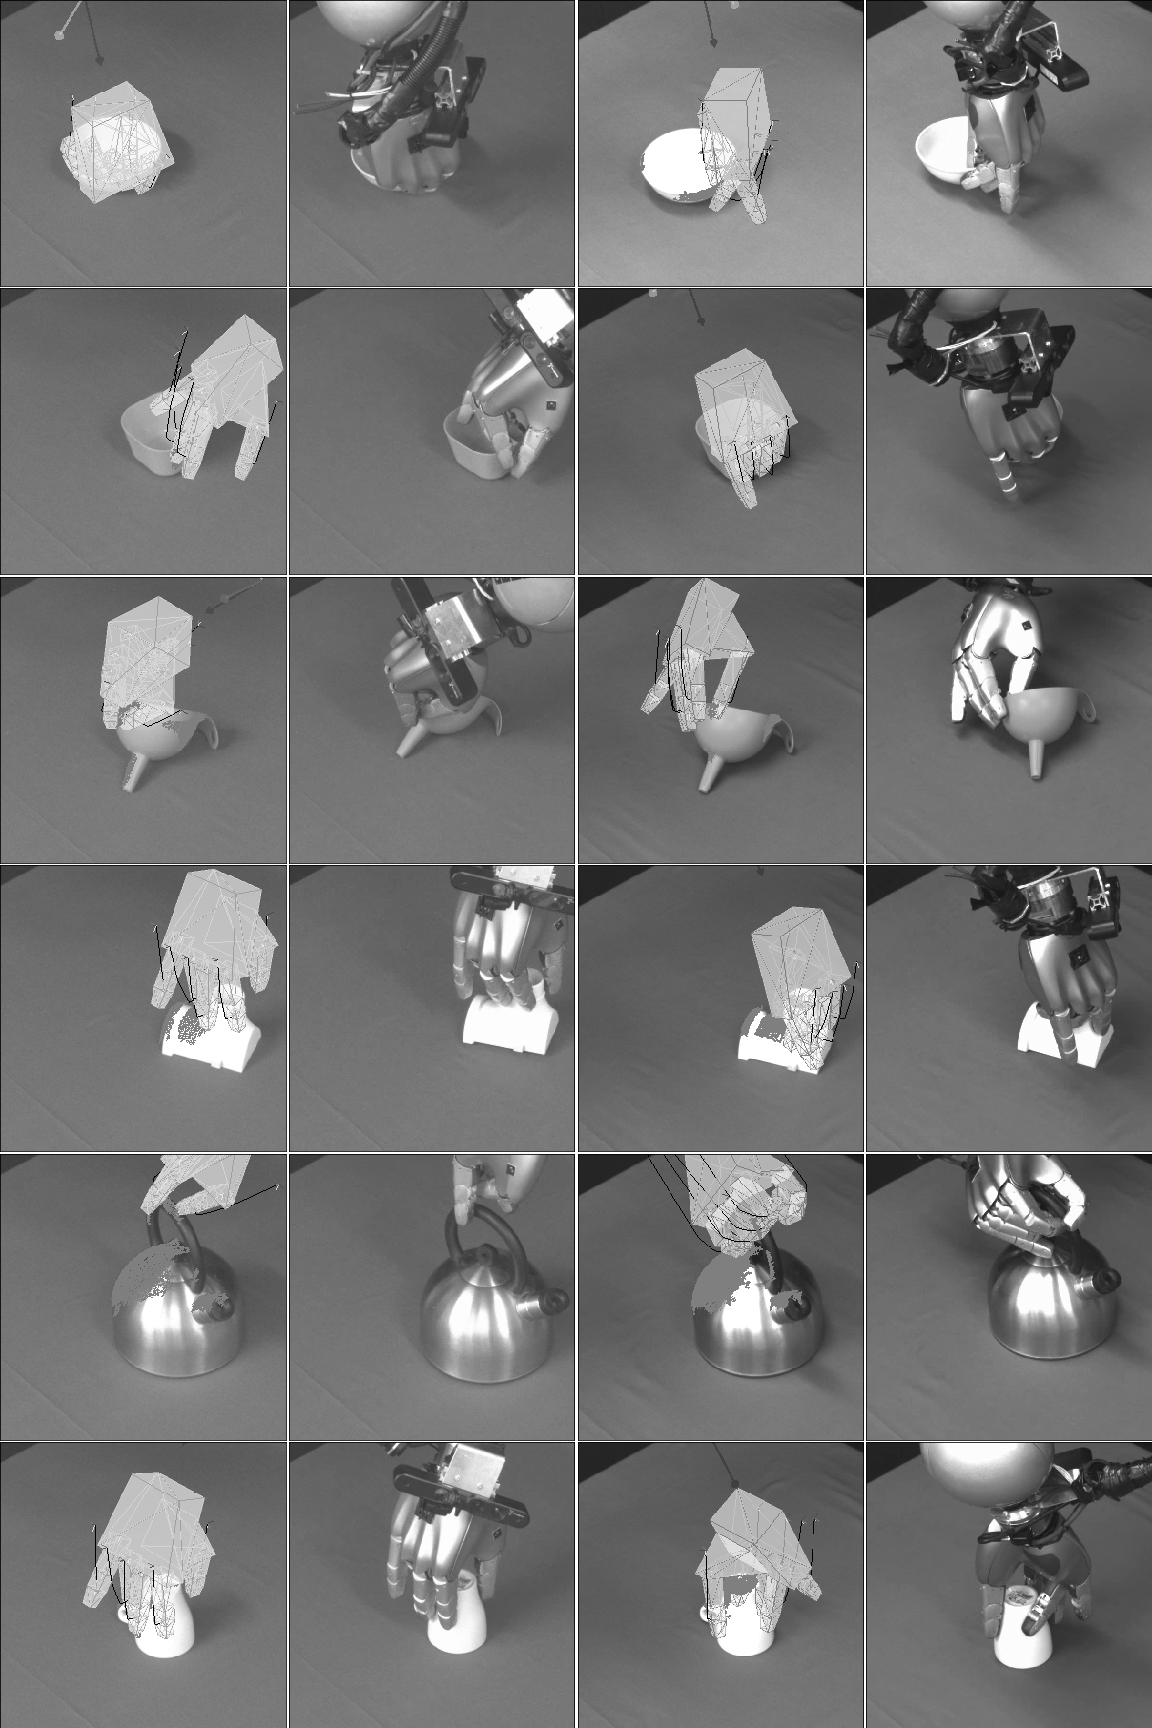
\includegraphics[width=0.48\textwidth]{plots/A2fA9s_1_vertical.png}~
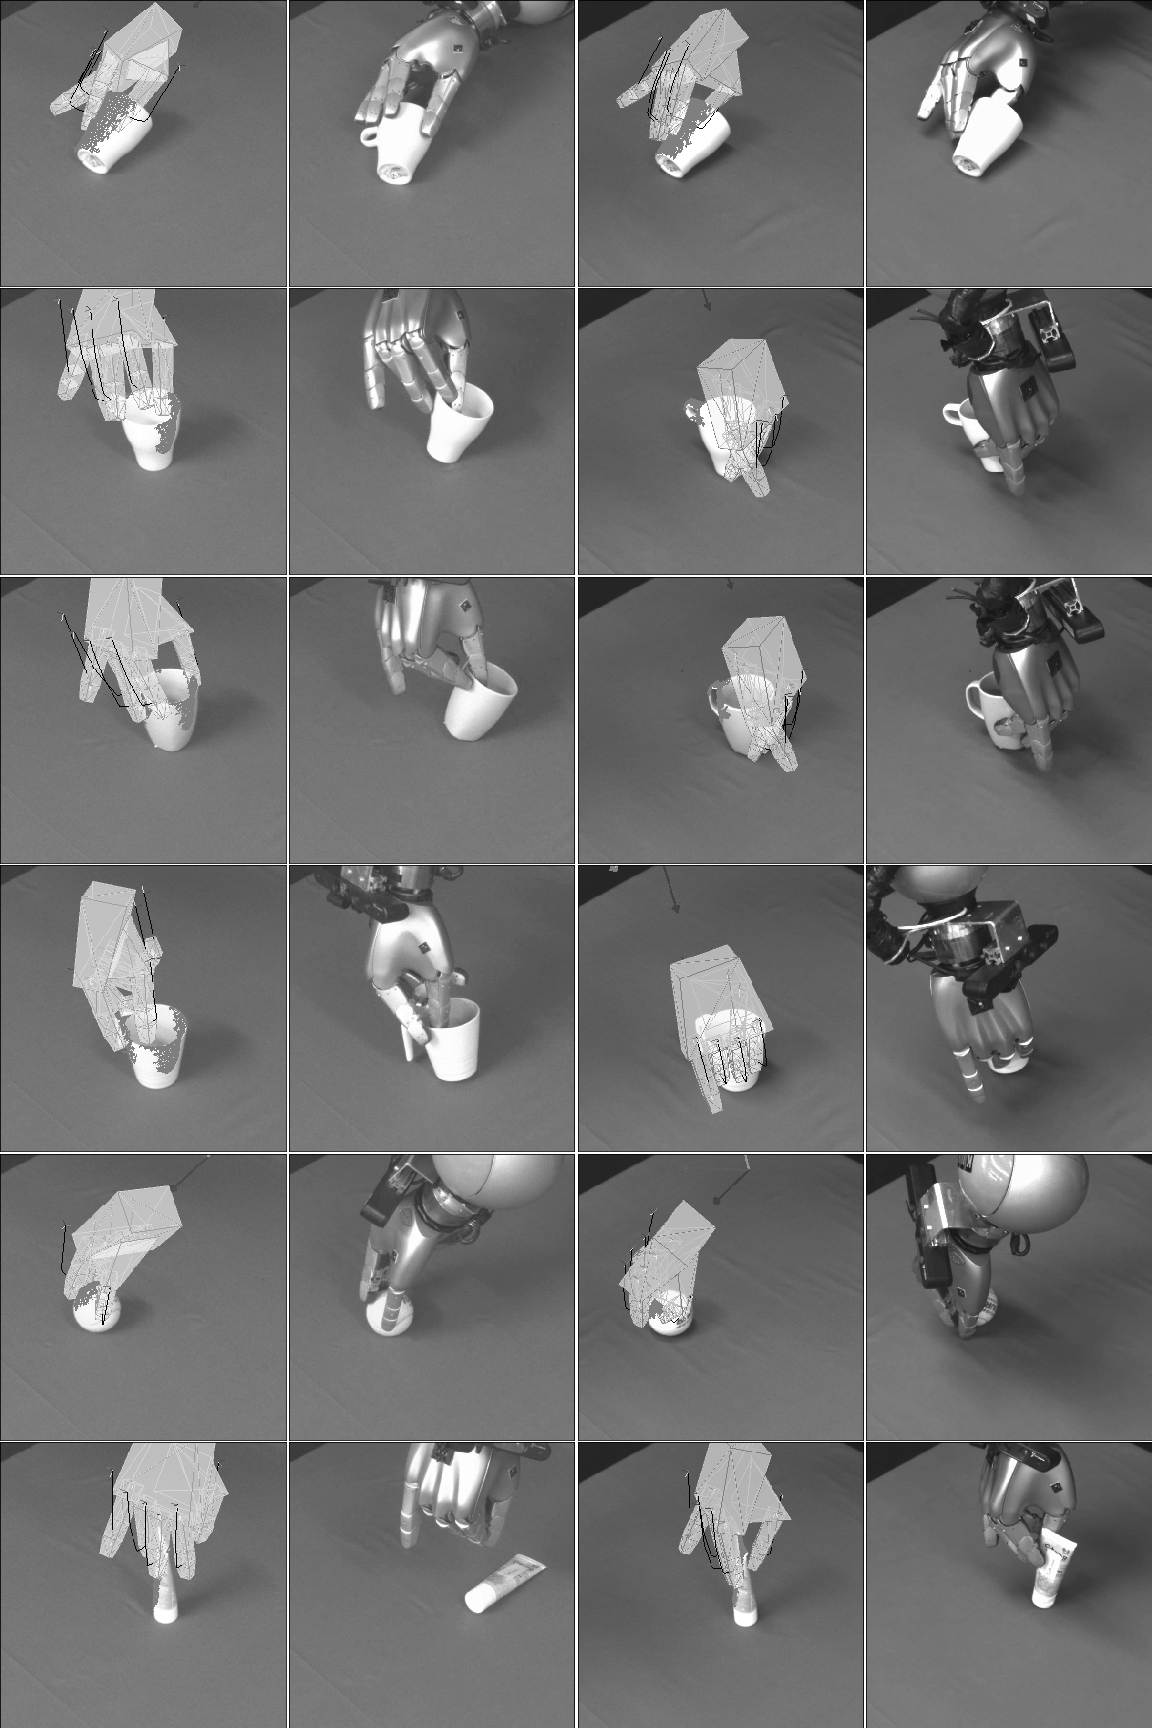
\includegraphics[width=0.48\textwidth]{plots/A2fA9s_2_vertical.png}
\caption{V1 vs V4. This shows grasps from methods based on generative model GM1. The V1 grasps are shown in columns 1-2 and 5-6. The corresponding V4 grasps are in columns 3-4 and 7-8. These are the cases where V1 failed and V4 succeeded.\label{fig:v1fv4s}}
\end{center}
\end{figure*}


\begin{figure*}
\begin{center}
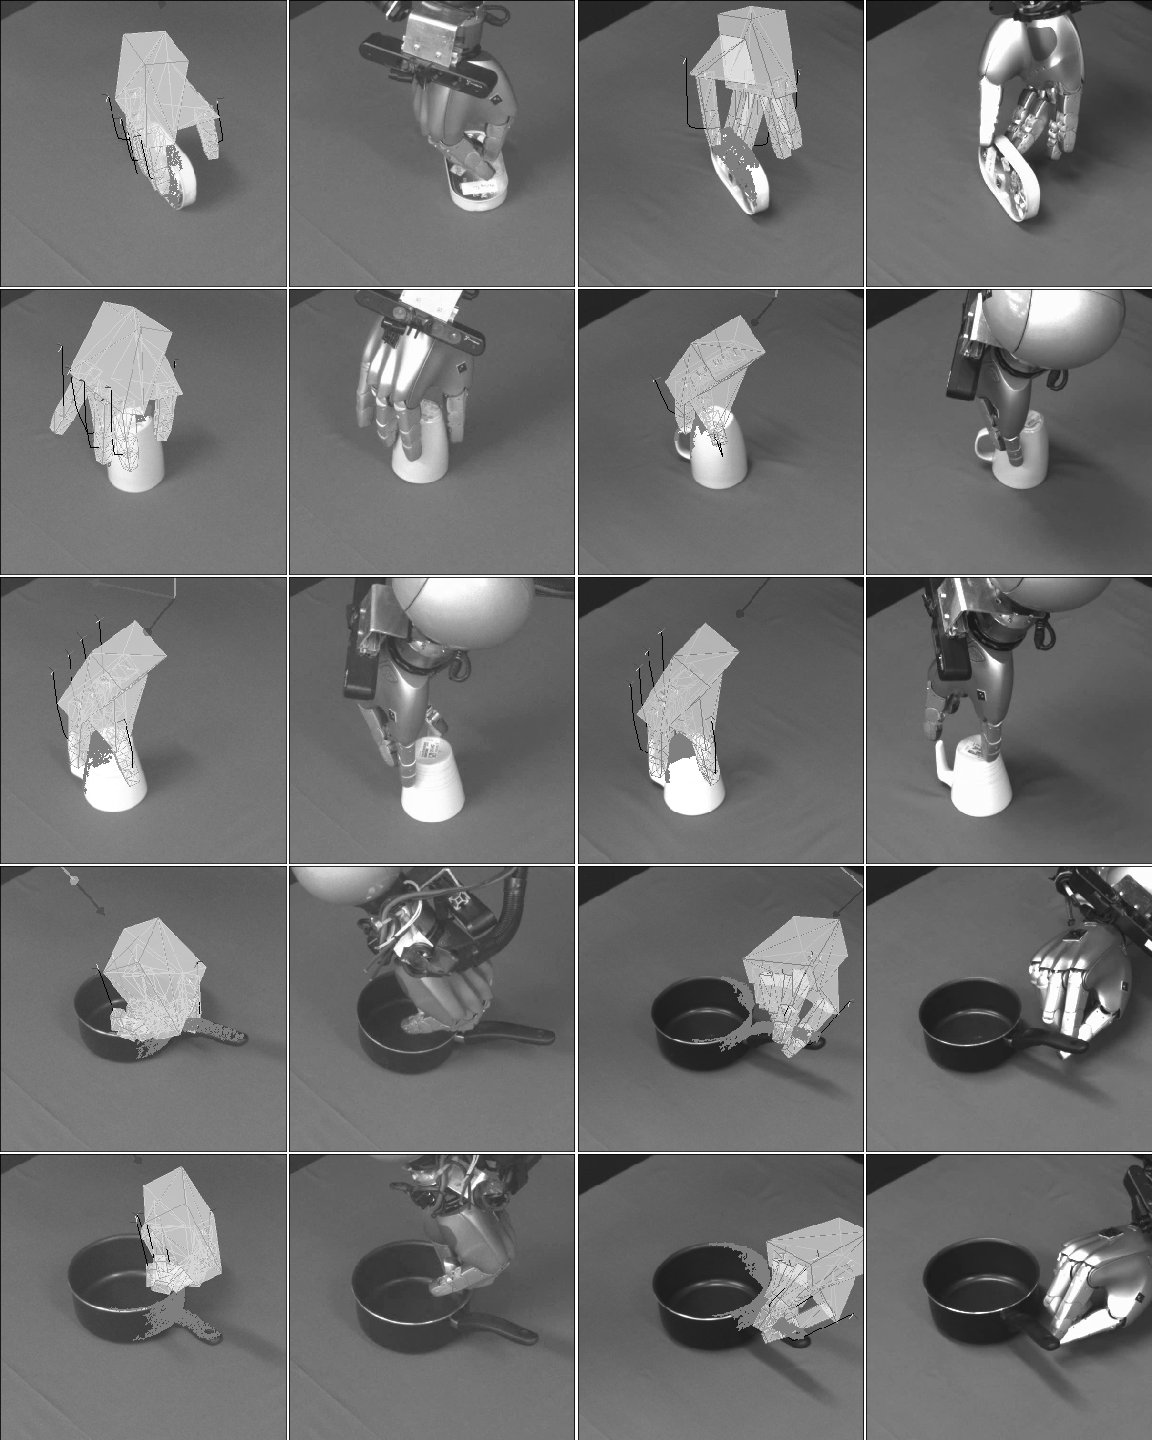
\includegraphics[width=0.48\textwidth]{plots/A2fA9f_vertical.png}~
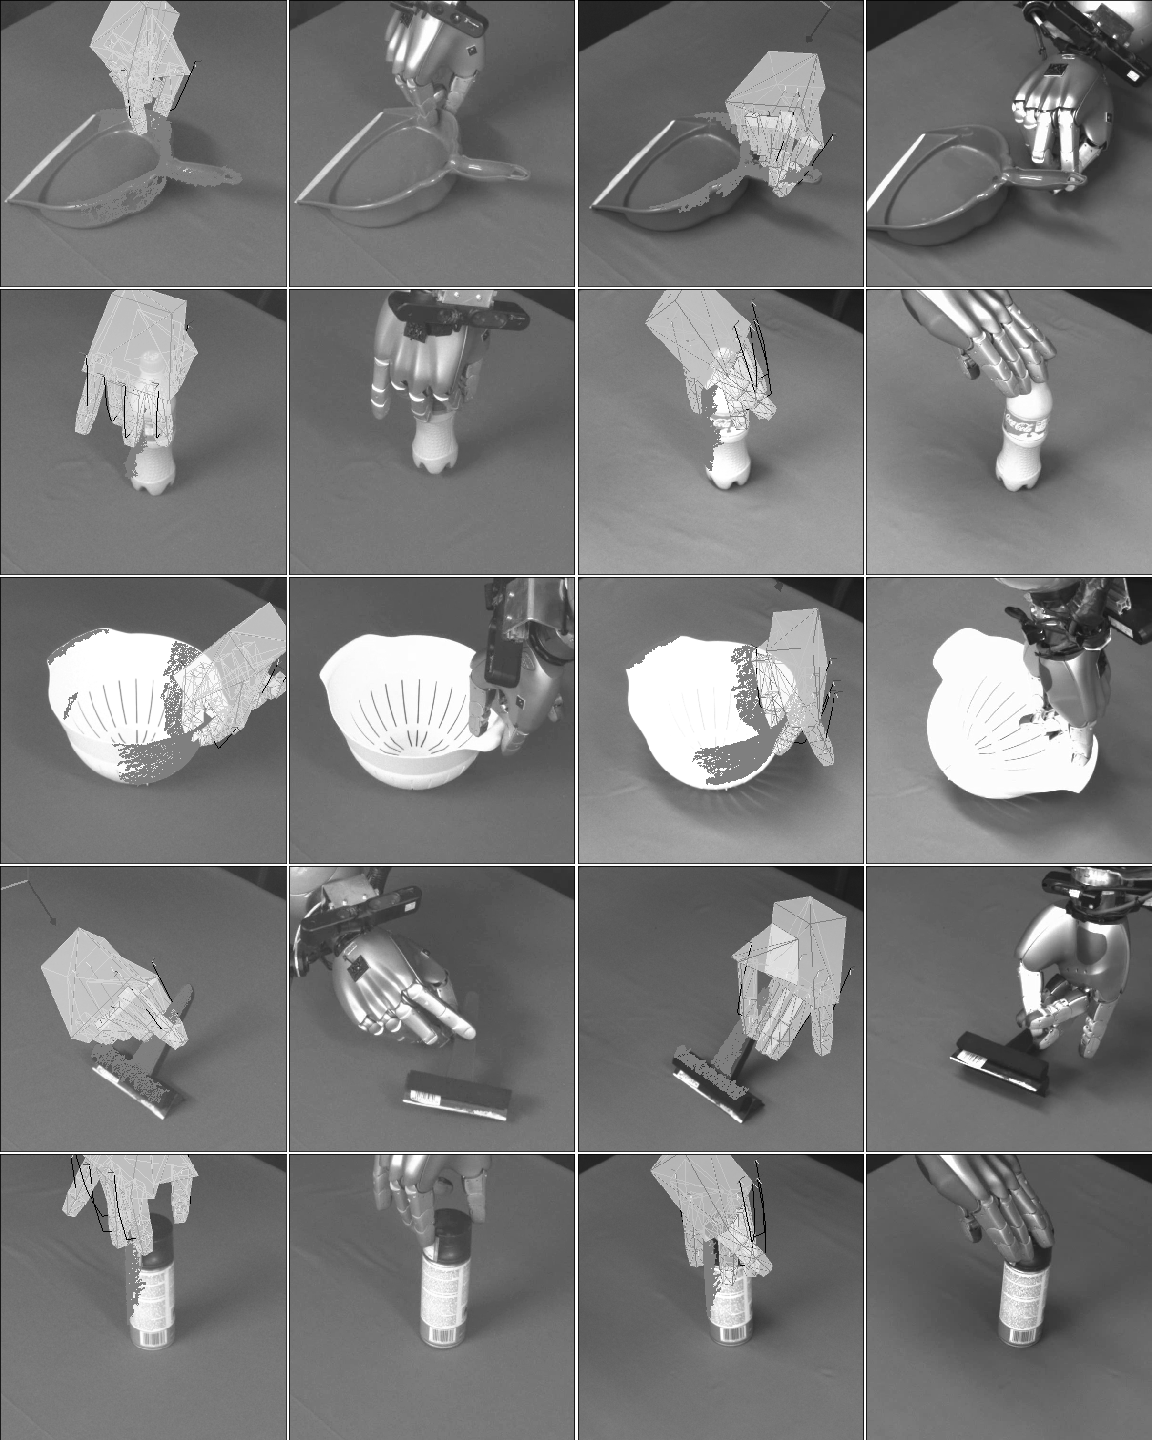
\includegraphics[width=0.48\textwidth]{plots/A2sA9f_vertical.png}
\caption{V1 vs V4. This shows grasps from methods based on generative model GM1. The V1 grasps are shown in columns 1-2 and 5-6. The corresponding V4 grasps are shown in columns 3-4 and 7-8. The left panel shows the cases where both V1 and V4 failed, while the right one shows the cases where V1 succeeded and V4 failed. \label{fig:v1fsv4f}}
\end{center}
\end{figure*}

%\begin{figure*}
%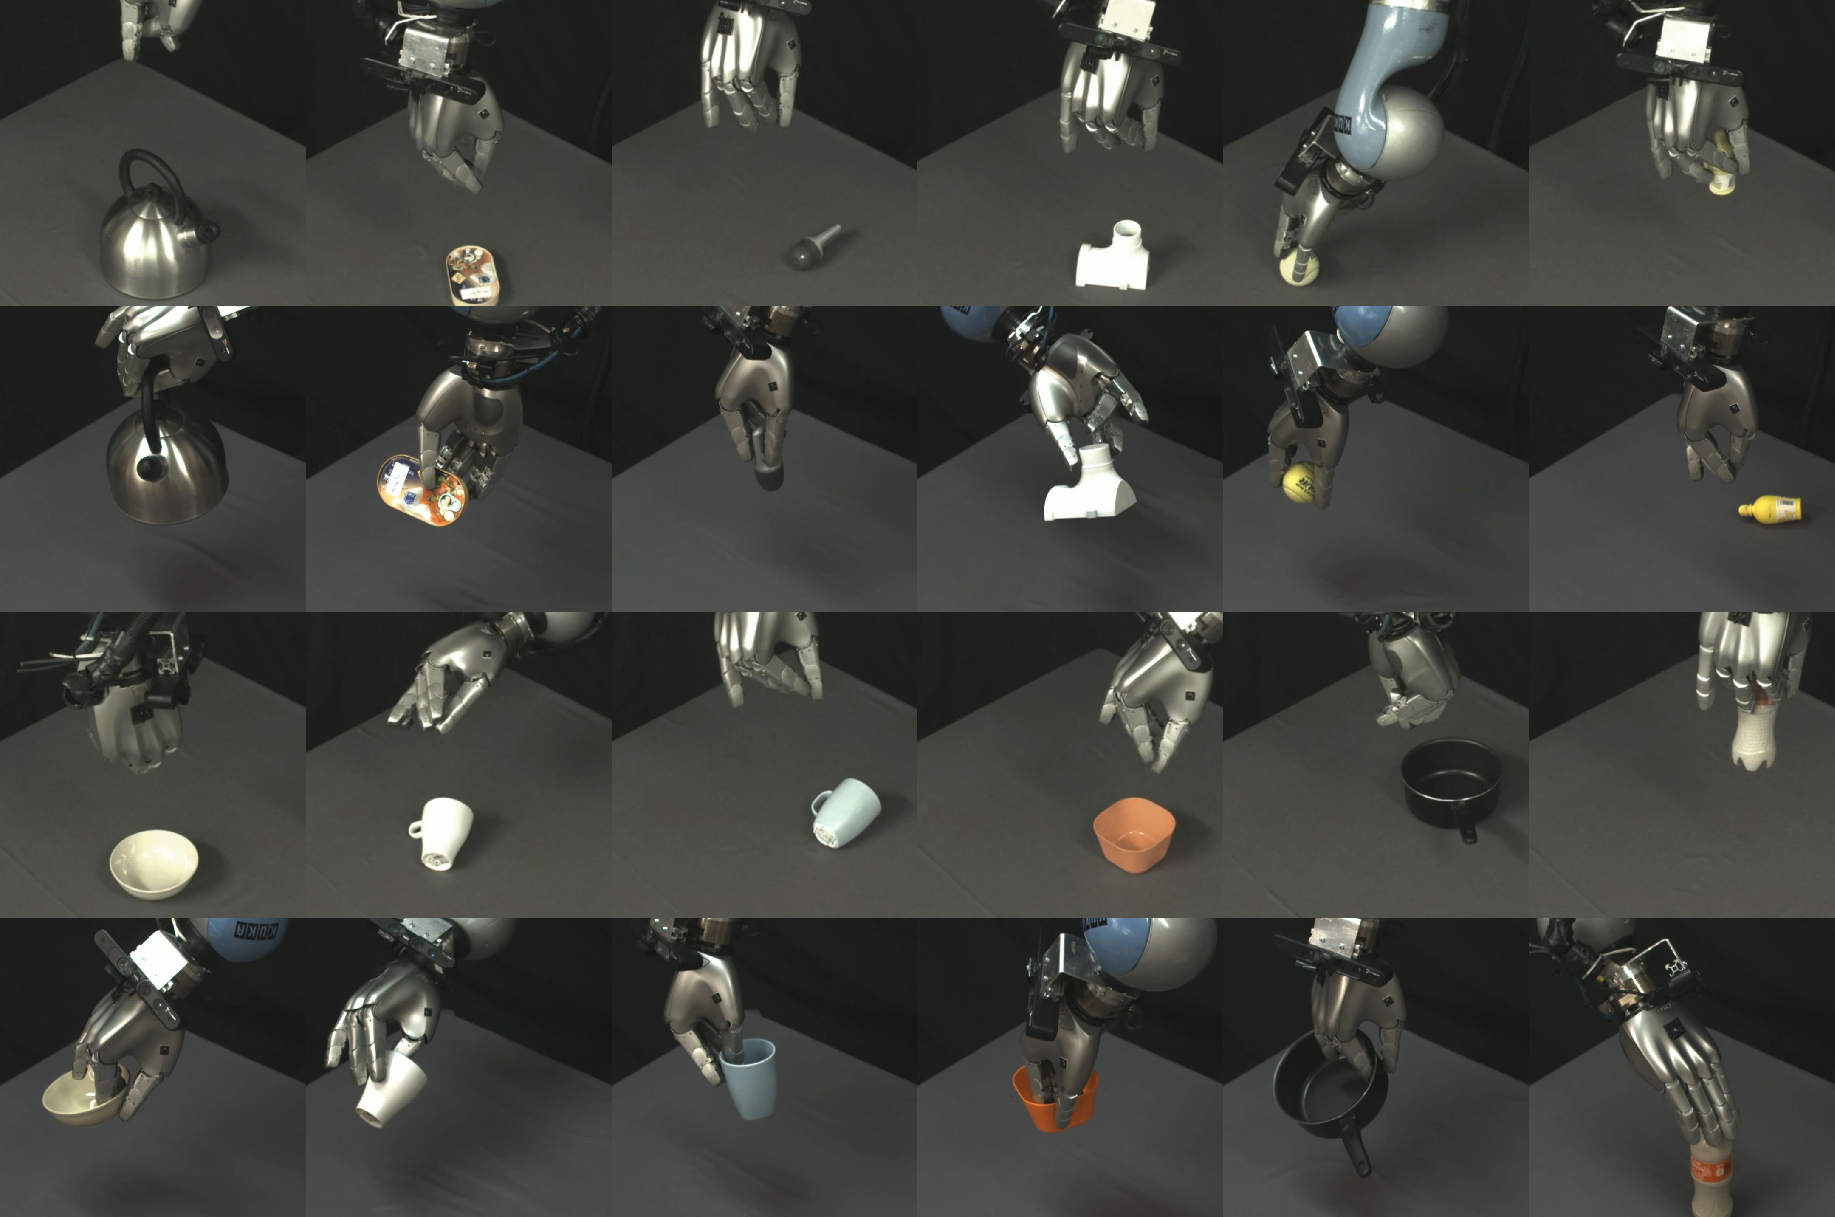
\includegraphics[width=\textwidth]{images/successfailure.pdf}
%\caption{Examples of grasps generated by the generative model (GM, $1^{st}$ and $3^{rd}$ row) and the generative-evaluative model (GEA, $2^{nd}$ and $4^{th}$ row) on paired trials. The first five columns show some of the 15 cases where the GEA model succeeds but GM fails. The far right-hand column shows 2 of the 5 converse cases. \label{fig:successfail}}
%\end{figure*}

%Training parameters for network. Training of example grasps for learning from demonstration. Creation of real test data set. Paired comparisons methodology with vanilla LFD algorithm (pose + object + camera view).
%
%The actual grasping tests have been performed on the real robot. 

\section{Conclusion} 
\label{sec:conclusion}

The challenge for dexterous grasping of novel objects from a single view is to quickly generate feasible grasps, and to have some measure of confidence that they will succeed. The way we have addressed this is to use two learned models: one generative, one evaluative. First, we learn a generative model using a highly data efficient method for learning from demonstration. This learns a good prior over feasible grasps in a way that can be transferred to novel objects, from just ten exemplars. This generative model is then used to generate grasps for novel objects, tested in simulation, the results of which are used to train an evaluative model with a data intensive learning algorithm. By testing simulated grasps across unobservable parameters such as friction and mass we can create an evaluative model that is robust to unobservable variation. We showed experimentally that our generative-evalutive architecture  improves the grasp success rate on real novel objects from substantially, and this difference is statistically significant at 0.05. 

%\section*{Acknowledgments}

%% Use plainnat to work nicely with natbib. 

%\section{RSS citations}
%
%Please make sure to include \verb!natbib.sty! and to use the
%\verb!plainnat.bst! bibliography style. \verb!natbib! provides additional
%citation commands, most usefully \verb!\citet!. For example, rather than the
%awkward construction 
%
%{\small
%\begin{verbatim}
%\cite{kalman1960new} demonstrated...
%\end{verbatim}
%}
%
%\noindent
%rendered as ``\cite{kalman1960new} demonstrated...,''
%or the
%inconvenient 
%
%{\small
%\begin{verbatim}
%Kalman \cite{kalman1960new} 
%demonstrated...
%\end{verbatim}
%}
%
%\noindent
%rendered as 
%``Kalman \cite{kalman1960new} demonstrated...'', 
%one can
%write 
%
%{\small
%\begin{verbatim}
%\citet{kalman1960new} demonstrated... 
%\end{verbatim}
%}
%\noindent
%which renders as ``\citet{kalman1960new} demonstrated...'' and is 
%both easy to write and much easier to read.
%  
%\subsection{RSS Hyperlinks}
%
%This year, we would like to use the ability of PDF viewers to interpret
%hyperlinks, specifically to allow each reference in the bibliography to be a
%link to an online version of the reference. 
%As an example, if you were to cite ``Passive Dynamic Walking''
%\cite{McGeer01041990}, the entry in the bibtex would read:
%
%{\small
%\begin{verbatim}
%@article{McGeer01041990,
%  author = {McGeer, Tad}, 
%  title = {\href{http://ijr.sagepub.com/content/9/2/62.abstract}{Passive Dynamic Walking}}, 
%  volume = {9}, 
%  number = {2}, 
%  pages = {62-82}, 
%  year = {1990}, 
%  doi = {10.1177/027836499000900206}, 
%  URL = {http://ijr.sagepub.com/content/9/2/62.abstract}, 
%  eprint = {http://ijr.sagepub.com/content/9/2/62.full.pdf+html}, 
%  journal = {The International Journal of Robotics Research}
%}
%\end{verbatim}
%}
%\noindent
%and the entry in the compiled PDF would look like:
%
%\def\tmplabel#1{[#1]}
%
%\begin{enumerate}
%\item[\tmplabel{1}] Tad McGeer. \href{http://ijr.sagepub.com/content/9/2/62.abstract}{Passive Dynamic
%Walking}. {\em The International Journal of Robotics Research}, 9(2):62--82,
%1990.
%\end{enumerate}
%%
%where the title of the article is a link that takes you to the article on IJRR's website. 
%
%
%Linking cited articles will not always be possible, especially for
%older articles. There are also often several versions of papers
%online: authors are free to decide what to use as the link destination
%yet we strongly encourage to link to archival or publisher sites
%(such as IEEE Xplore or Sage Journals).  We encourage all authors to use this feature to
%the extent possible.


\bibliographystyle{plainnat}
\bibliography{deep-grasping,references,main}

\end{document}


